\documentclass[a4paper, 11pt]{article}
\usepackage[letterpaper,margin=0.8in]{geometry}
\usepackage{blindtext}
\usepackage{lastpage}
\usepackage{fancyhdr}
\usepackage{xcolor}
\usepackage{setspace}
\usepackage{amsmath}
\usepackage{graphicx}
\usepackage{float}
\usepackage[small,bf,hypcap=true]{caption}
\newenvironment{Figure}
  {\par\medskip\noindent\minipage{\linewidth}
   \captionsetup{type=figure}}
  {\endminipage\par\medskip}
\usepackage[hidelinks]{hyperref}
\usepackage{titlesec}
\usepackage{tocloft}

\renewcommand{\cftsecleader}{\cftdotfill{\cftdotsep}}

\graphicspath{{./Figures}}

% Configure the header
\pagestyle{fancy} % Enable fancy headers
\fancyhead[L]{CE 7029} % Left-aligned header
\fancyhead[C]{Numerical Modelling of Offshore Wind Turbines} % Centered header
\fancyhead[R]{20/06/2025} % Right-aligned header

\setlength{\floatsep}{6pt plus 2pt minus 2pt}      % space between floats
\setlength{\textfloatsep}{8pt plus 2pt minus 2pt}  % space between floats and text
\setlength{\intextsep}{8pt plus 2pt minus 2pt}     % space above and below in-text floats

\onehalfspacing

\begin{document}

\titleformat{\section}
  {\normalfont\bfseries\fontsize{12}{10}\selectfont}
  {\large\thesection.} 
  {0.3em}
  {}

\thispagestyle{empty}

\begin{figure}[H]
    \vspace{0.6cm}
    \centering
    
\includegraphics[width=0.45\textwidth]{logo.png}
\end{figure}
\vspace{0.8cm}

\begin{center}
    \textbf{\LARGE Middle East Technical University}
    \vspace{0.3cm}

    \textbf{\LARGE Department of Civil Engineering}
    \vspace{0.5cm}

    \textbf{\Large 2024-2025 Spring Semester}
    \vspace{1.5cm}

    \textbf{\Large CE 7029 Numerical Modelling of Offshore Wind Turbines}
    \vspace{0.9cm}

    \textbf{\Large Semester Project Report}
    \vspace{1.5cm}

    \large Instructor:

    \large Assoc. Prof. Dr. Elif Oğuz
    \vspace{1.2cm}

    \large Submitted by:
    
    \large Bilge Kutay

    \large 2511798

\end{center}

\newpage
\renewcommand{\contentsname}{Table of Contents} % Rename "Contents" to "Table of Contents"
\begin{center}
    \tableofcontents
\end{center}
\newpage

\section{Introduction}

\hspace*{0.5cm}The demand for renewable energy has driven significant advancements in offshore wind energy technologies, with floating offshore wind turbines (FOWTs) emerging as a practical solution for deep-water energy generation. This report focuses on the numerical modeling and analysis of the OC4 semisubmersible platform. 

The analysis of the OC4 semisubmersible platform was conducted using two approaches. Initially, simulations were performed using a pre-existing OC4 model in OpenFAST, a simulation tool for FOWTs, to analyze the platform's dynamic behavior under various load cases. These load cases, based on the methodology outlined in the study by Robertson et al. \cite{Robertson2014}, titled "Offshore Code Comparison Collaboration Continuation within IEA Wind Task 30: Phase II Results Regarding a Floating Semisubmersible Wind System," included free decay tests, as well as wave and wind induced responses. The results were processed using BEMRosetta to extract natural frequencies and generate response graphs, which were compared to the reference study to validate the findings.

In addition to using the pre-existing OC4 model, the platform was also recreated independently using Rhino 8. The hydrodynamic properties of this recreated model were analyzed using HAMS to generate WAMIT output files, which were then converted into OpenFAST input files. The same load cases were applied to the recreated model in OpenFAST, allowing for a direct comparison between the pre-existing and recreated models. This approach provided a deeper understanding of the platform's performance and validated the modeling process.

This report provides a detailed account of the results obtained during the numerical modeling and analysis of these floating offshore wind systems. By applying the load cases to both pre-existing and recreated models, the findings contribute to a comprehensive understanding of the dynamic behavior and performance of FOWTs under various conditions.

\section{Article Review}
\hspace*{0.5cm}The article by Robertson et al. \cite{Robertson2014} analyzes the OC4 semisubmersible floating offshore wind system developed for the DeepCwind project (\autoref{fig:OC4}). The study compares results from 21 different load cases \ref{tab:image_table}, which were simulated by 21 organizations using 19 different modeling tools. The main goal was to understand how the platform responds to a range of conditions, from basic system identification to more complex scenarios.

To ensure meaningful comparisons, the authors provided all participants with information about the system design and controlled the inputs to each simulation. A series of load cases was defined to test the system’s behavior under different conditions, including wind, wave, and combined loading.

Each group built a model of the reference design using their own simulation tools and ran the established load cases. The responses were then compared across the different codes. This process helped identify any mistakes in modeling or simulation setup and highlighted differences that came from the various modeling approaches.

Overall, the article shows the importance of input control and testing when comparing simulation results from different codes. It also demonstrates how collaborative studies like OC4 can help improve the accuracy and reliability of offshore wind turbine modeling.
\vspace{0.5cm}

\begin{figure}[H]
    \begin{minipage}{0.47\textwidth}
        \centering
        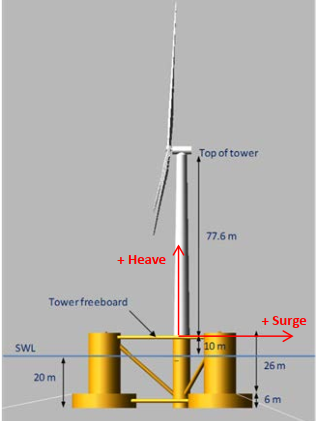
\includegraphics[width=0.99\textwidth]{OC4.png}
        \caption{\small OC4-DeepCwind floating wind system design. \cite{Robertson2014}}
        \label{fig:OC4}
    \end{minipage}
    \hfill
    \begin{minipage}{0.5\textwidth}
        \centering
        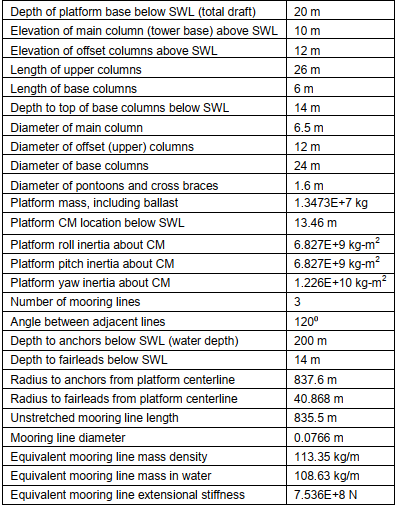
\includegraphics[width=0.97\textwidth]{characteristics.png}
        \caption{\small Summary of semisubmersible properties \cite{Robertson2014}}
        \label{fig:characteristics}
    \end{minipage}
\end{figure}

\begin{table}[H]
    \centering
    \caption{Load cases run in OC4 Phase II. \cite{Robertson2014}}
    \label{tab:image_table}
    \begin{tabular}{c}
        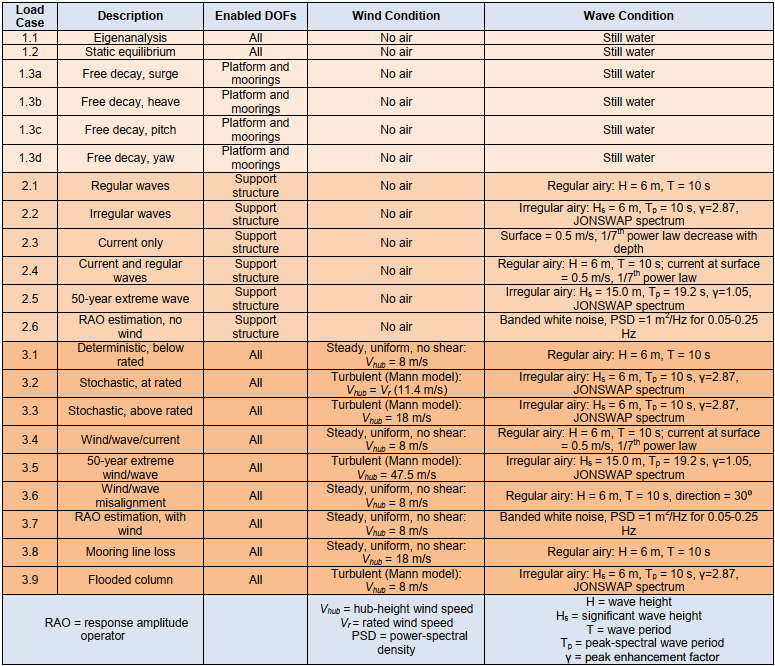
\includegraphics[width=1\textwidth]{table_3.png} \\
    \end{tabular}
\end{table}


\section{Pre-existing Model Analysis}

\hspace*{0.5cm}In this section, the analysis of the OC4 semisubmersible platform was conducted using a pre-existing model in OpenFAST called "marin\_semi". The model was subjected to free decay tests, as well as  wave and wind induced load cases, namely Group 1.3X, 2.X, and 3.X, as outlined in the study by Robertson et al. \cite{Robertson2014}. The results were processed using BEMRosetta to extract natural frequencies and generate response graphs.

\subsection{Free Decay Tests}
\hspace*{0.5cm}The free decay tests involves subjecting the platform to initial displacements and allowing it to oscillate freely. Each of the four cases from 1.3a to 1.3d analyze the four individual degrees of freedom, specifically surge, heave, pitch, and yaw. The platform is given an initial displacement in the respective degree of freedom for each load case. The motion response of the platform was calculated using OpenFAST, and the natural frequencies were extracted from the time-domain data using the Fast Fourier Transform (FFT) method on BEMRosetta. The motion results of the 1.3a and 1.3b can be seen in Figures~\ref{fig:1.3a_surge}--\ref{fig:1.3b_pitch_mine}. The natural frequencies obtained from the tests for 6 degrees of freedom are shown in Figures ~\ref{fig:nat_freq_surge}--\ref{fig:nat_freq_yaw} and consistent with the reference study, confirming the accuracy of the modeling approach (\autoref{fig:nat_freq}).
\vspace{0.3cm}

%%1.3a figures
\begin{figure}[H]
    \begin{minipage}{0.48\textwidth}
        \centering
        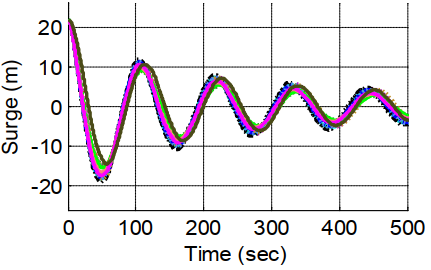
\includegraphics[width=0.97\textwidth]{1.3a_surge.png}
        \caption{\small Surge free decay platform motion response for load case 1.3a \cite{Robertson2014}}
        \label{fig:1.3a_surge}
    \end{minipage}
    \hfill
    \begin{minipage}{0.49\textwidth}
        \centering
        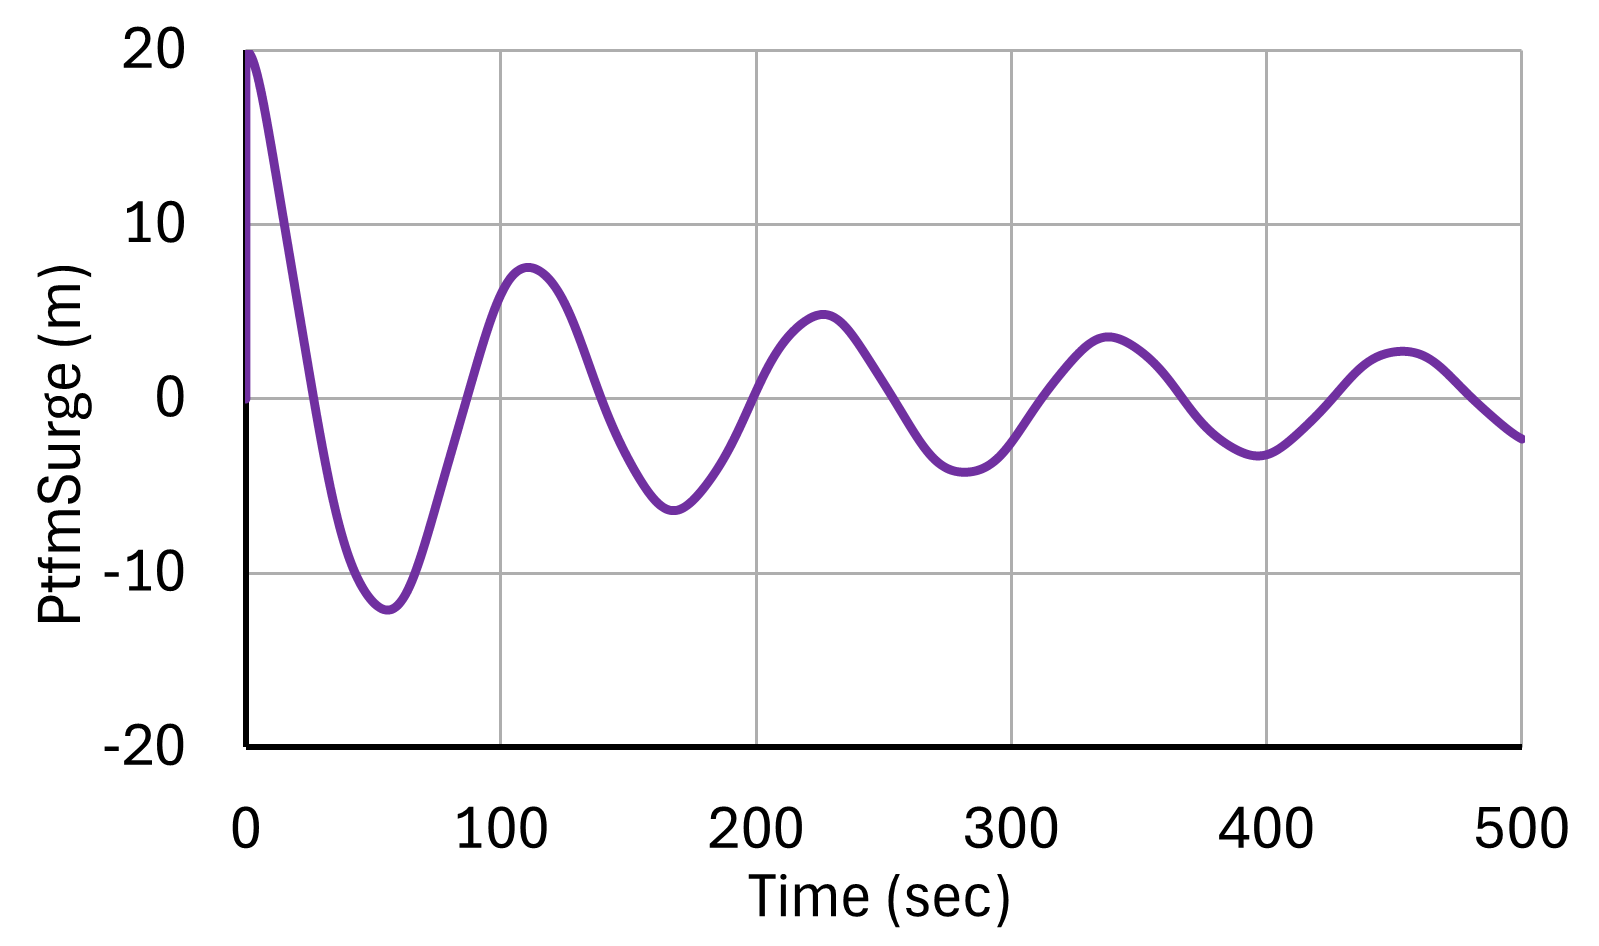
\includegraphics[width=1\textwidth]{1.3a_surge_mine.png}
        \caption{\small Surge free decay platform motion response for load case 1.3a}
        \label{fig:1.3a_surge_mine}
    \end{minipage}
\end{figure}

\begin{figure}[H]
    \begin{minipage}{0.48\textwidth}
        \centering
        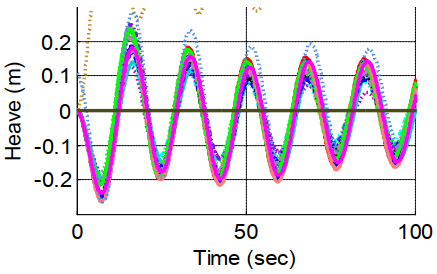
\includegraphics[width=0.97\textwidth]{1.3a_heave.png}
        \caption{\small Heave free decay platform motion response for load case 1.3a \cite{Robertson2014}}
        \label{fig:1.3a_heave}
    \end{minipage}
    \hfill
    \begin{minipage}{0.49\textwidth}
        \centering
        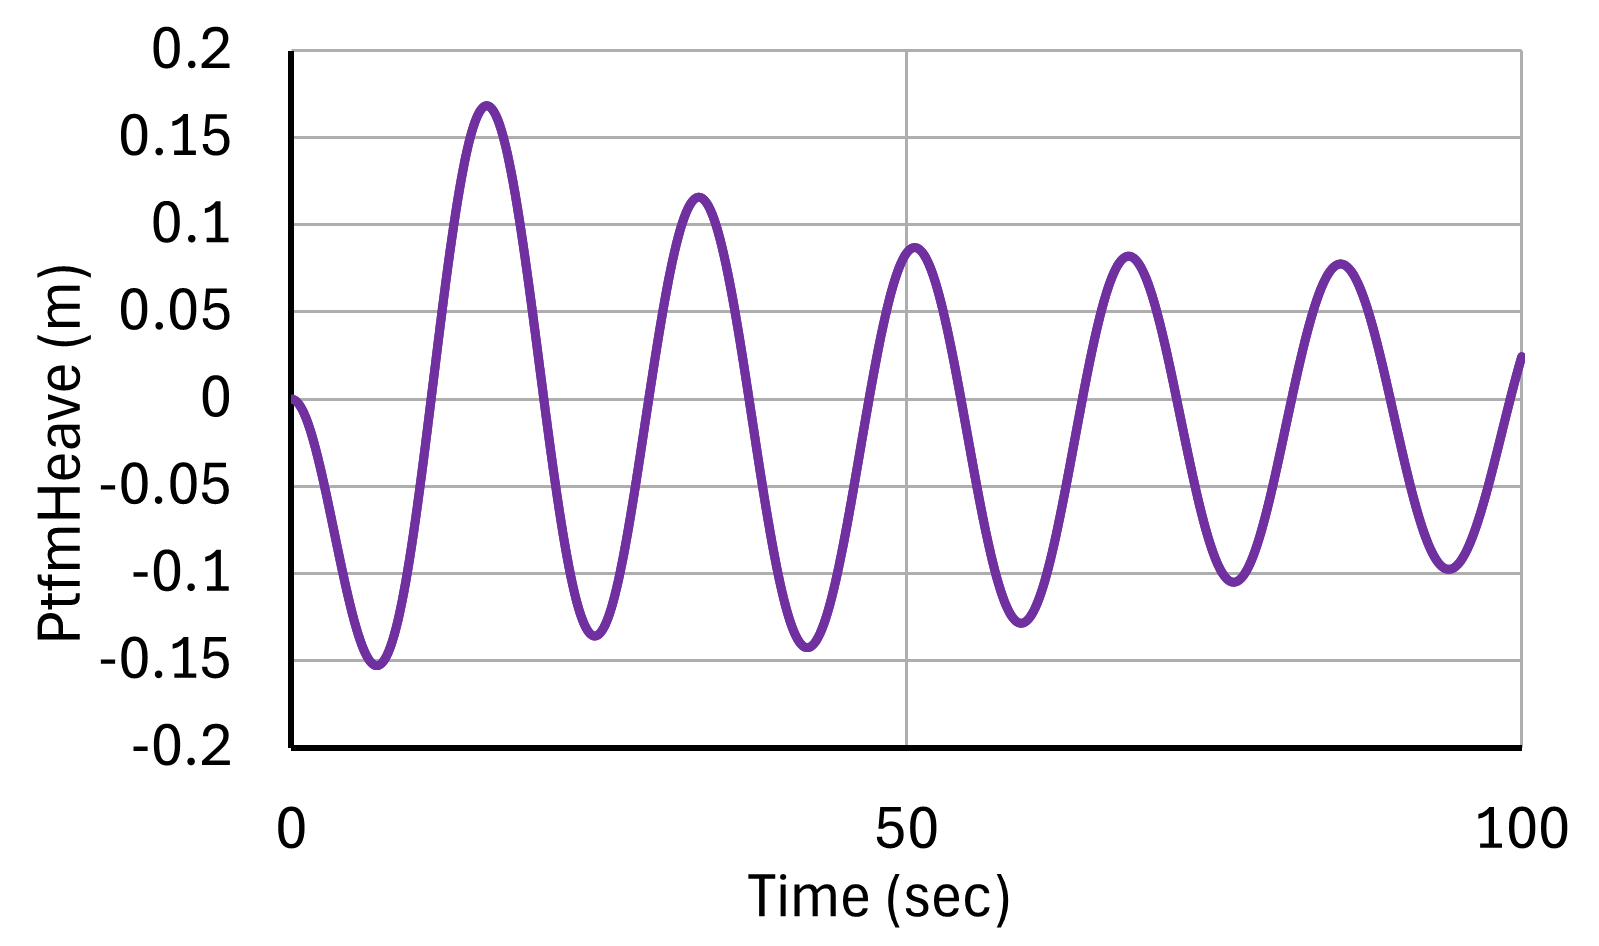
\includegraphics[width=1\textwidth]{1.3a_heave_mine.png}
        \caption{\small Heave free decay platform motion response for load case 1.3a}
        \label{fig:1.3a_heave_mine}
    \end{minipage}
\end{figure}

\begin{figure}[H]
    \begin{minipage}{0.48\textwidth}
        \centering
        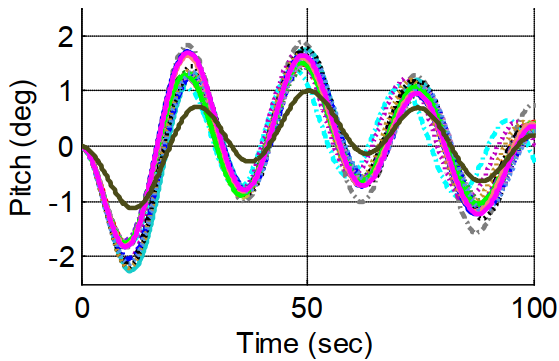
\includegraphics[width=0.97\textwidth]{1.3a_pitch.png}
        \caption{\small Pitch free decay platform motion response for load case 1.3a \cite{Robertson2014}}
        \label{fig:1.3a_pitch}
    \end{minipage}
    \hfill
    \begin{minipage}{0.49\textwidth}
        \centering
        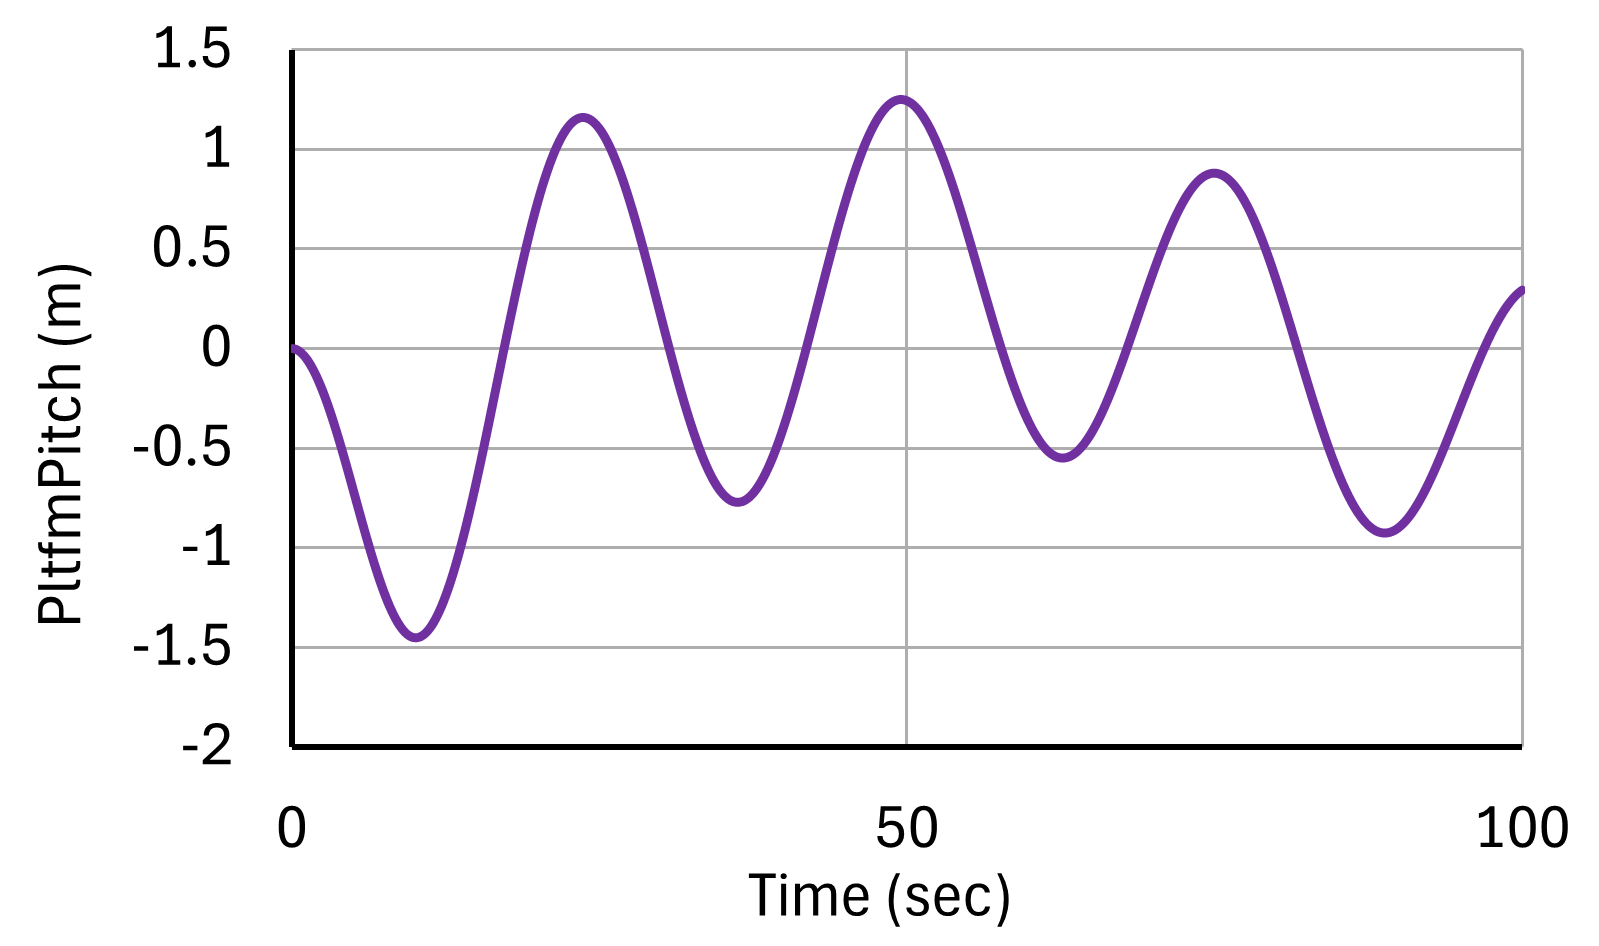
\includegraphics[width=1\textwidth]{1.3a_pitch_mine.png}
        \caption{\small Pitch free decay platform motion response for load case 1.3a}
        \label{fig:1.3a_pitch_mine}
    \end{minipage}
\end{figure}

%%1.3b figures
\begin{figure}[H]
    \begin{minipage}{0.47\textwidth}
        \centering
        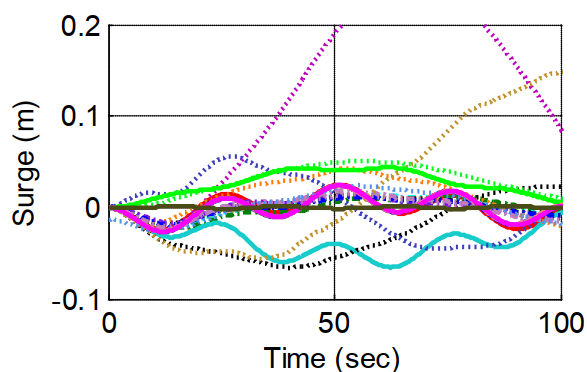
\includegraphics[width=0.97\textwidth]{1.3b_surge.png}
        \caption{\small Surge free decay platform motion response for load case 1.3b \cite{Robertson2014}}
        \label{fig:1.3b_surge}
    \end{minipage}
    \hfill
    \begin{minipage}{0.5\textwidth}
        \centering
        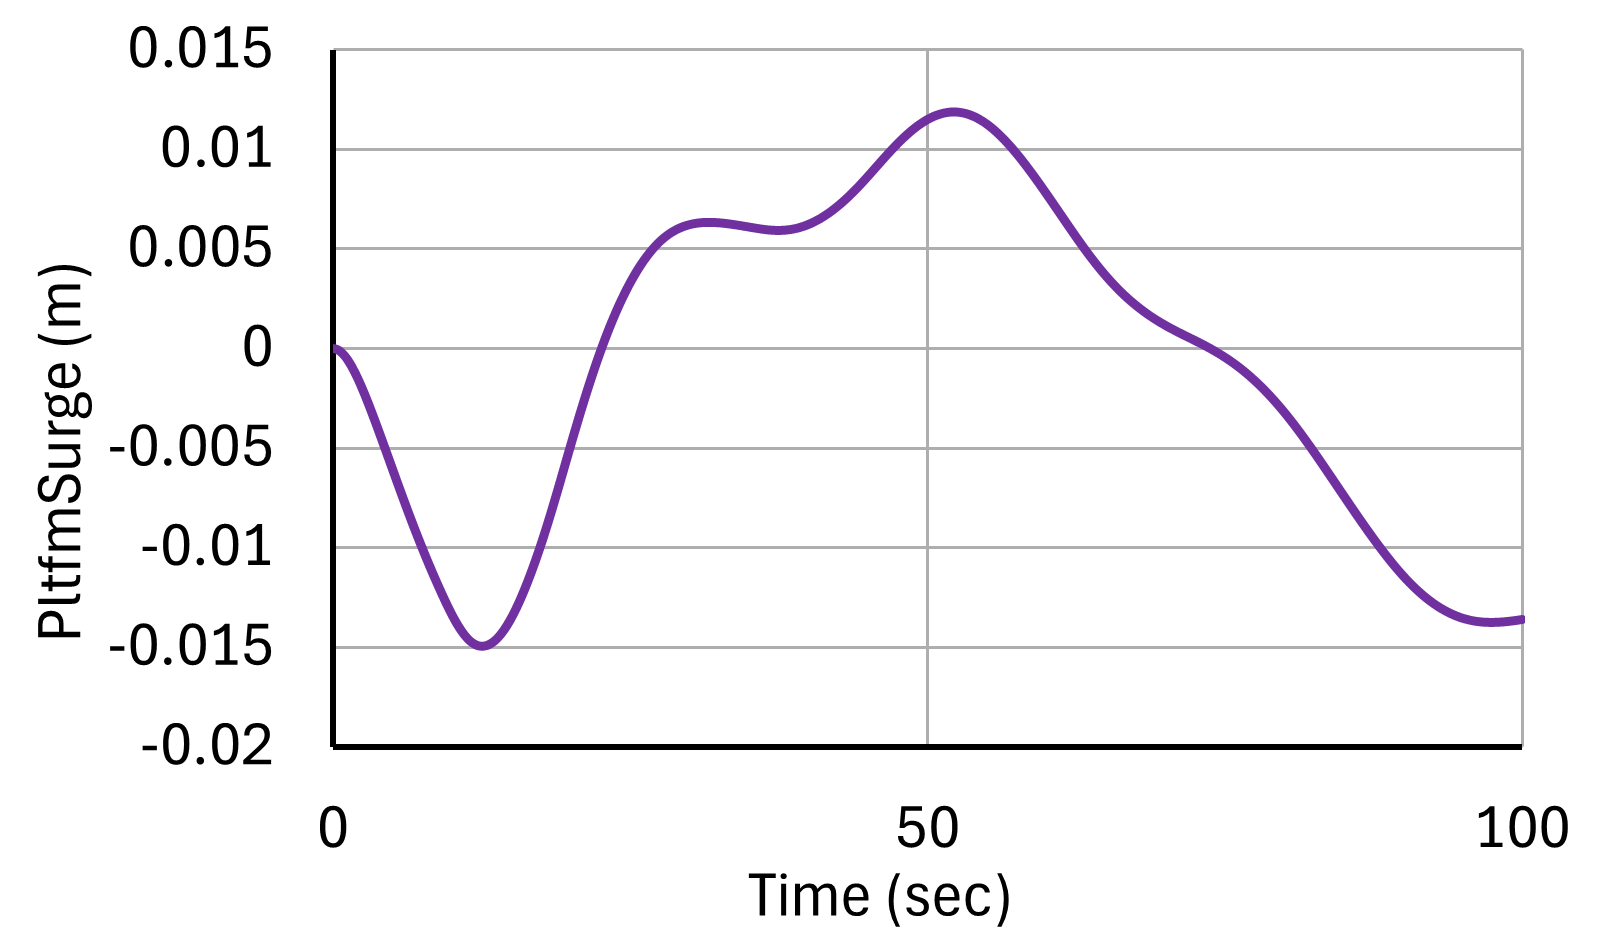
\includegraphics[width=1\textwidth]{1.3b_surge_mine.png}
        \caption{\small Surge free decay platform motion response for load case 1.3b}
        \label{fig:1.3b_surge_mine}
    \end{minipage}
\end{figure}

\begin{figure}[H]
    \begin{minipage}{0.47\textwidth}
        \centering
        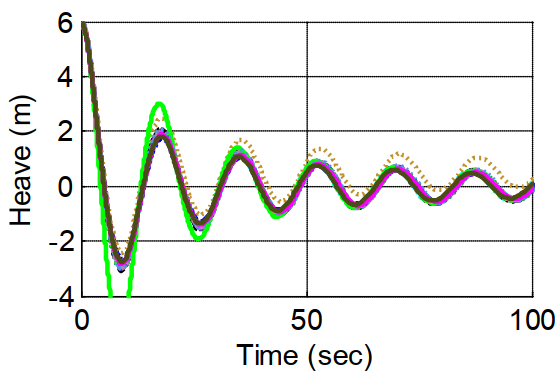
\includegraphics[width=0.97\textwidth]{1.3b_heave.png}
        \caption{\small Heave free decay platform motion response for load case 1.3b \cite{Robertson2014}}
        \label{fig:1.3b_heave}
    \end{minipage}
    \hfill
    \begin{minipage}{0.5\textwidth}
        \centering
        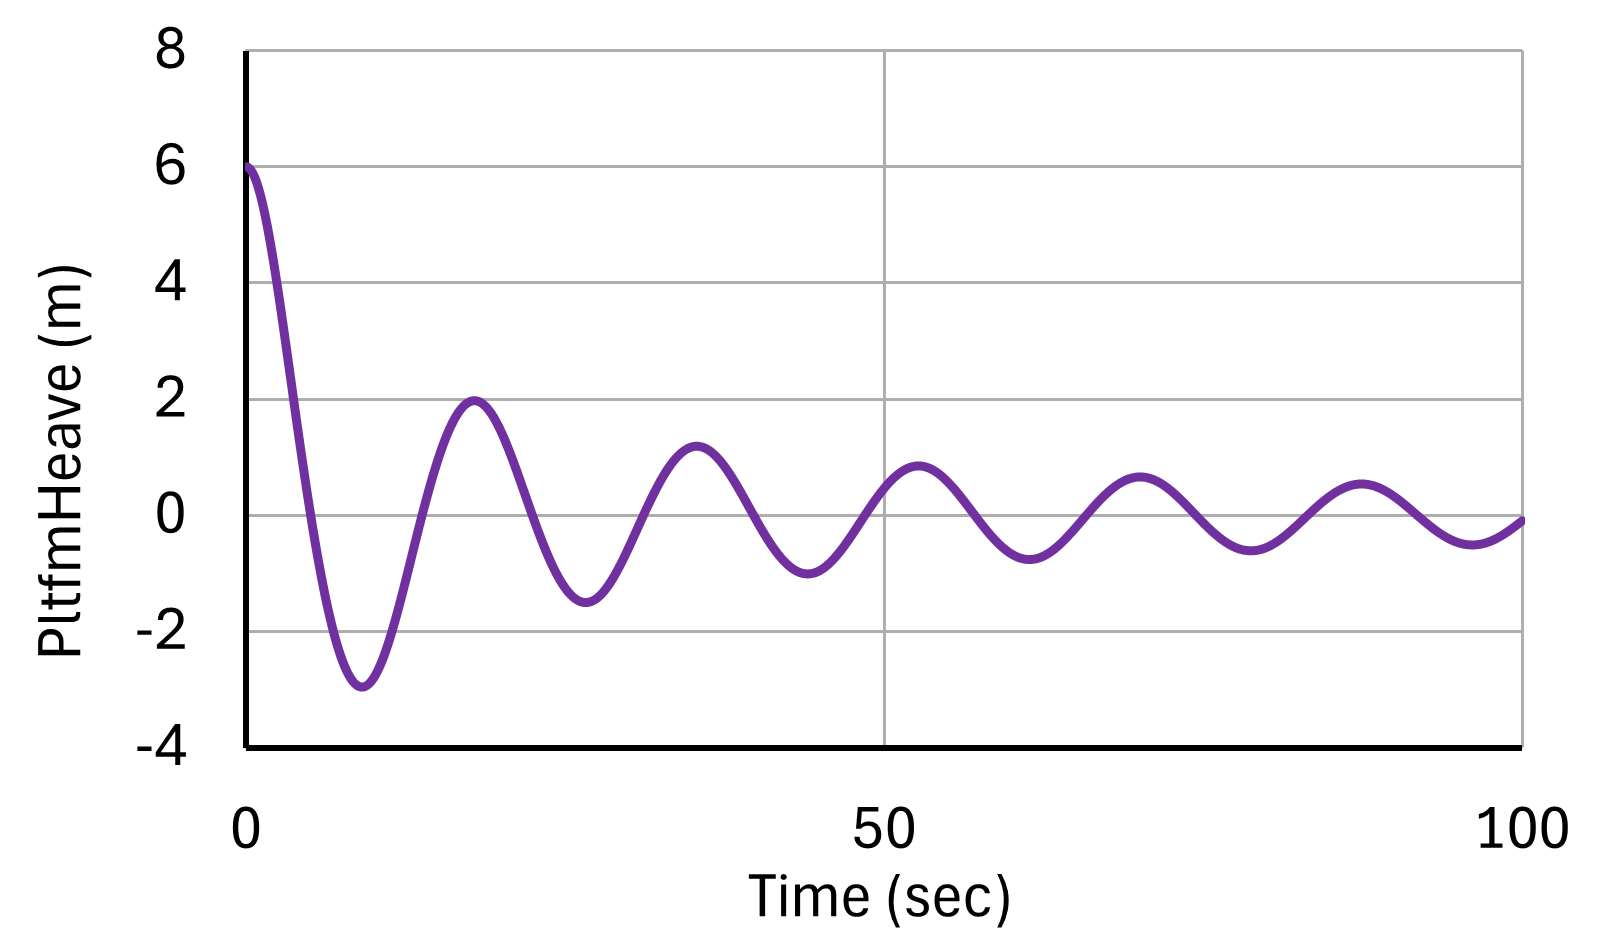
\includegraphics[width=1\textwidth]{1.3b_heave_mine.png}
        \caption{\small Heave free decay platform motion response for load case 1.3b}
        \label{fig:1.3b_heave_mine}
    \end{minipage}
\end{figure}

\begin{figure}[H]
    \begin{minipage}{0.47\textwidth}
        \centering
        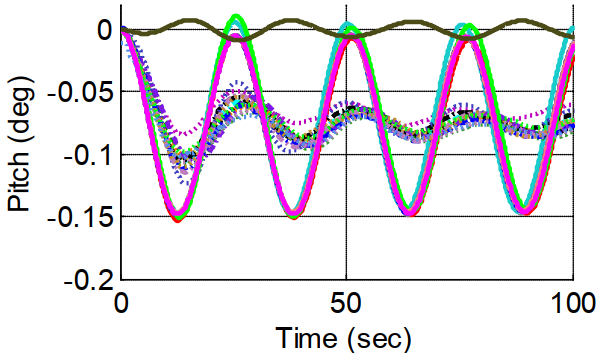
\includegraphics[width=0.97\textwidth]{1.3b_pitch.png}
        \caption{\small Pitch free decay platform motion response for load case 1.3b \cite{Robertson2014}}
        \label{fig:1.3b_pitch}
    \end{minipage}
    \hfill
    \begin{minipage}{0.5\textwidth}
        \centering
        \vspace{-0.3cm}
        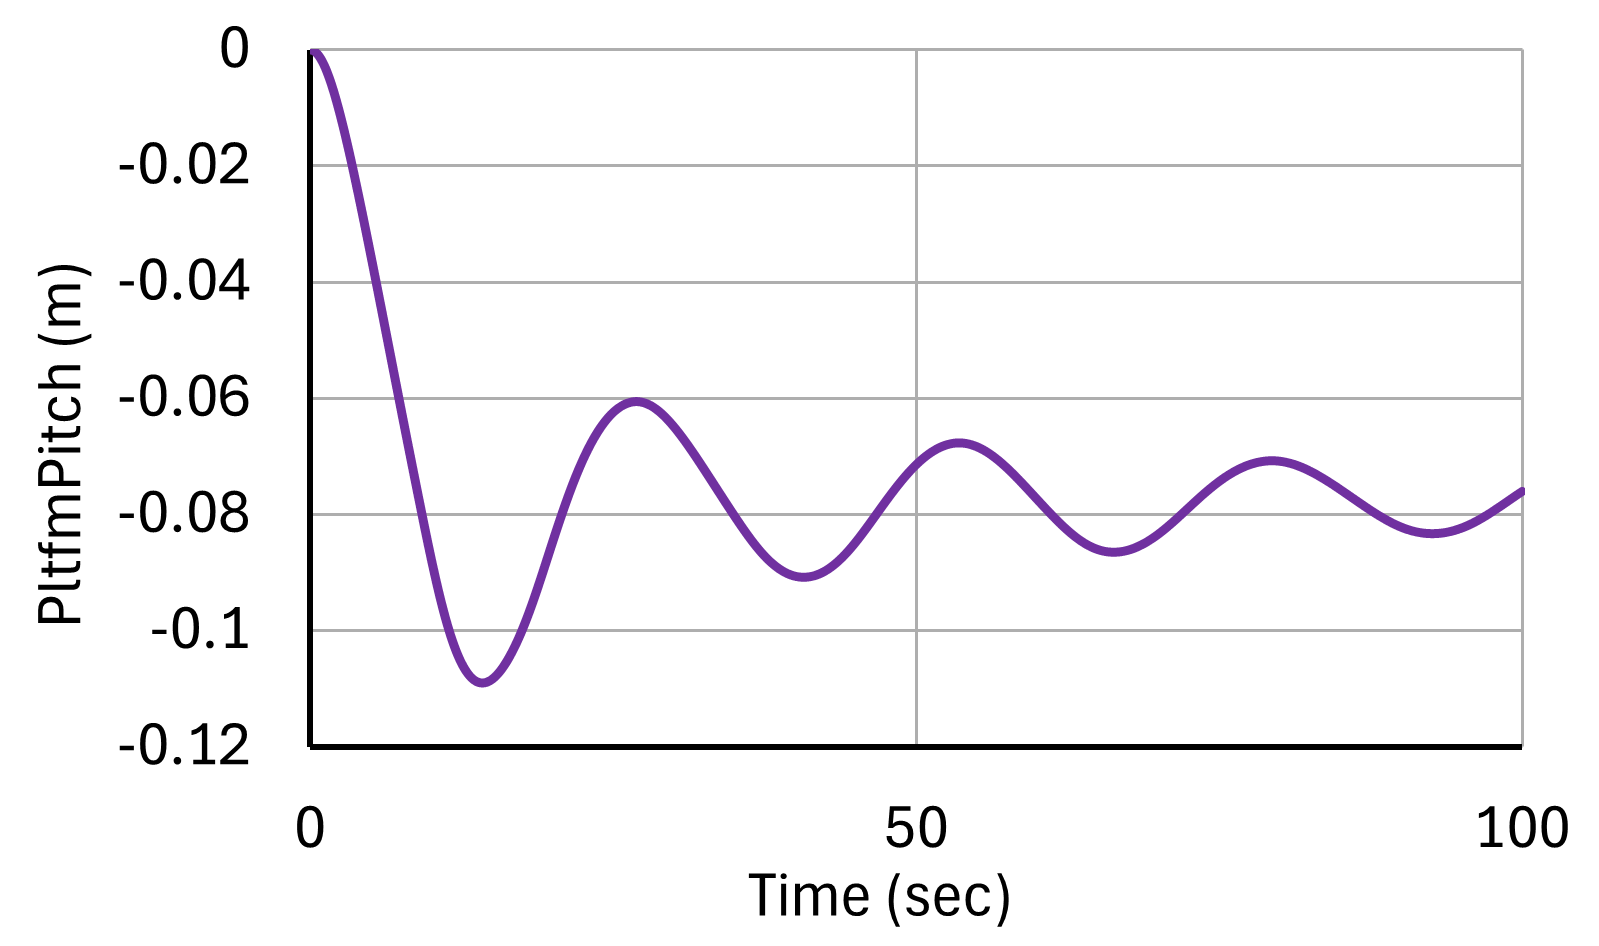
\includegraphics[width=1\textwidth]{1.3b_pitch_mine.png}
        \caption{\small Pitch free decay platform motion response for load case 1.3b}
        \label{fig:1.3b_pitch_mine}
    \end{minipage}
\end{figure}

When the graphs plotted for the surge, heave, and pitch motions are compared to the reference study, it can be observed that the results are consistent in terms of the overall pattern of the motion response. Specifically, for the 1.3b case, the pitch motion response shows a very close resemblance to the distinct grouping using Morison’s equation for calculating the viscous drag (dotted or dash-dotted results) versus those using a quadratic drag matrix (solid line results).

%%natural frequencies

\begin{figure}[H]
    \centering
    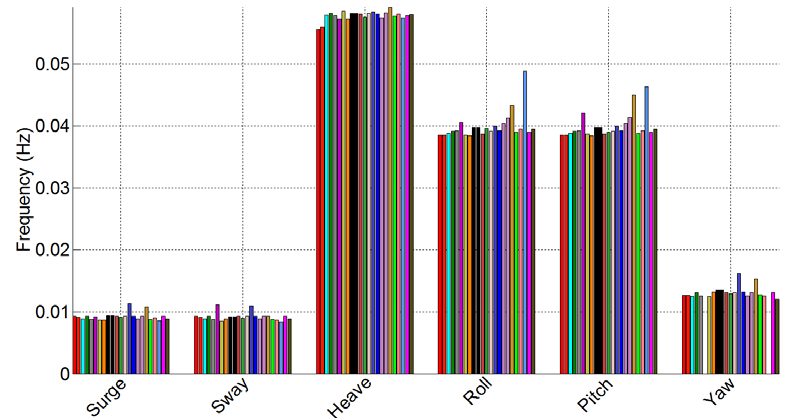
\includegraphics[width=0.9\textwidth]{nat_freq.png}
    \caption{\small Full-system natural frequencies \cite{Robertson2014}}
    \label{fig:nat_freq}
\end{figure}

\begin{figure}[H]
    \begin{minipage}{0.49\textwidth}
        \centering
        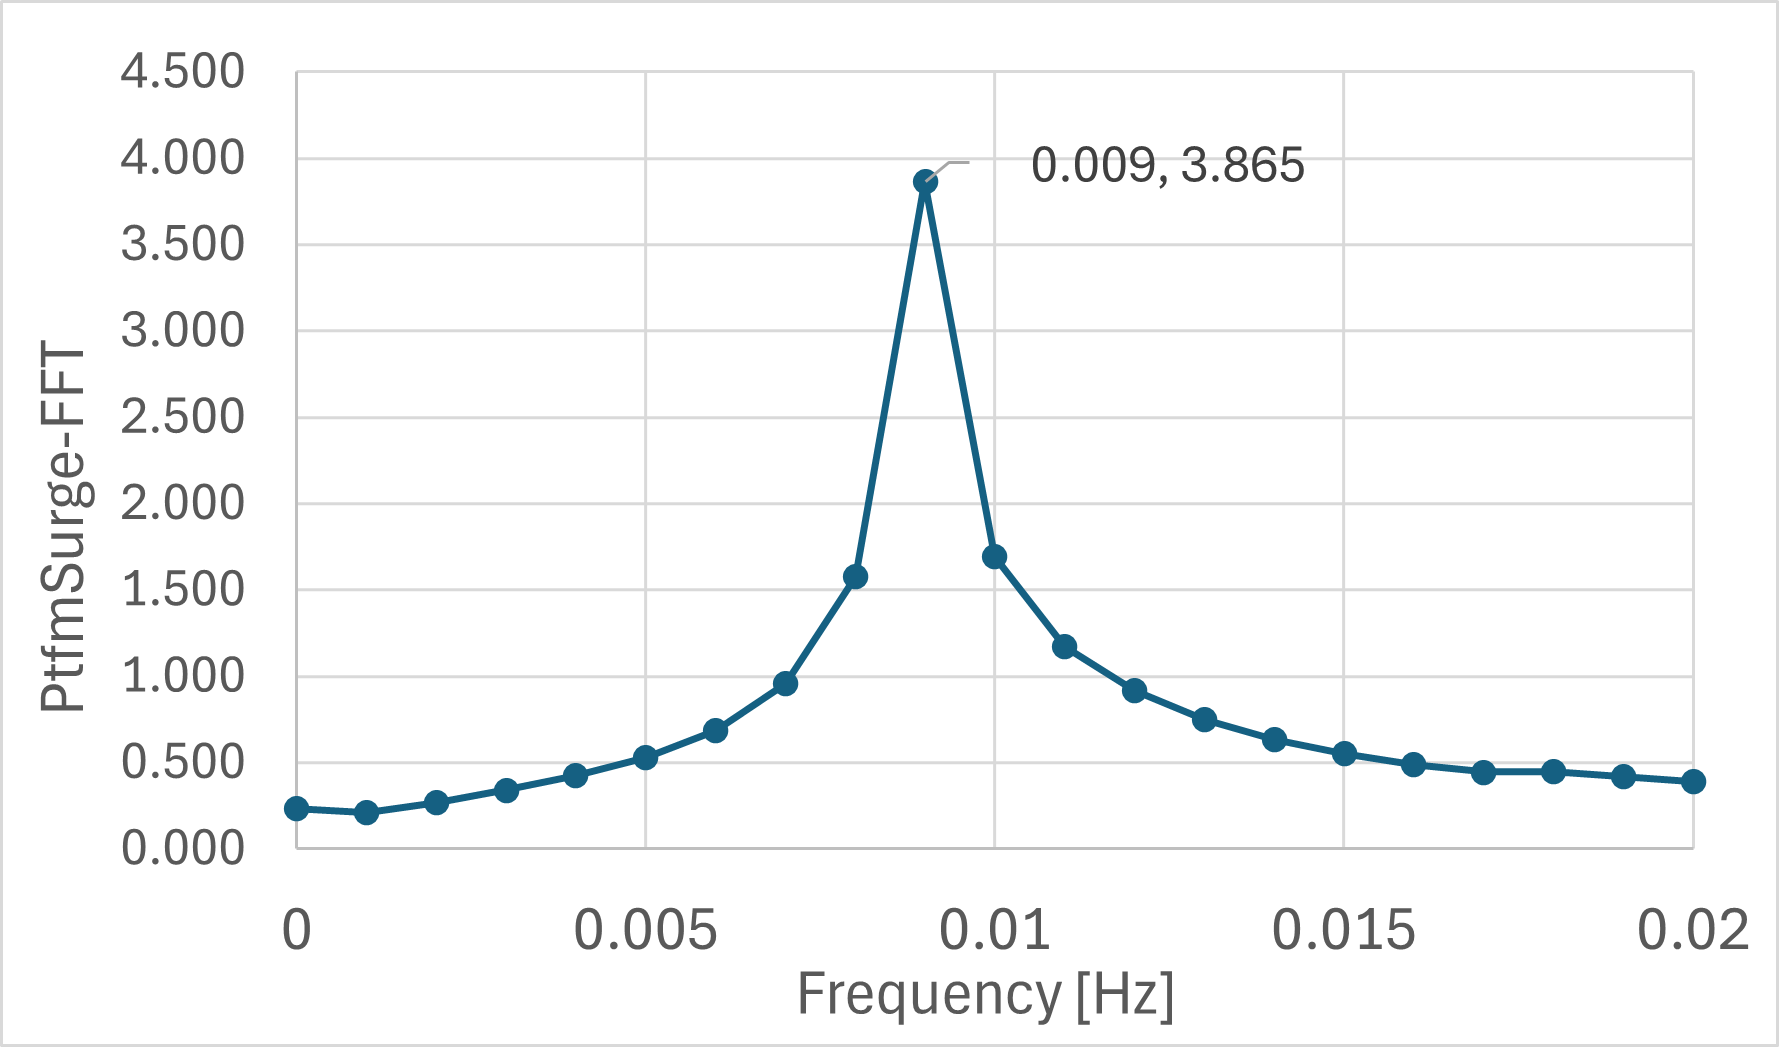
\includegraphics[width=1\textwidth]{nat_freq_surge.png}
        \caption{\small Surge natural frequency}
        \label{fig:nat_freq_surge}
    \end{minipage}
    \hfill
    \begin{minipage}{0.5\textwidth}
        \centering
        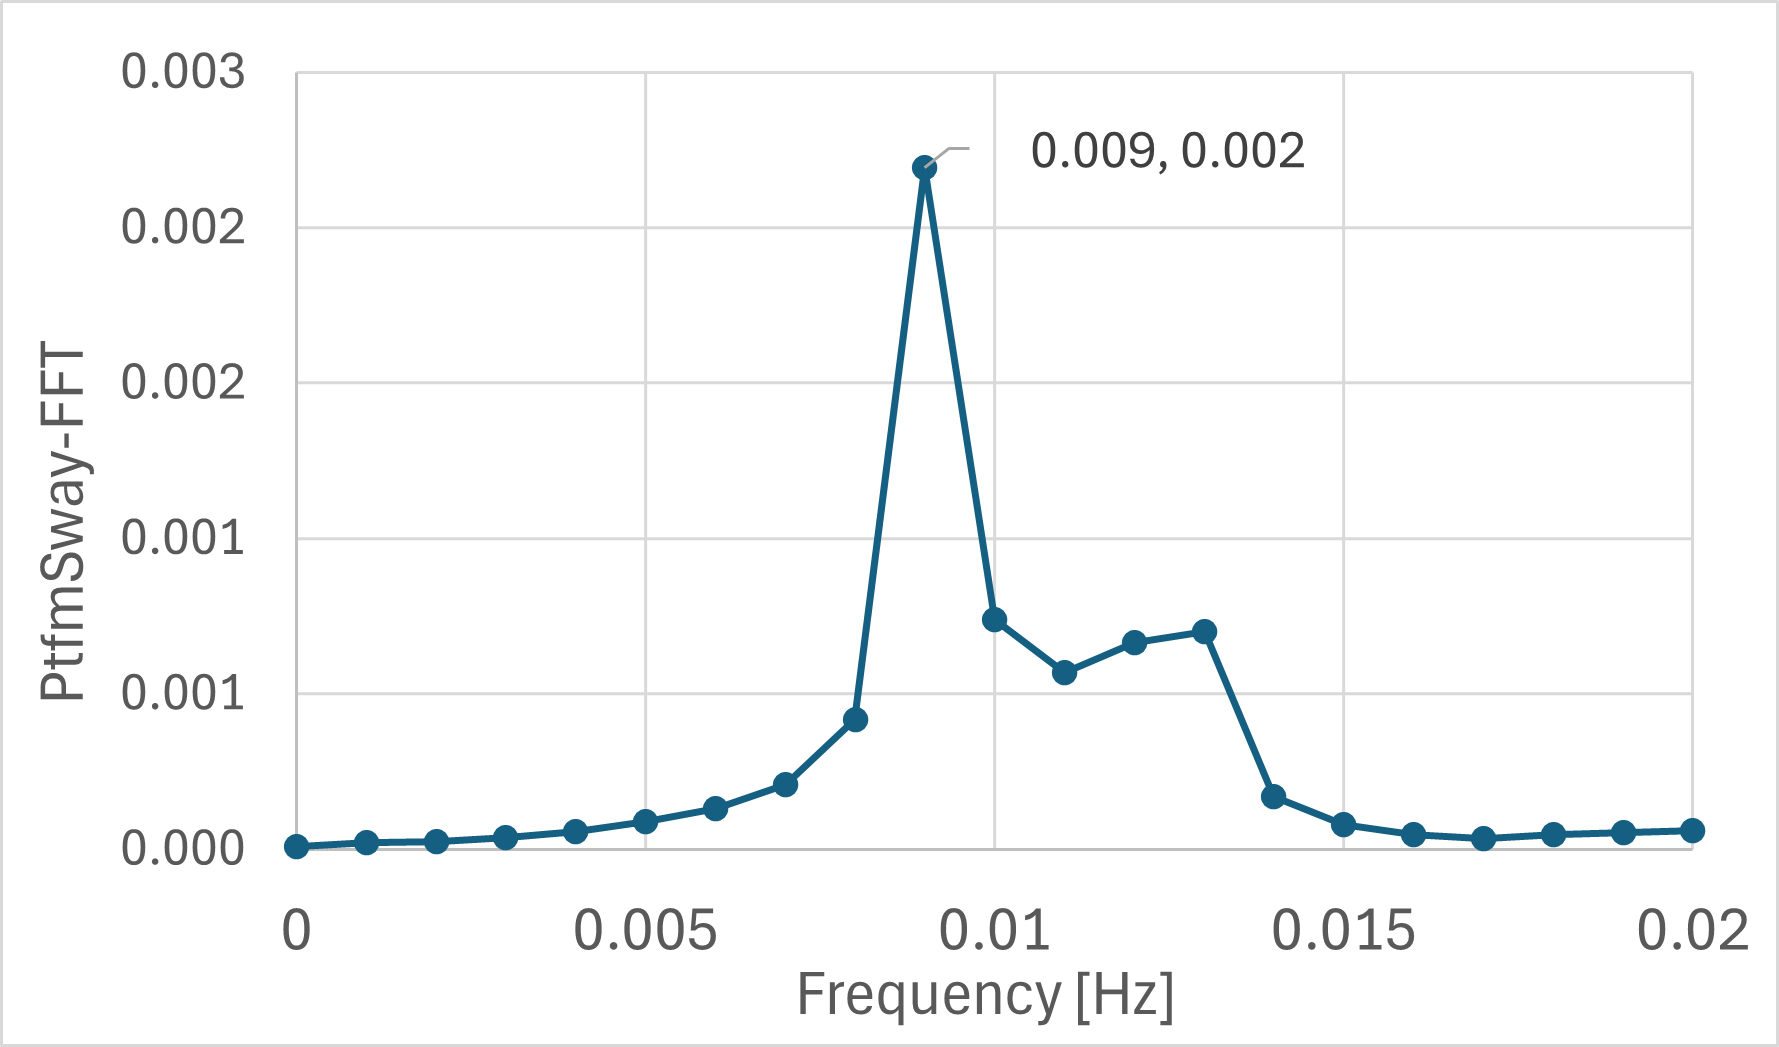
\includegraphics[width=1\textwidth]{nat_freq_sway.png}
        \caption{\small Sway natural frequency}
        \label{fig:nat_freq_sway}
    \end{minipage}
\end{figure}

\begin{figure}[H]
    \begin{minipage}{0.49\textwidth}
        \centering
        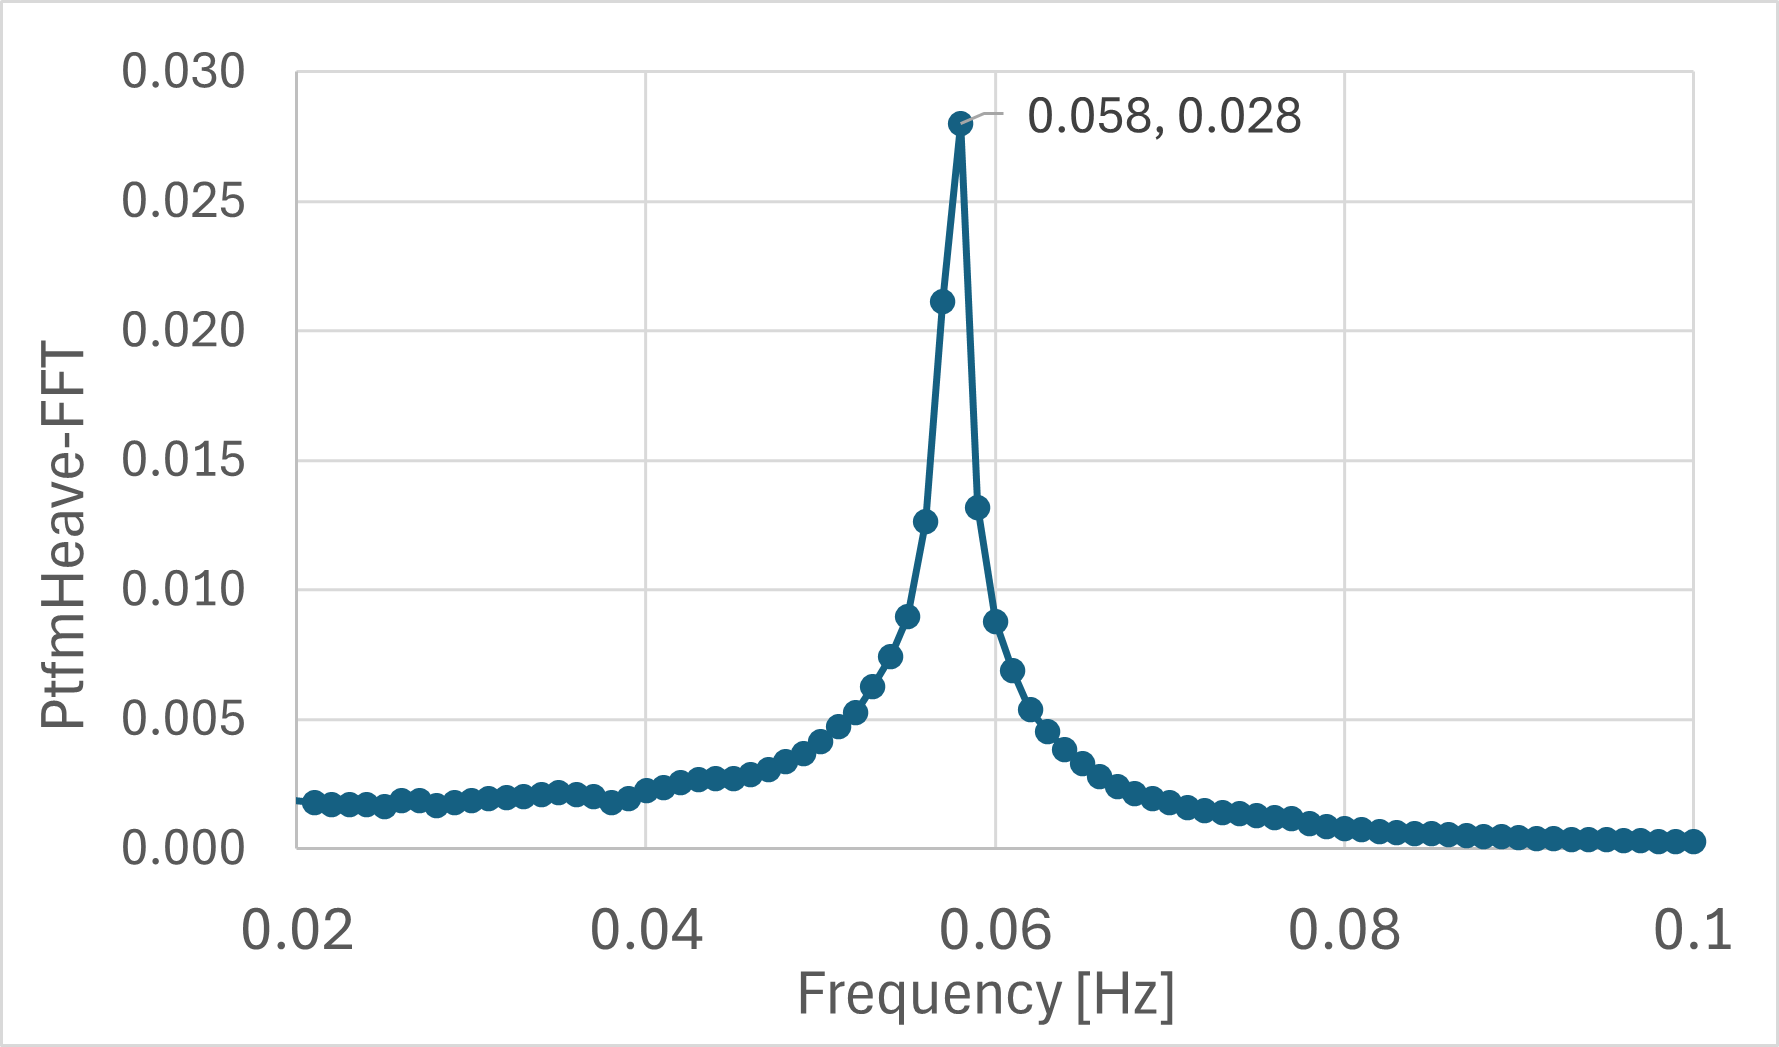
\includegraphics[width=1\textwidth]{nat_freq_heave.png}
        \caption{\small Heave natural frequency}
        \label{fig:nat_freq_heave}
    \end{minipage}
    \hfill
    \begin{minipage}{0.5\textwidth}
        \centering
        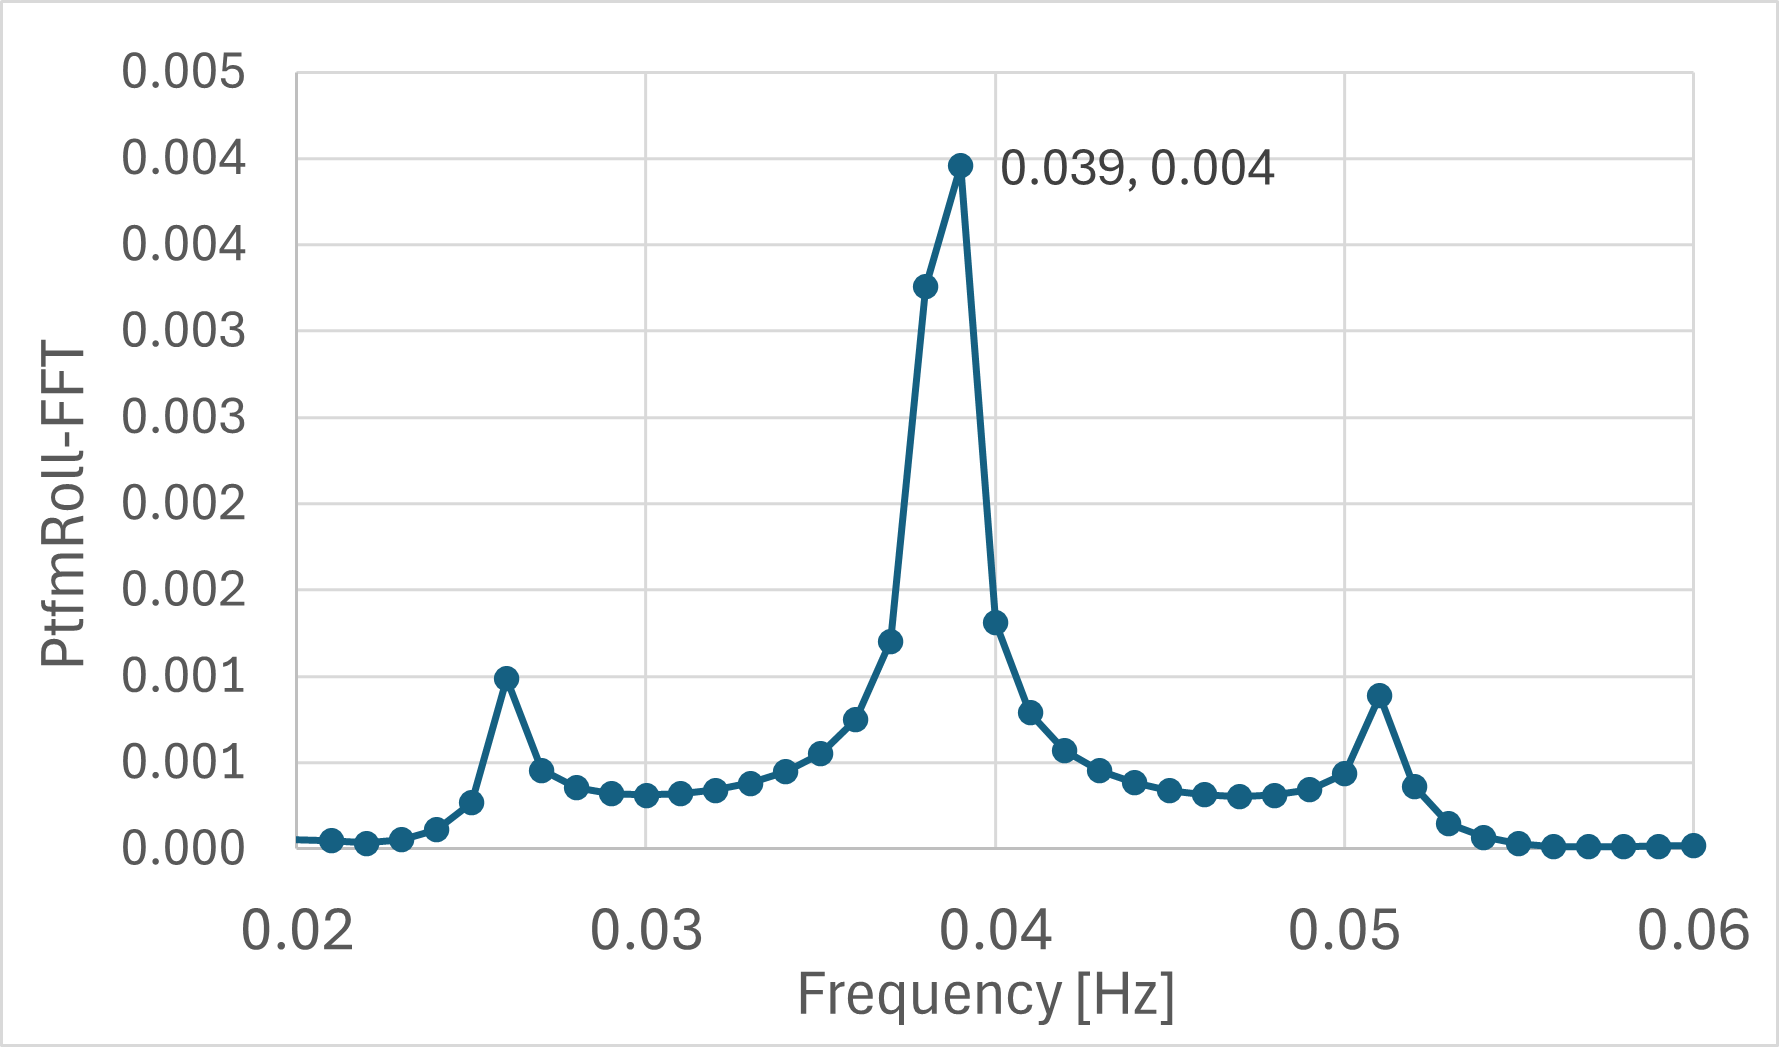
\includegraphics[width=1\textwidth]{nat_freq_roll.png}
        \caption{\small Roll natural frequency}
        \label{fig:nat_freq_roll}
    \end{minipage}
\end{figure}

\begin{figure}[H]
    \begin{minipage}{0.49\textwidth}
        \centering
        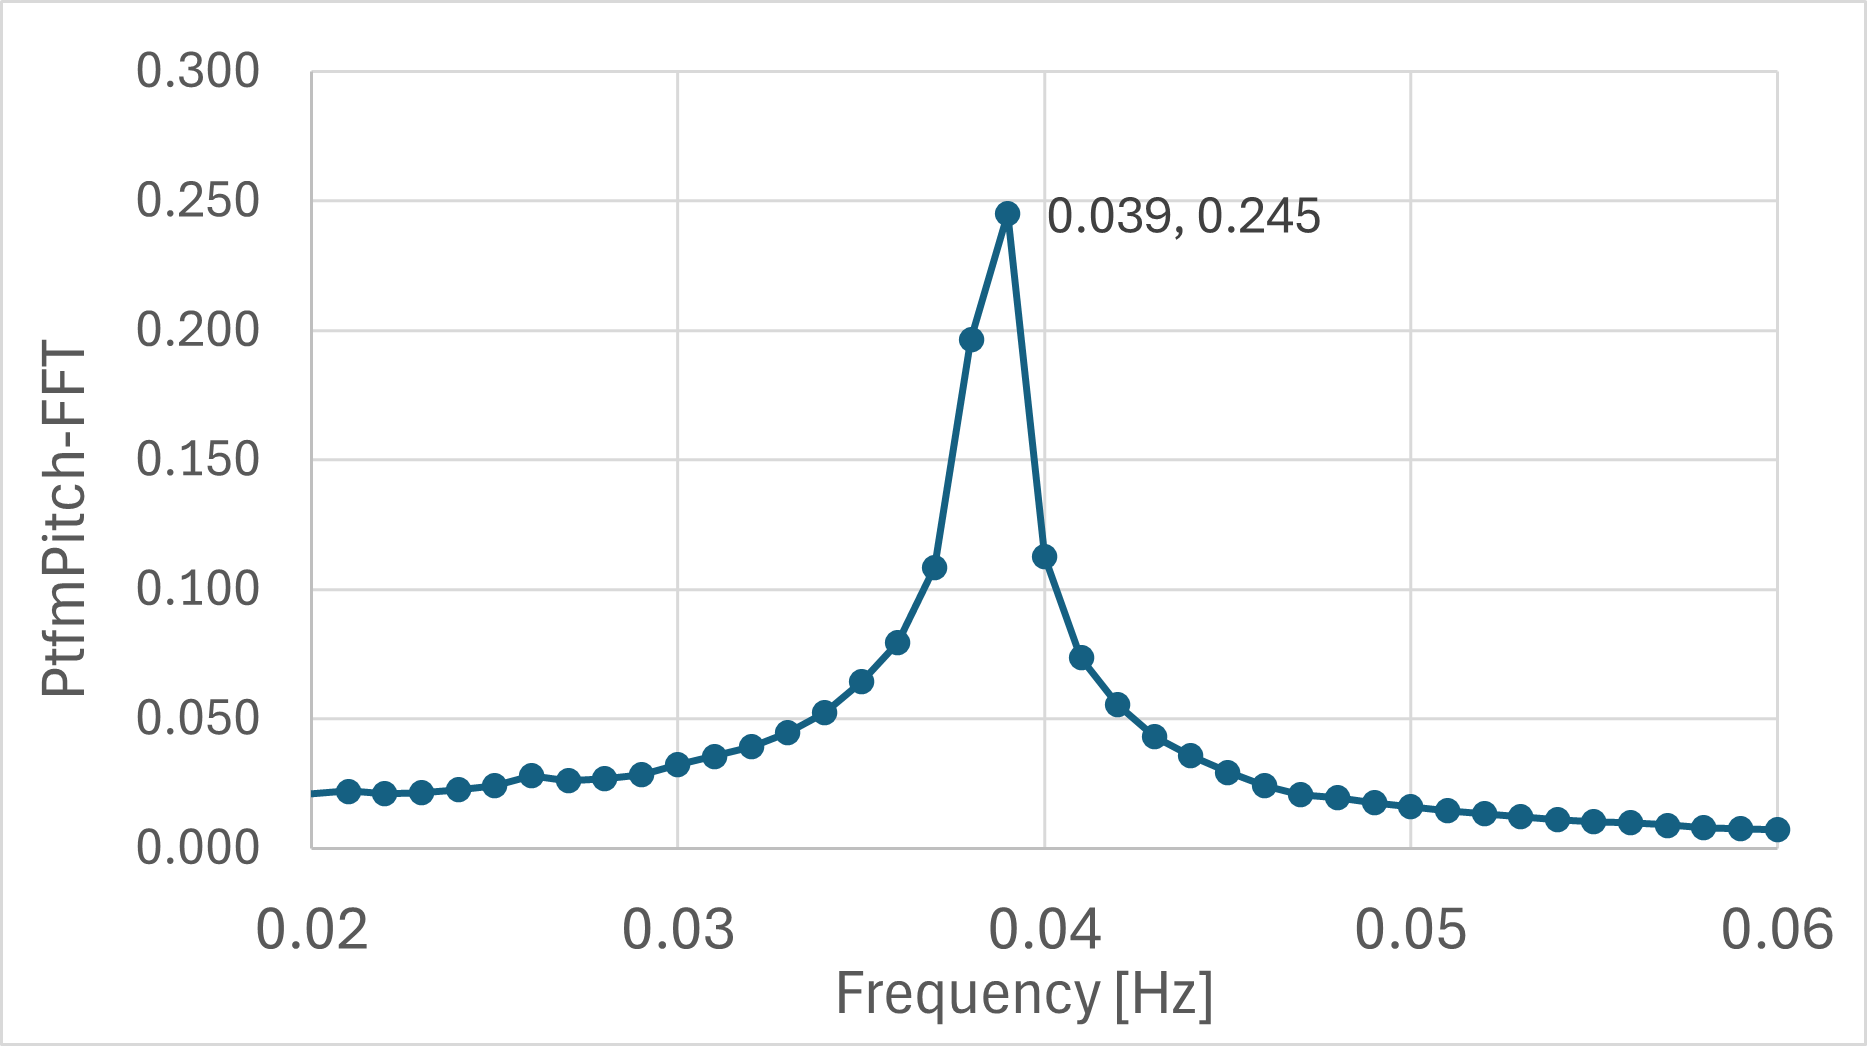
\includegraphics[width=1\textwidth]{nat_freq_pitch.png}
        \caption{\small Pitch natural frequency}
        \label{fig:nat_freq_pitch}
    \end{minipage}
    \hfill
    \begin{minipage}{0.5\textwidth}
        \centering
        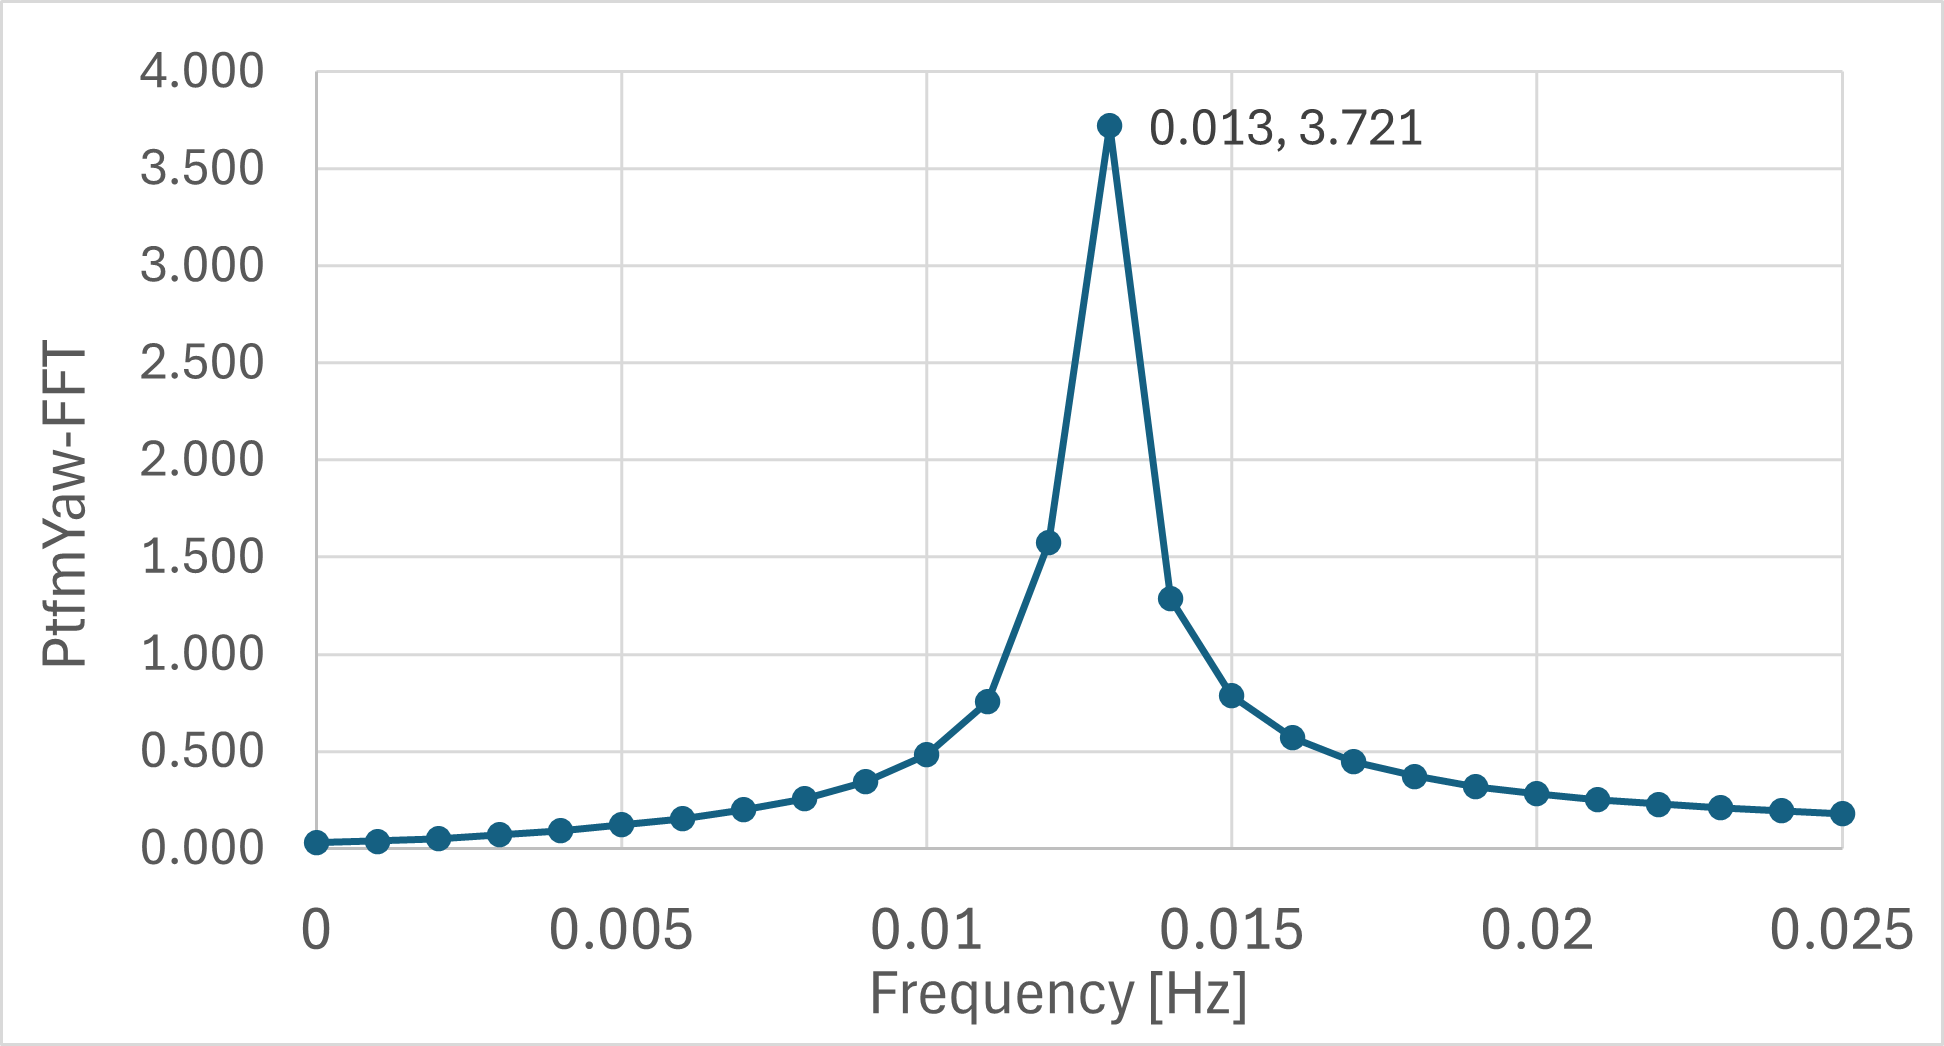
\includegraphics[width=1\textwidth]{nat_freq_yaw.png}
        \caption{\small Yaw natural frequency}
        \label{fig:nat_freq_yaw}
    \end{minipage}
\end{figure}

The natural frequency analysis of the semisubmersible platform shows clear differences in the magnitude of these frequencies across the six degrees of freedom. Specifically, the natural frequencies for heave, roll and pitch were notably higher than those for surge, sway and yaw, with heave demonstrating highest frequency overall.

This difference originates from the restoring mechanisms associated with each degree of freedom. Heave, roll, and pitch are governed by strong hydrostatic restoring forces. For heave, this is primarily due to buoyancy, where vertical displacements lead to significant changes in the buoyant force. Roll and pitch experience restoring moments due to the platform's metacentric heights, which resist angular displacements. These restoring forces result in higher natural frequencies. In contrast, the restoring forces for surge and sway are minimal for small displacements, leading to very low natural frequencies. The yaw response shows restoring strength of similar but reduced magnitude to roll and pitch. This rotational stiffness is primarily from hydrodynamic sources like the geometry of the body, rather than the hydrostatic mechanisms that dominate roll and pitch \cite{metacenter}.


\subsection{Wave and Current Induced Tests}
\hspace*{0.5cm}The wave and current induced tests were conducted to analyze the platform's response to various environmental conditions, including regular and irregular waves, as well as current effects. The load cases were selected from the reference study by Robertson et al. \cite{Robertson2014} and included Group 2.X load cases. The results were processed using BEMRosetta to extract the platform's motion responses and mooring tensions.

\subsubsection{Load Case 2.1}

\hspace{0.5cm}Load case 2.1 was used to analyze the platform’s response to regular waves, focusing on heave, pitch, surge motions, and the tension force at fairlead 2. The analysis was conducted using two approaches: one incorporating second-order drift effects through quadratic transfer functions (QTF) to account for low-frequency wave forces, and another excluding drift effects to isolate first-order wave responses. The results, processed using BEMRosetta, were compared to the reference study (Figures~\ref{fig:2.1_surge}--\ref{fig:2.1_fairten2_mine}).

The platform's motion responses showed a strong resemblence to NREL's FAST v8 simulations when drift effects were neglected, as expected, since they did not utilize QTF-based second-order analysis in their calculations. This alignment confirms that both approaches produced equivalent first-order hydrodynamic responses. This consistency validates the first-order hydrodynamic modeling approach. However, when drift forces were introduced, surge motion showed significant sensitivity to QTF inclusion due to its weak hydrodynamic restoring forces. In contrast, heave and pitch motions remained relatively unaffected by second-order effects because of their strong hydrostatic stiffness and higher natural frequencies (Figures~\ref{fig:nat_freq_heave} and~\ref{fig:nat_freq_pitch}) making them more responsive to first-order wave excitations. The reduction in maximum fairlead 2 tension when neglecting QTF stems from this mooring point's  coupling with surge motion along the y-axis. These tension results aligned with dynamic mooring models, validating that the simulation properly accounted for the mooring system's mass, stiffness, and damping characteristics.

%% 2.1 figures
\begin{figure}[H]
    \begin{minipage}{0.48\textwidth}
        \centering
        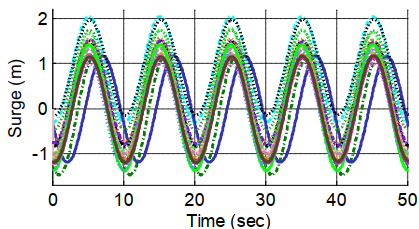
\includegraphics[width=1\textwidth]{2.1_surge.png}
        \caption{\small Surge response \cite{Robertson2014}}
        \label{fig:2.1_surge}
    \end{minipage}
    \hfill
    \begin{minipage}{0.51\textwidth}
        \centering
        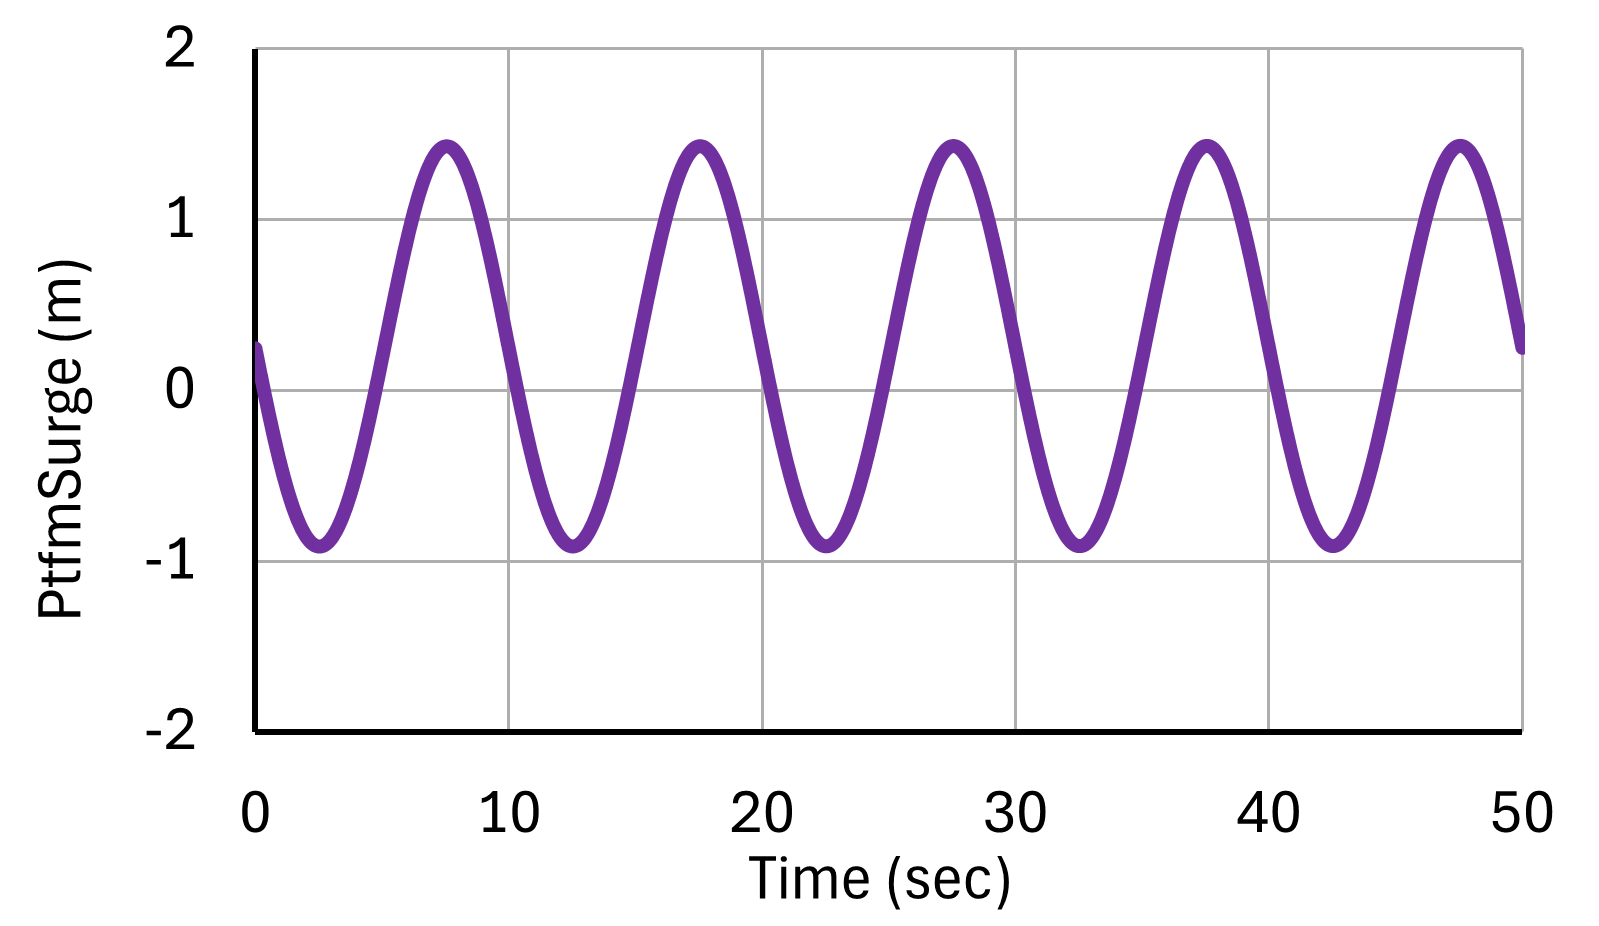
\includegraphics[width=1\textwidth]{2.1_surge_mine.png}
        \caption{\small Surge response}
        \label{fig:2.1_surge_mine}
    \end{minipage}
\end{figure}
\vspace{-0.2cm}
\begin{figure}[H]
    \begin{minipage}{0.48\textwidth}
        \centering
        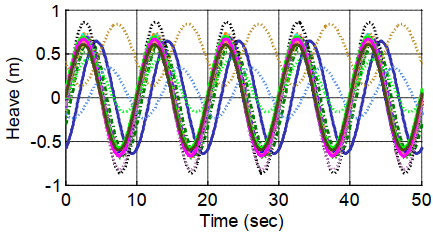
\includegraphics[width=1\textwidth]{2.1_heave.png}
        \caption{\small Heave response \cite{Robertson2014}}
        \label{fig:2.1_heave}
    \end{minipage}
    \hfill
    \begin{minipage}{0.51\textwidth}
        \centering
        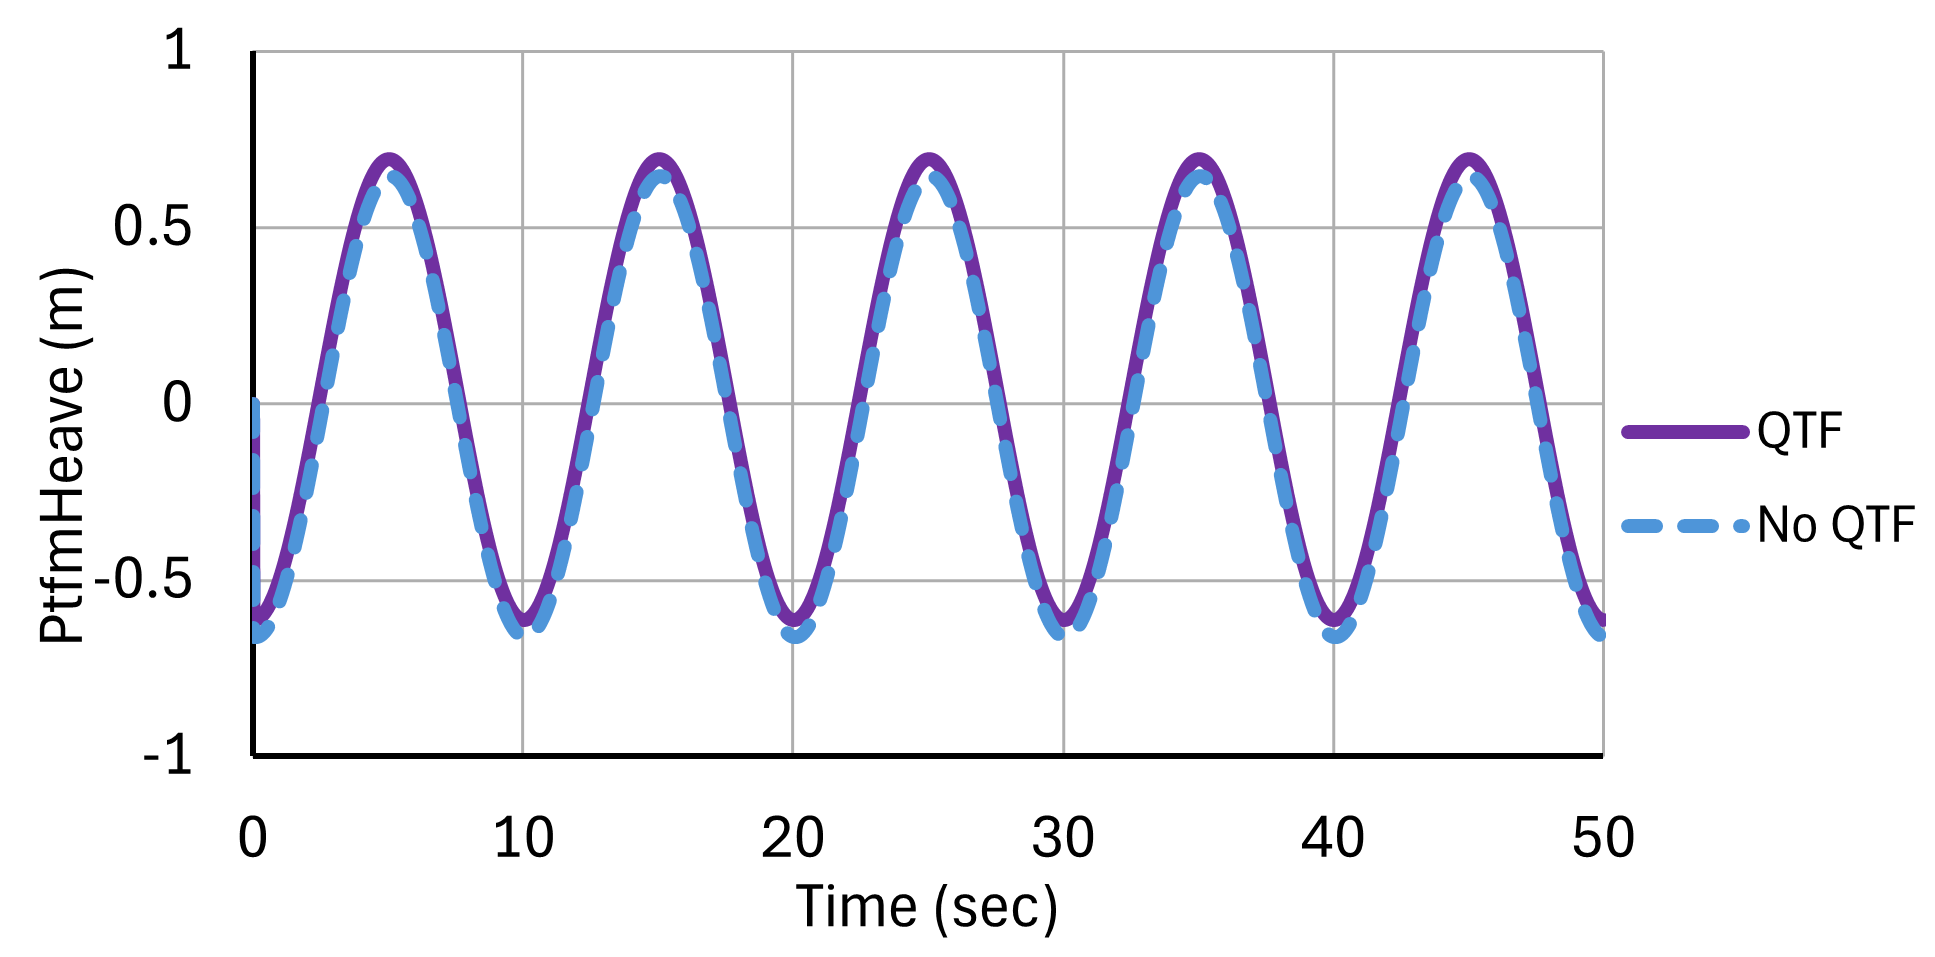
\includegraphics[width=1\textwidth]{2.1_heave_mine.png}
        \caption{\small Heave response}
        \label{fig:2.1_heave_mine}
    \end{minipage}
\end{figure}

\begin{figure}[H]
    \begin{minipage}{0.48\textwidth}
        \centering
        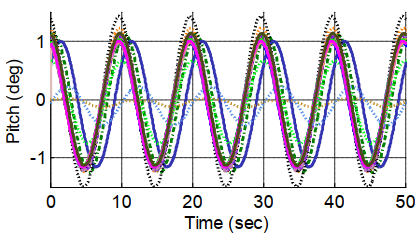
\includegraphics[width=1\textwidth]{2.1_pitch.png}
        \caption{\small Pitch response \cite{Robertson2014}}
        \label{fig:2.1_pitch}
    \end{minipage}
    \hfill
    \begin{minipage}{0.51\textwidth}
        \centering
        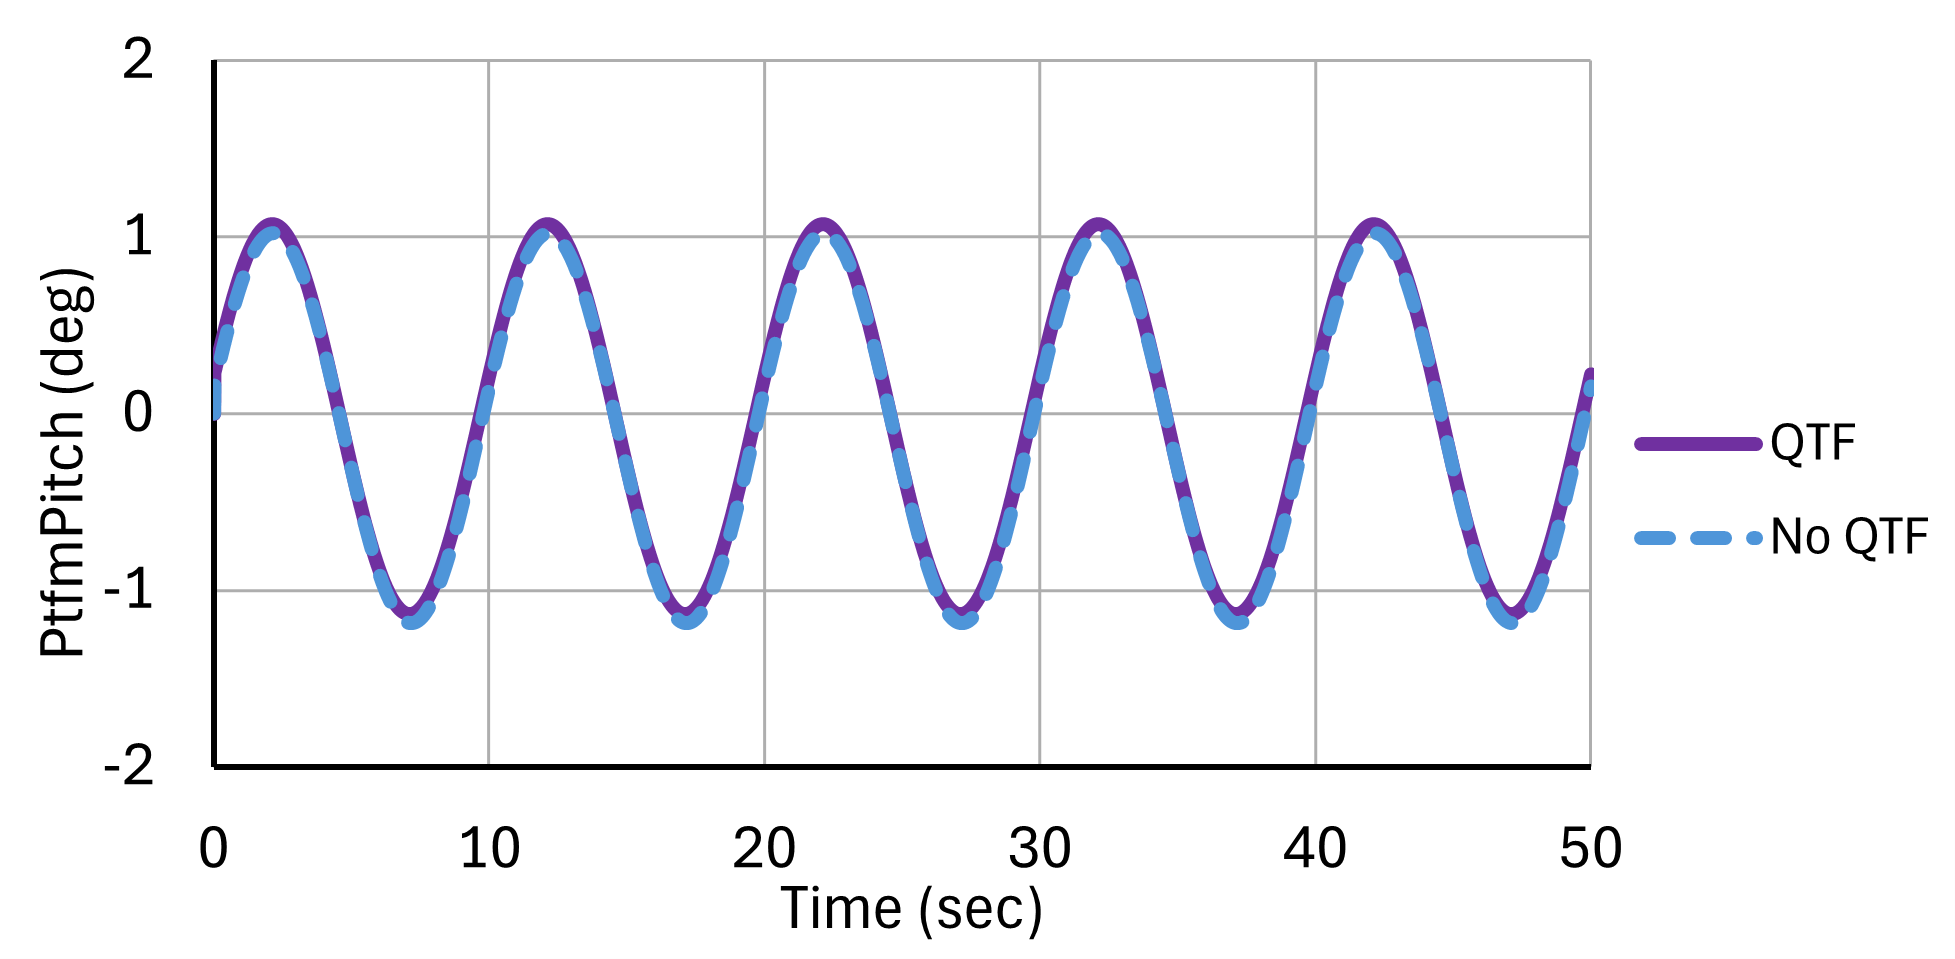
\includegraphics[width=1\textwidth]{2.1_pitch_mine.png}
        \caption{\small Pitch response}
        \label{fig:2.1_pitch_mine}
    \end{minipage}
\end{figure}

\begin{figure}[H]
    \begin{minipage}{0.48\textwidth}
        \centering
        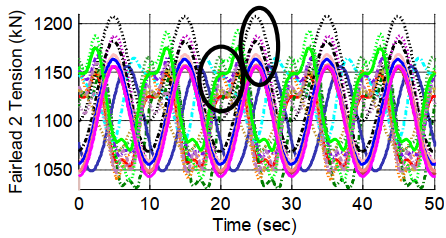
\includegraphics[width=1\textwidth]{2.1_fairten2.png}
        \caption{\small Fairlead 2 response \cite{Robertson2014}}
        \label{fig:2.1_fairten2}
    \end{minipage}
    \hfill
    \begin{minipage}{0.51\textwidth}
        \centering
        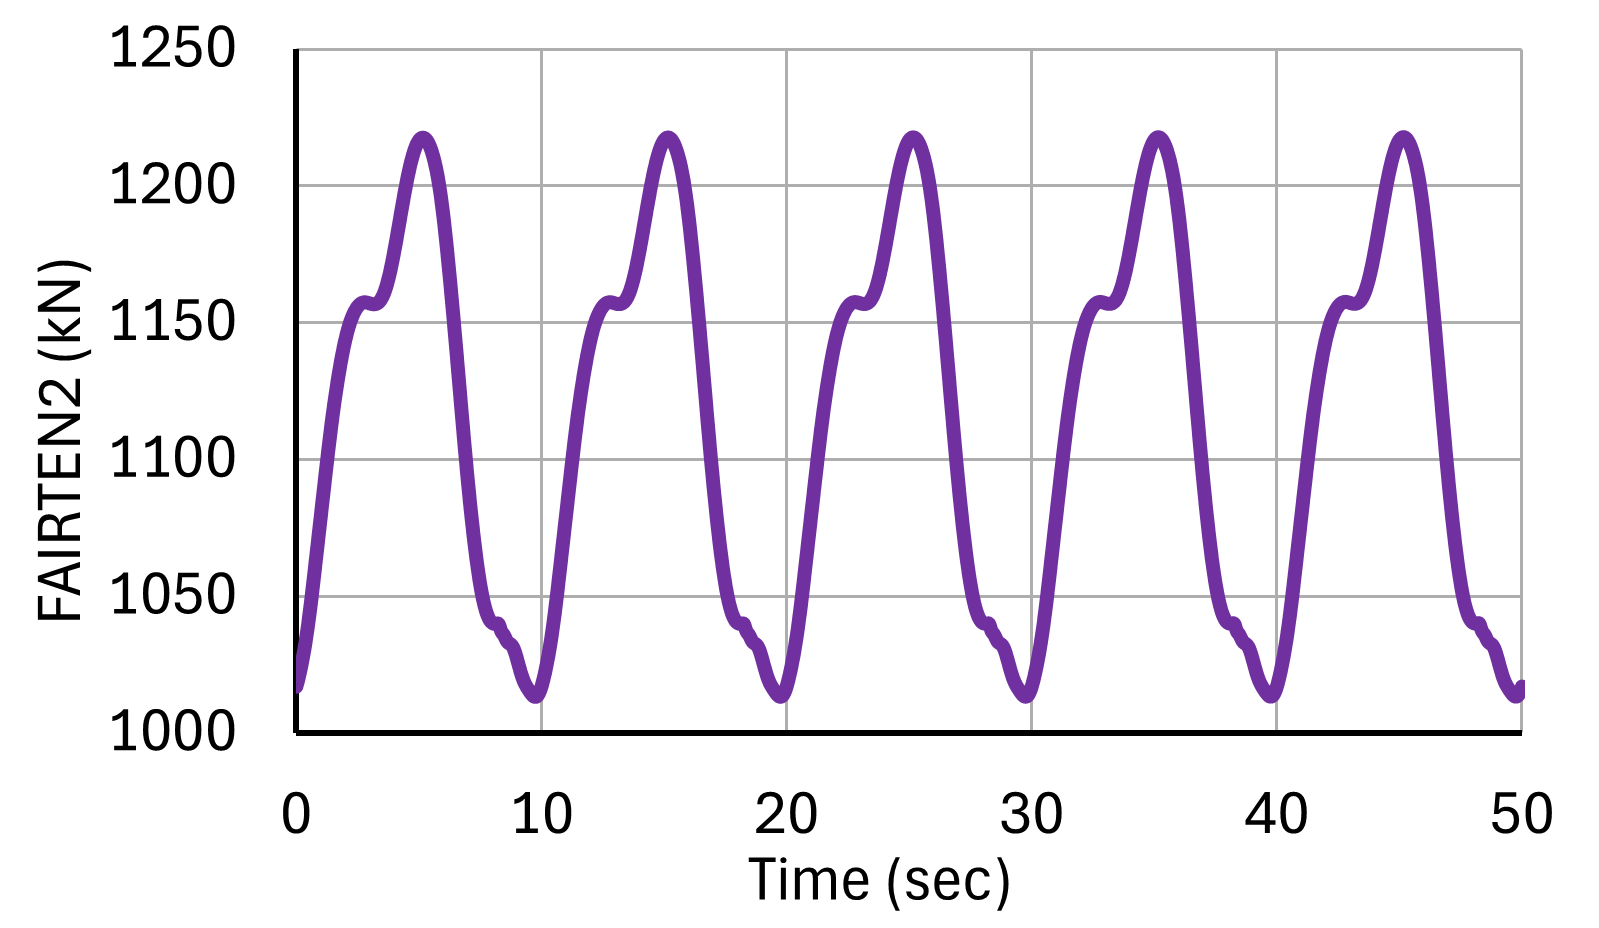
\includegraphics[width=0.95\textwidth]{2.1_fairten2_mine.png}
        \caption{\small Fairlead 2 response}
        \label{fig:2.1_fairten2_mine}
    \end{minipage}
\end{figure}

\subsubsection{Load Case 2.2}

\hspace{0.5cm}Load case 2.2 analyzes the platform's response to irregular waves, examining surge motion, pitch motion, and tower bending moment. The reference study shows significant variation in average responses between participants (\autoref{fig:2.2}), caused by different modeling approaches, particularly whether drift effects were included. Results processed through BEMRosetta compare simulations with and without quadratic transfer function (QTF) analysis (Figures~\ref{fig:2.2_surge}--\ref{fig:2.2_twr}). 

\begin{figure}[H]
    \centering
    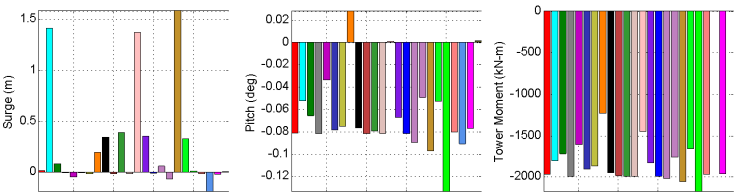
\includegraphics[width=1\textwidth]{2.2.png}
    \caption{\small Average responses to irregular waves \cite{Robertson2014}}
    \label{fig:2.2}
\end{figure}

\begin{figure}[H]
    \centering
    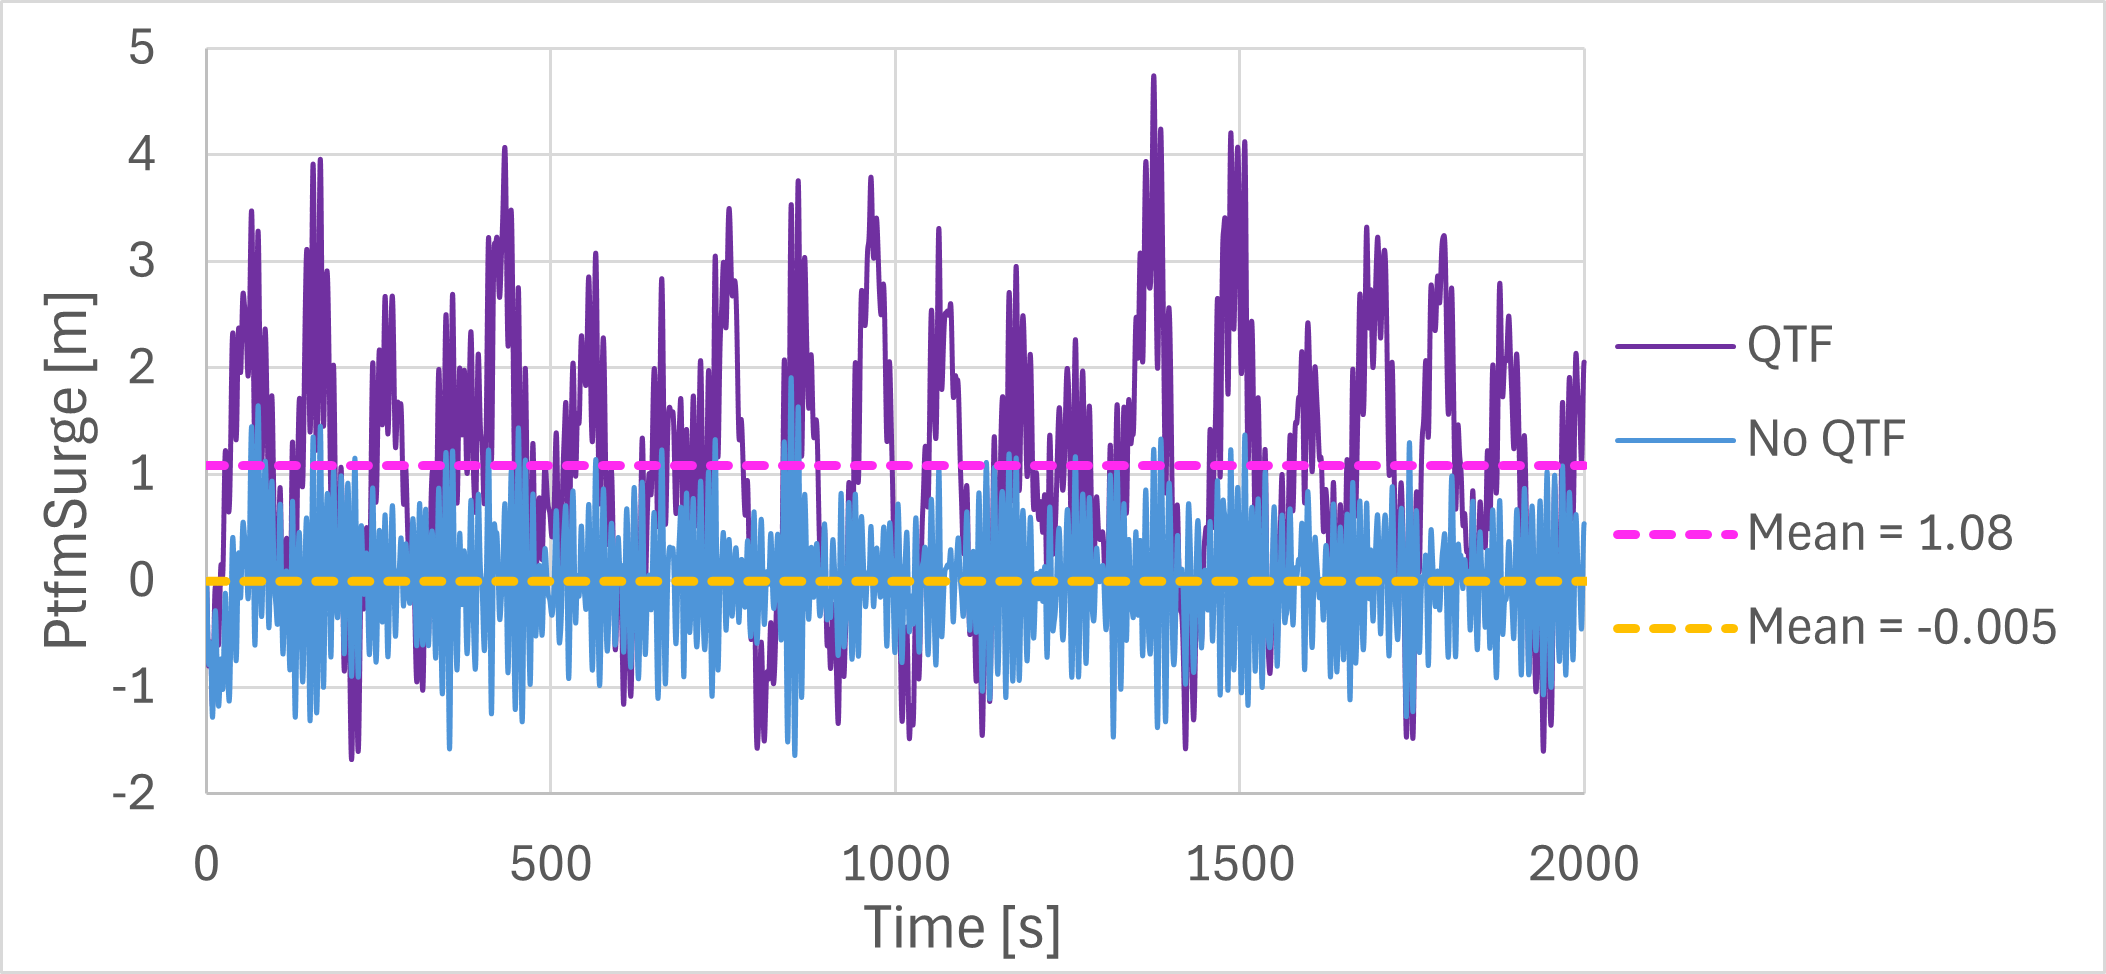
\includegraphics[width=0.78\textwidth]{2.2_surge.png}
    \caption{\small Surge response to irregular waves}
    \label{fig:2.2_surge}
\end{figure}

\begin{figure}[H]
    \centering
    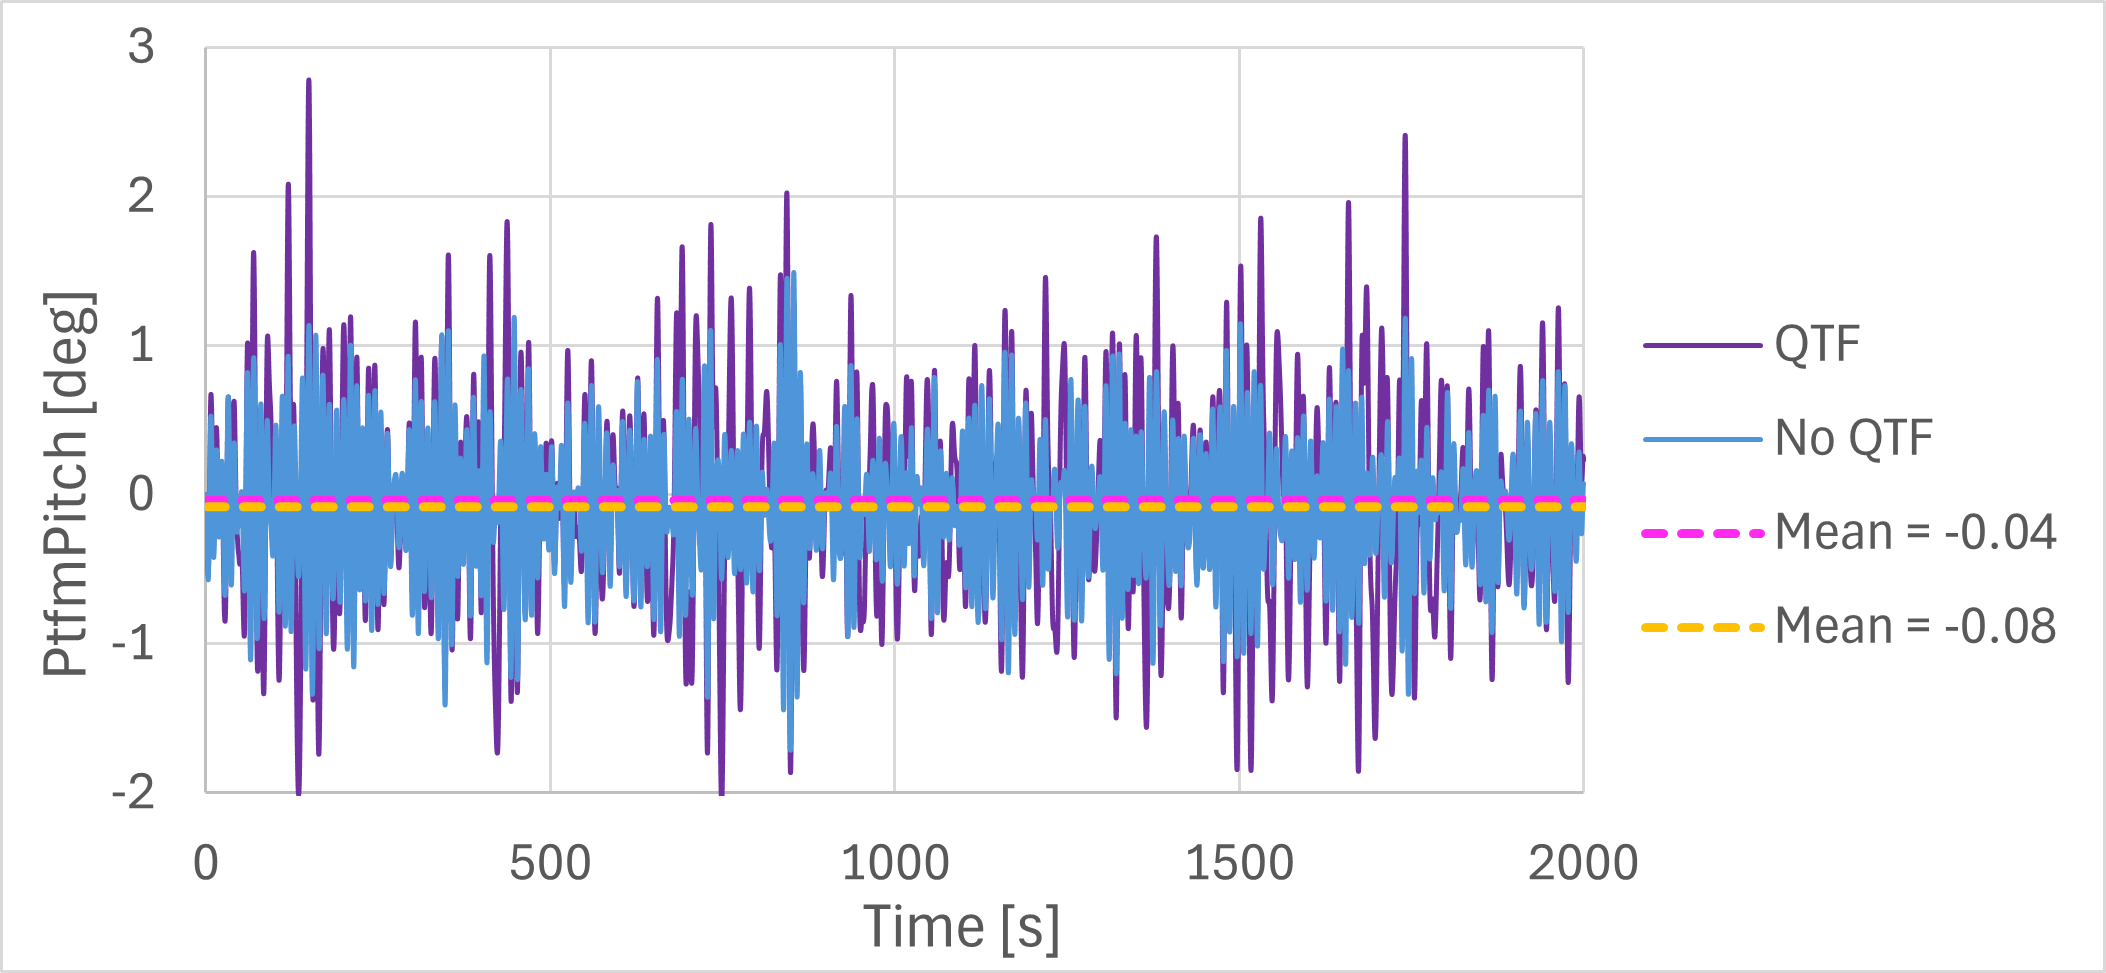
\includegraphics[width=0.78\textwidth]{2.2_pitch.png}
    \caption{\small Pitch response to irregular waves}
    \label{fig:2.2_pitch}
\end{figure}

\begin{figure}[H]
    \centering
    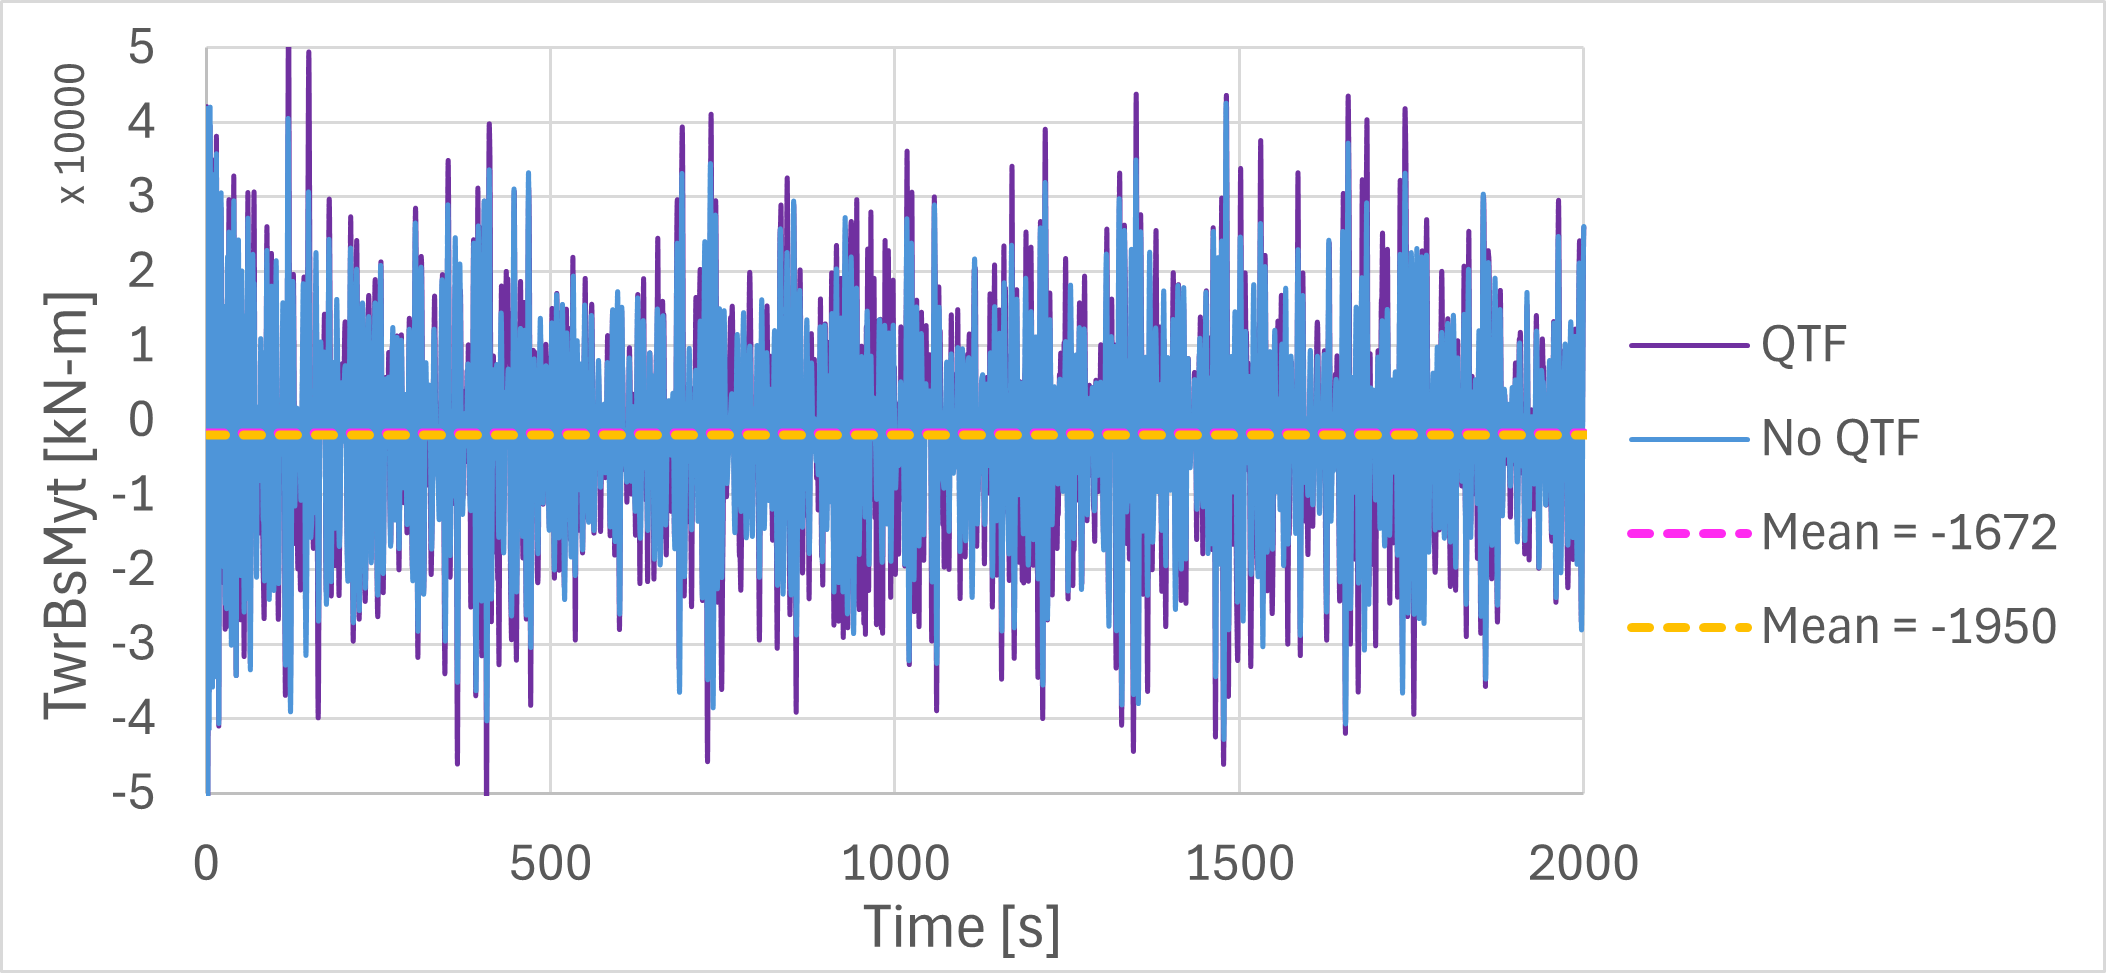
\includegraphics[width=0.78\textwidth]{2.2_twr.png}
    \caption{\small Tower bending response to irregular waves (fore/aft direction)}
    \label{fig:2.2_twr}
\end{figure}

Similar to load case 2.1, the results show that the surge motion is highly sensitive to second-order drift effects. In contrast, pitch motion and tower bending moment show minimal changes. The consistent patterns observed in this analysis match well with participant results when accounting for each study's specific modeling choices.

\subsubsection{Load Case 2.4 \& 2.5}
\hspace{0.5cm}The load cases 2.4 and 2.5 were not analyzed in detail in the reference study. However, they were included in this analysis to assess the impact of second-order drift effects on the platform's response to the combination of wave and current effects and extreme wave conditions.

Load case 2.4 represents operational conditions with regular waves that have a significant wave height of 6 meters and a wave period of 10 seconds, along with a surface current of 0.5 meters per second. Load case 2.5 examines extreme conditions characterized by irregular waves with a significant wave height of 50 meters and a wave period of 19.2 seconds.

\begin{figure}[H]
    \begin{minipage}{0.49\textwidth}
        \centering
        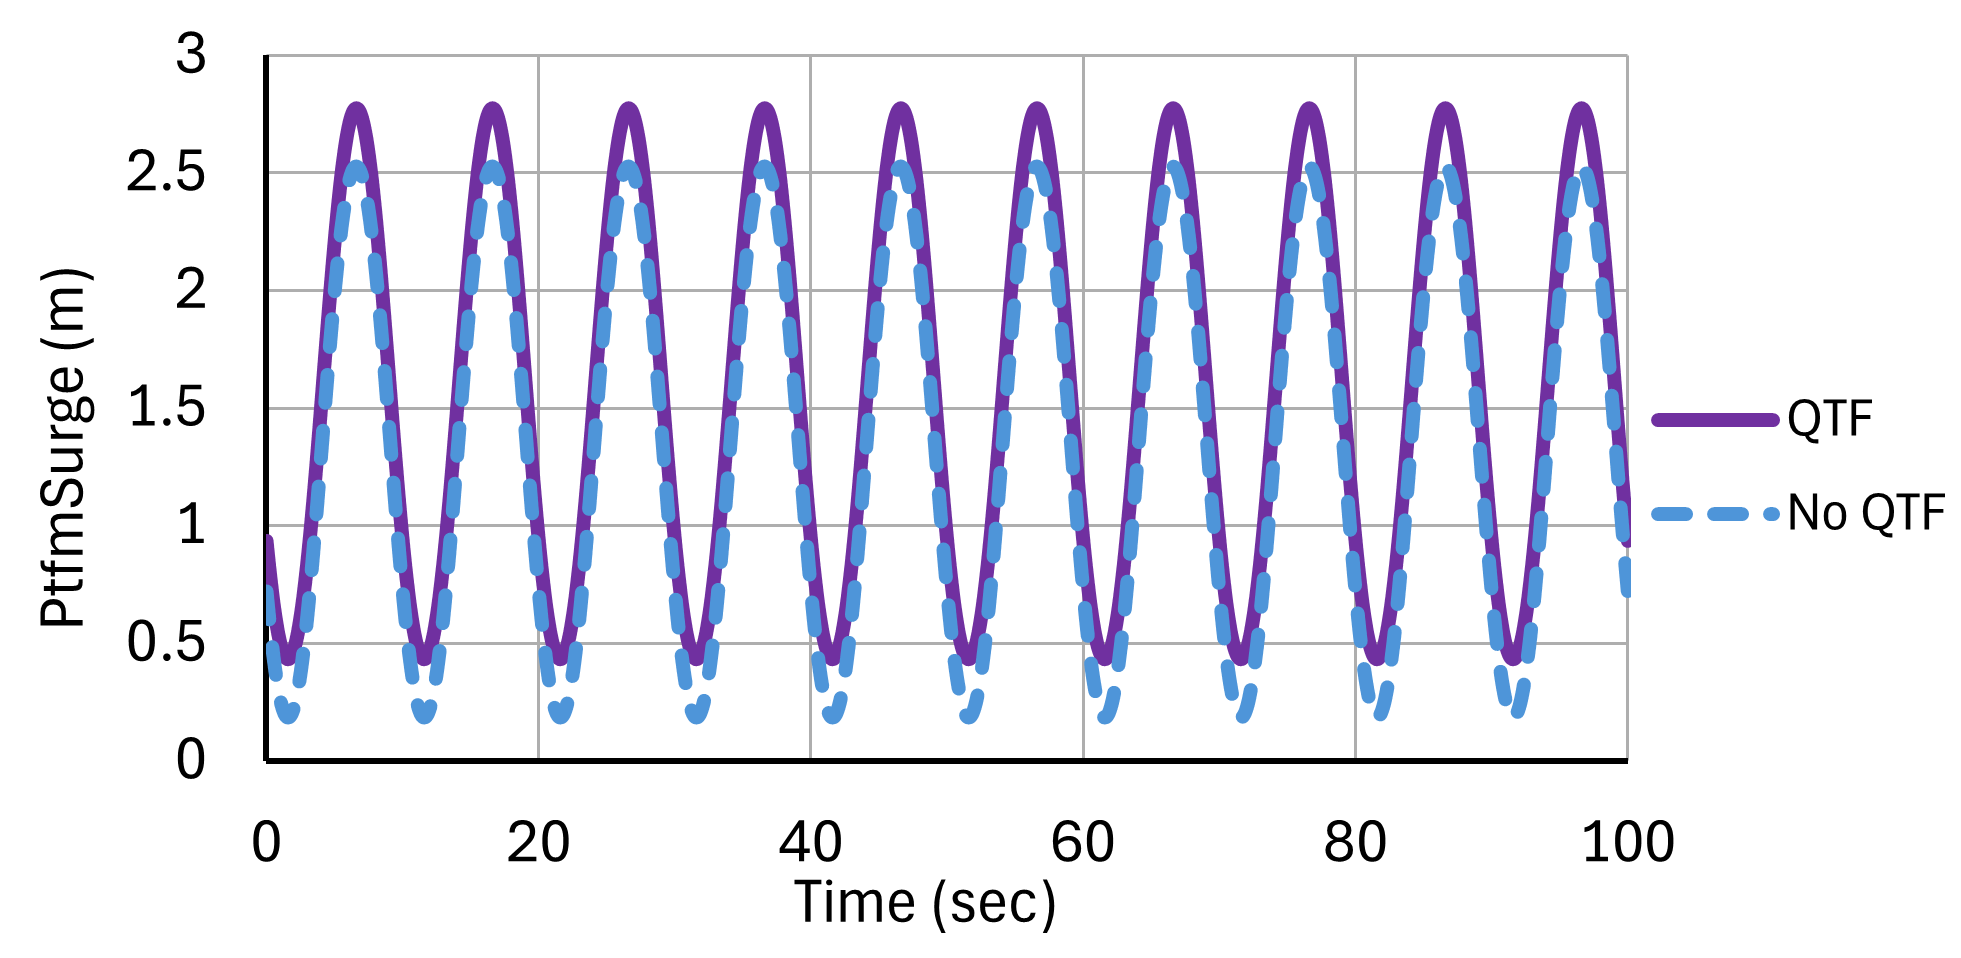
\includegraphics[width=1\textwidth]{2.4_surge.png}
        \caption{\small Surge response for load case 2.4} 
        \label{fig:2.4_surge}
    \end{minipage}
    \hfill
    \begin{minipage}{0.49\textwidth}
        \centering
        \vspace{-0.3cm}
        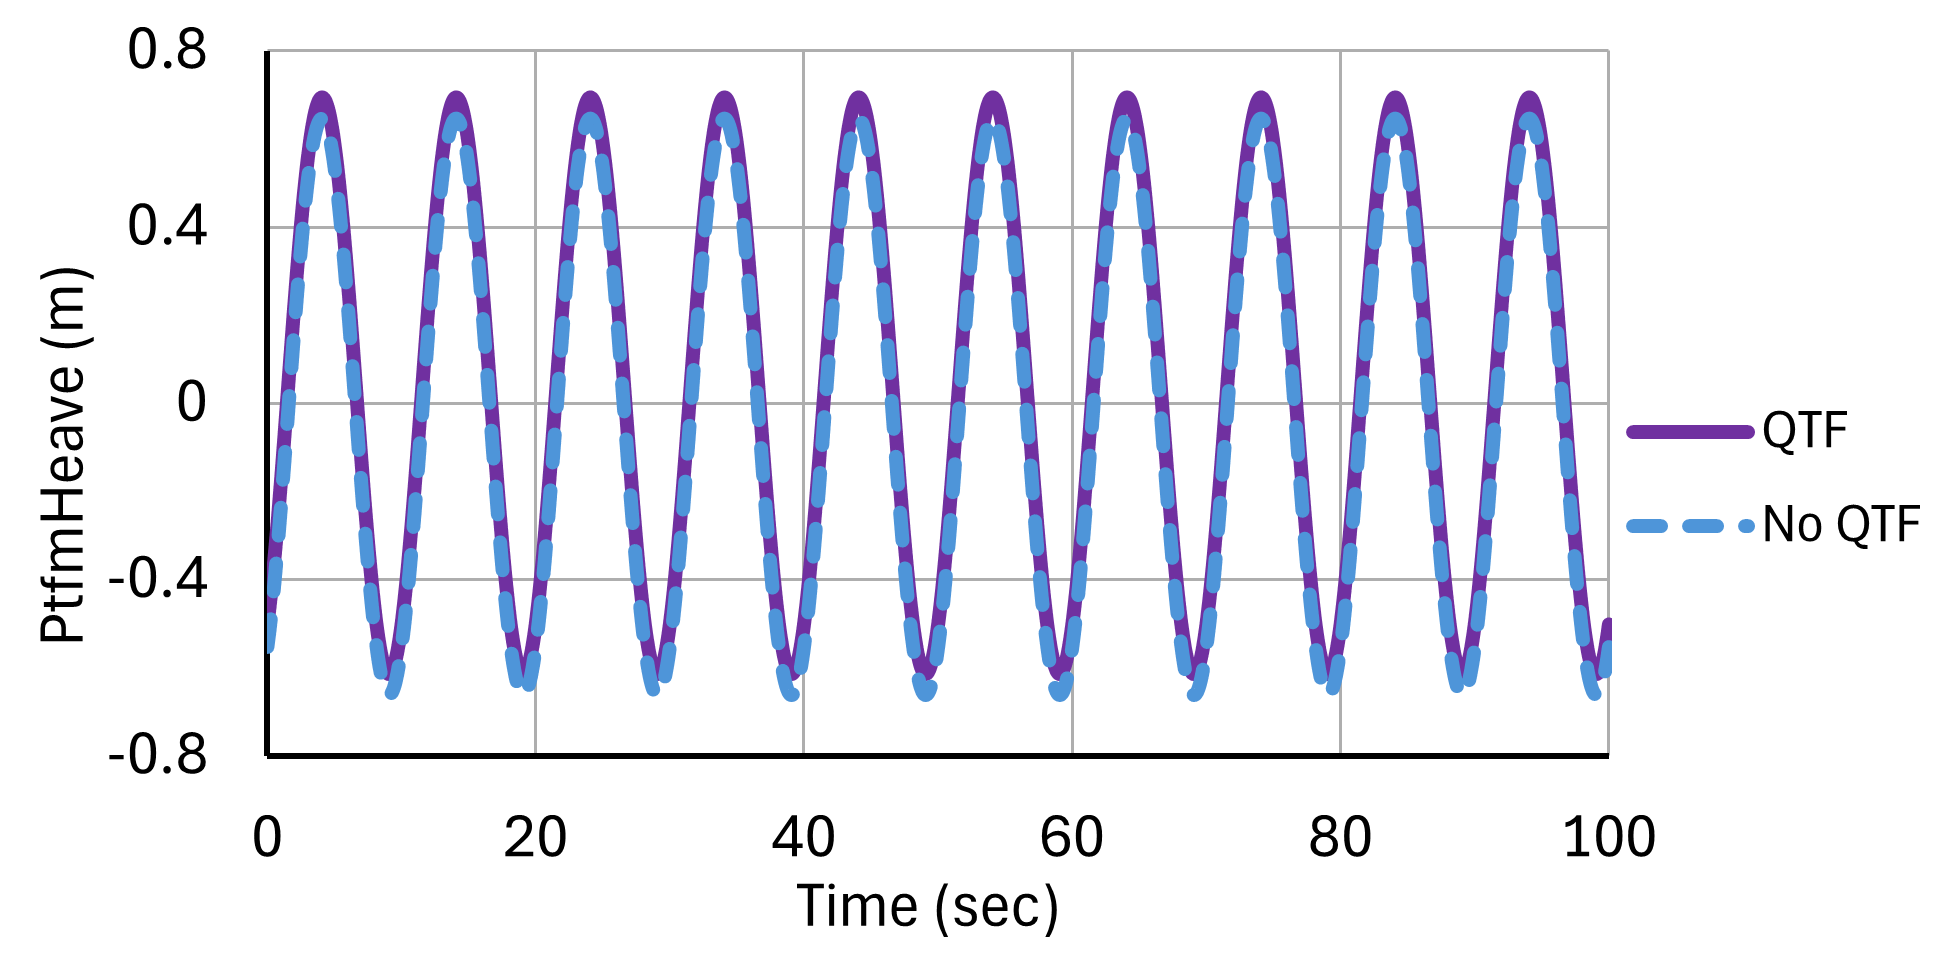
\includegraphics[width=1\textwidth]{2.4_heave.png}
        \caption{\small Heave response for load case 2.4}
        \label{fig:2.4_heave}
    \end{minipage}
\end{figure}

\begin{figure}[H]
    \begin{minipage}{0.49\textwidth}
        \centering
        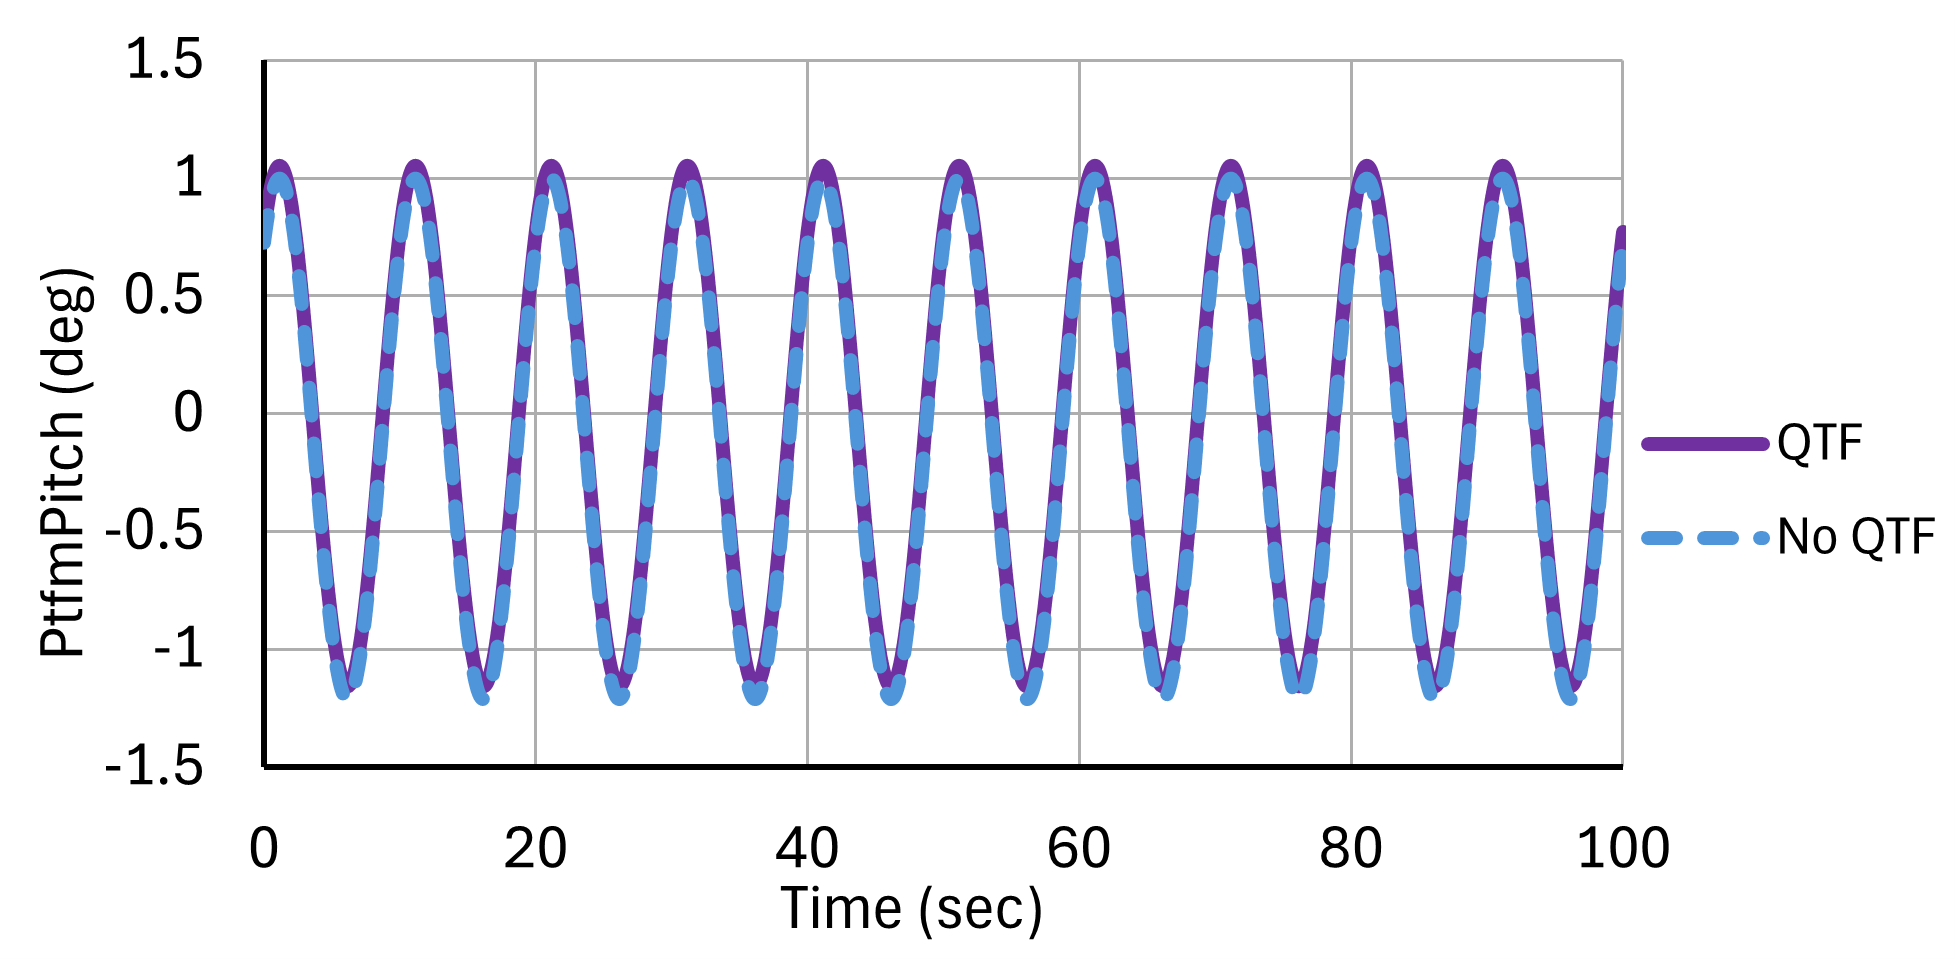
\includegraphics[width=1\textwidth]{2.4_pitch.png}
        \caption{\small Pitch response for load case 2.4} 
        \label{fig:2.4_pitch}
    \end{minipage}
    \hfill
    \begin{minipage}{0.49\textwidth}
        \centering
        \vspace{-0.3cm}
        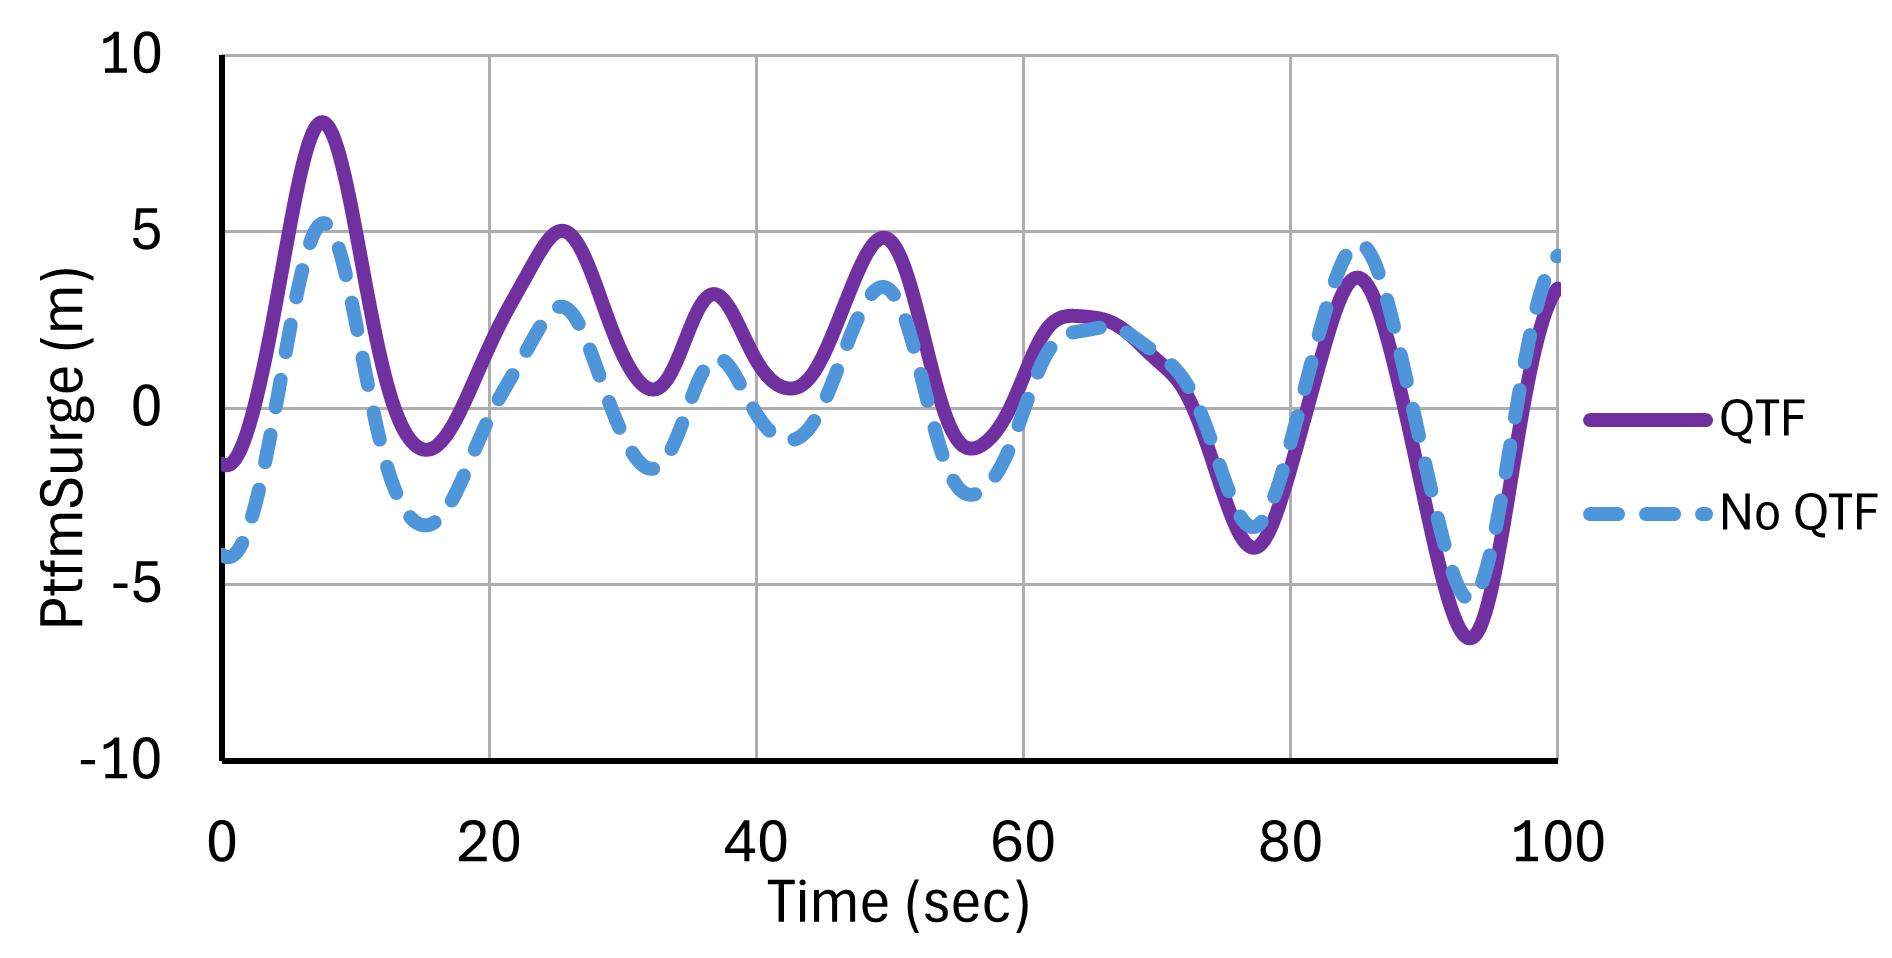
\includegraphics[width=1\textwidth]{2.5_surge.png}
        \caption{\small Surge response for load case 2.5}
        \label{fig:2.5_surge}
    \end{minipage}
\end{figure}

\begin{figure}[H]
    \begin{minipage}{0.49\textwidth}
        \centering
        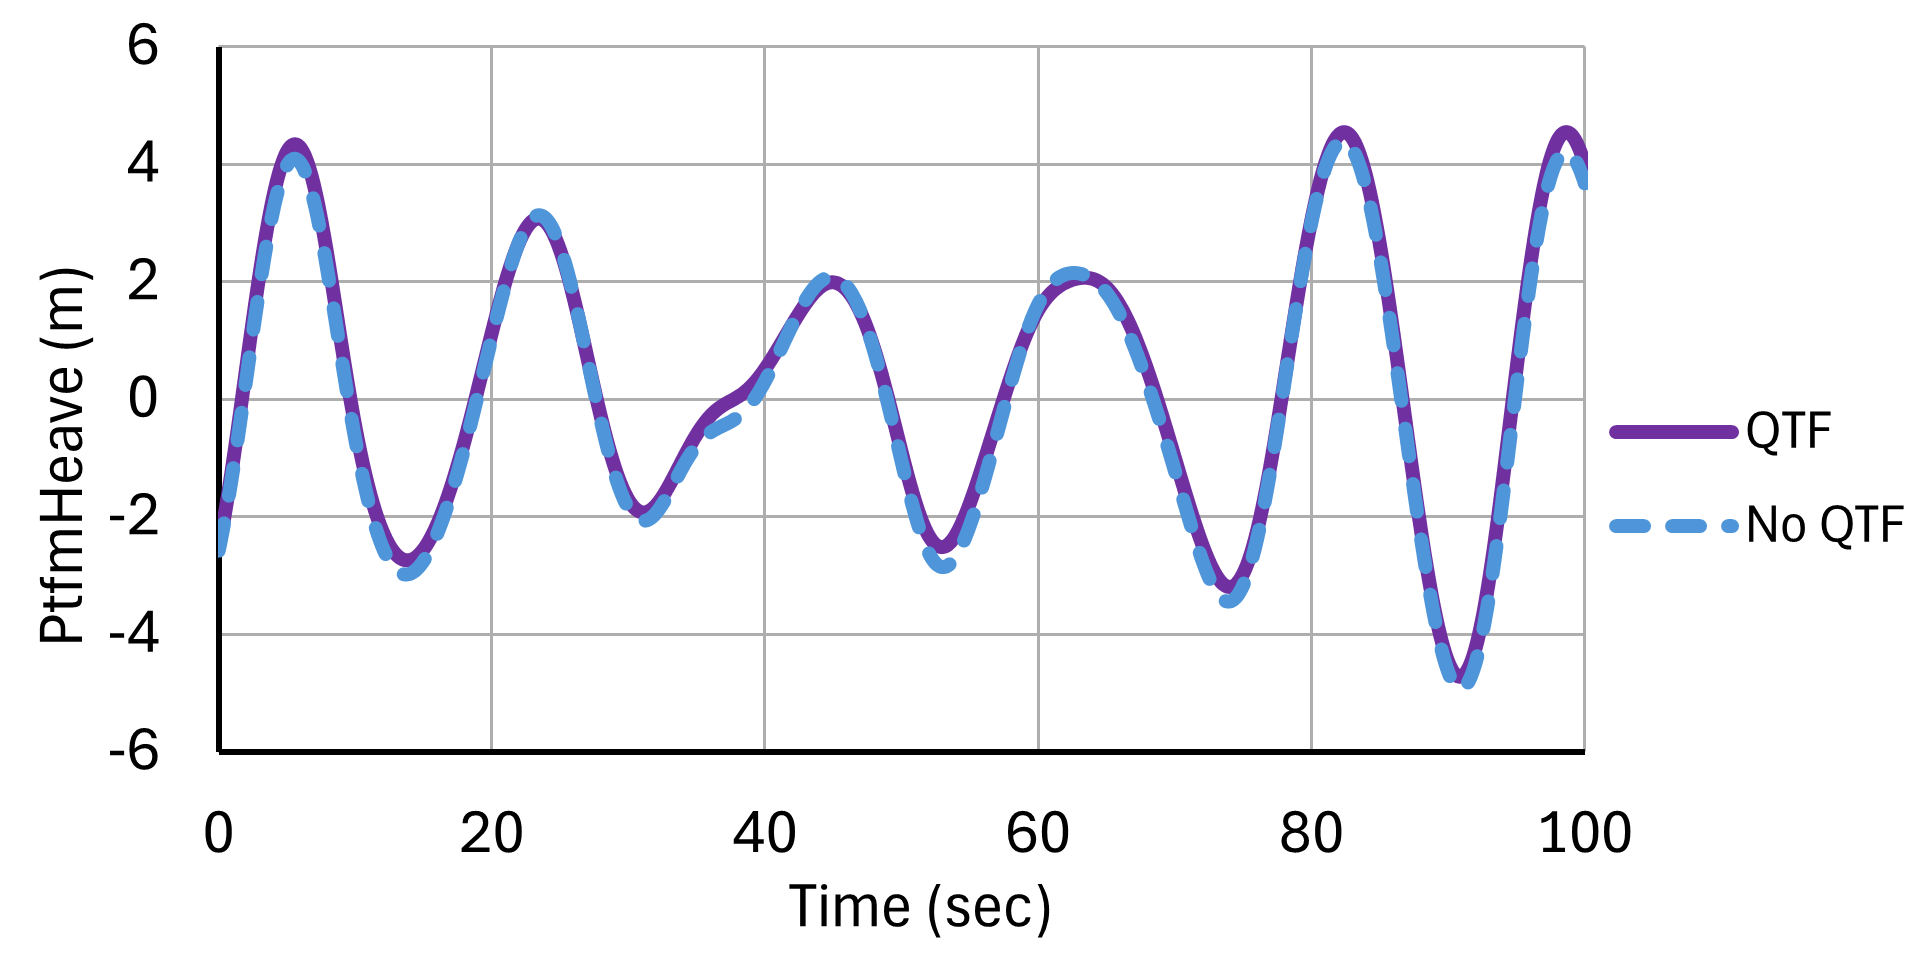
\includegraphics[width=1\textwidth]{2.5_heave.png}
        \caption{\small Heave response for load case 2.5}
        \label{fig:2.5_heave}
    \end{minipage}
    \hfill
    \begin{minipage}{0.49\textwidth}
        \centering
        \vspace{-0.3cm}
        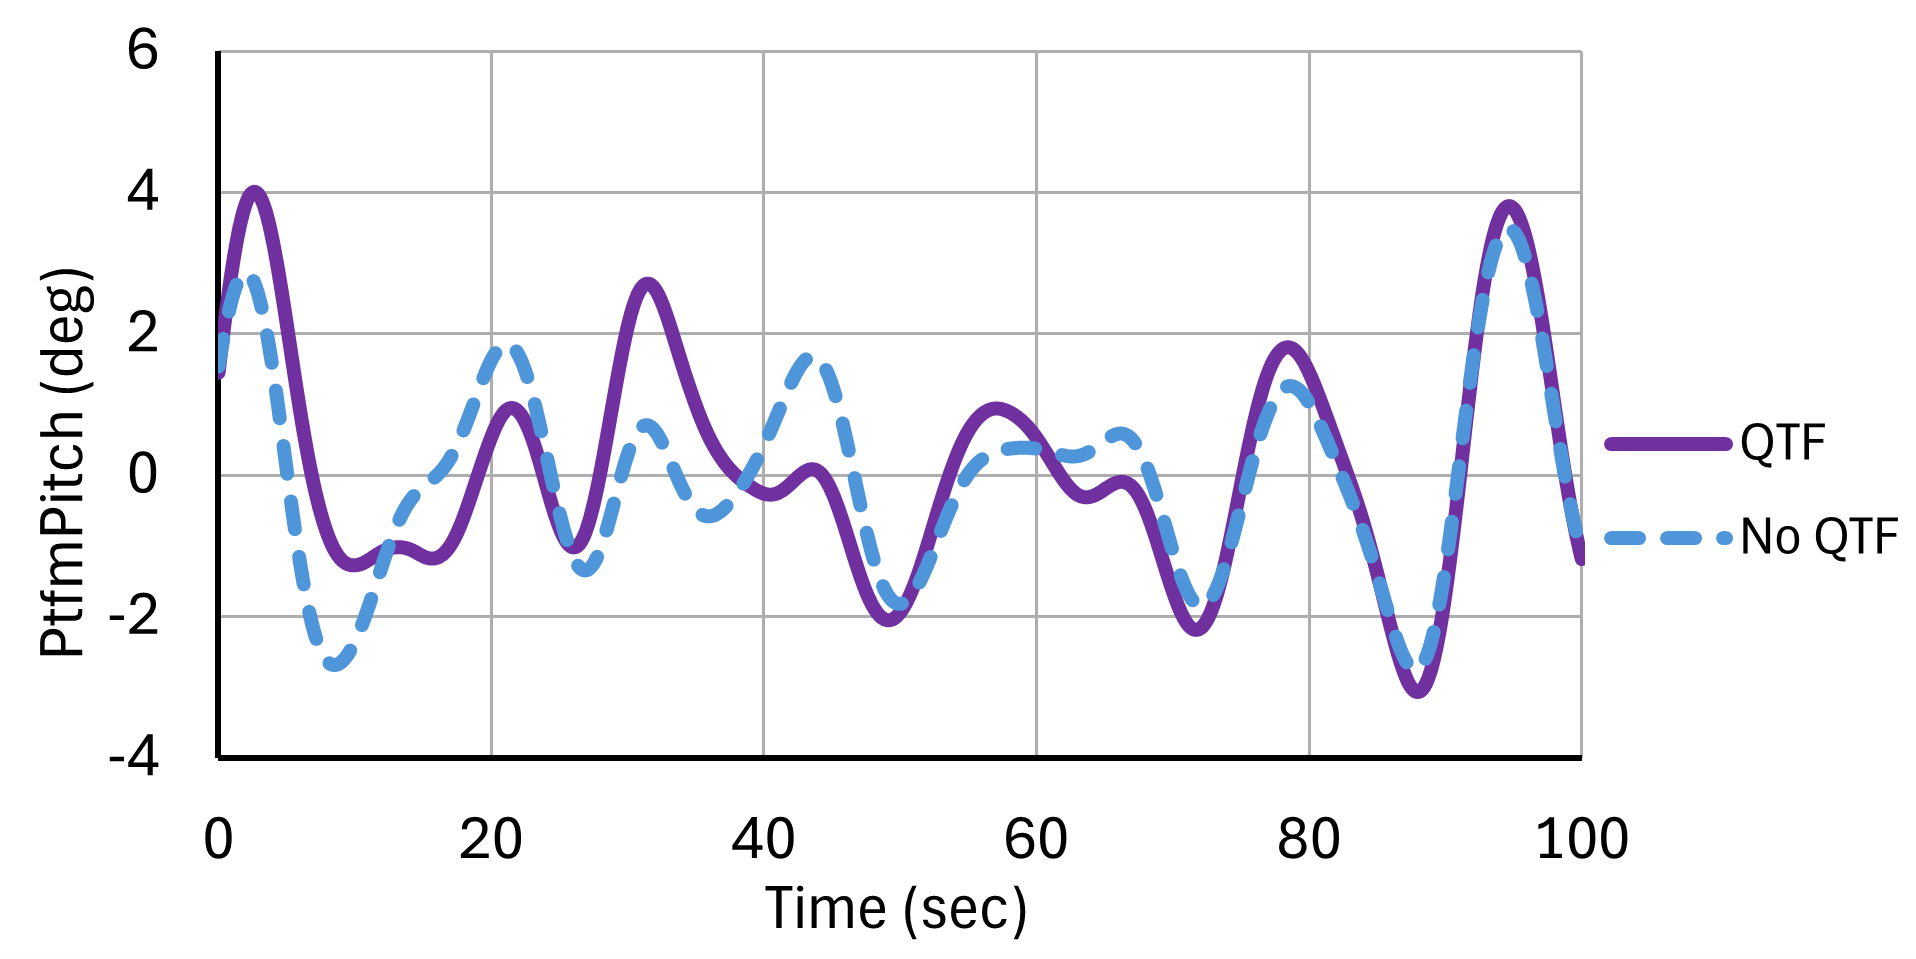
\includegraphics[width=1\textwidth]{2.5_pitch.png}
        \caption{\small Pitch response for load case 2.5}
        \label{fig:2.5_pitch}
    \end{minipage}
\end{figure}

The comparative results, presented in Figures~\ref{fig:2.4_surge}--\ref{fig:2.5_pitch}, demonstrate that second-order drift effects impact platform response. Surge and pitch motions show higher sensitivity to these effects, particularly under the extreme wave conditions of load case 2.5. Heave motion, consistent with findings from previous load cases, remains relatively unaffected by the inclusion of second-order analysis.

\subsubsection{Load Case 2.6}
\hspace*{0.5cm}Load case 2.6 analyzes the platform's response to banded white noise to obtain Response Amplitudes Operators (RAOs) for the platform. RAOs represent the ratio of a system's response to the wave amplitude caused by wave excitation \cite{RAO}. For this study, the RAOs were calculated through dividing the each response PSD to the wave elevation PSD in the banded white-noise spectrum between 0.05 and 0.25 Hz and compared to the results from the reference study for both QTF (purple plot) and non-QTF (green plot) cases (Figures~\ref{fig:w_t_t_p}--\ref{fig:2.6_pitch_mine}).

\begin{figure}[H]
    \centering
    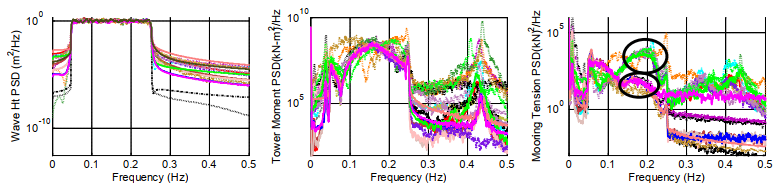
\includegraphics[width=1\textwidth]{w_t_t_p.png}
    \caption{\small Wave elevation, tower bending, and mooring tension PSD \cite{Robertson2014}}
    \label{fig:w_t_t_p}
\end{figure}

\begin{figure}[H]
    \centering
    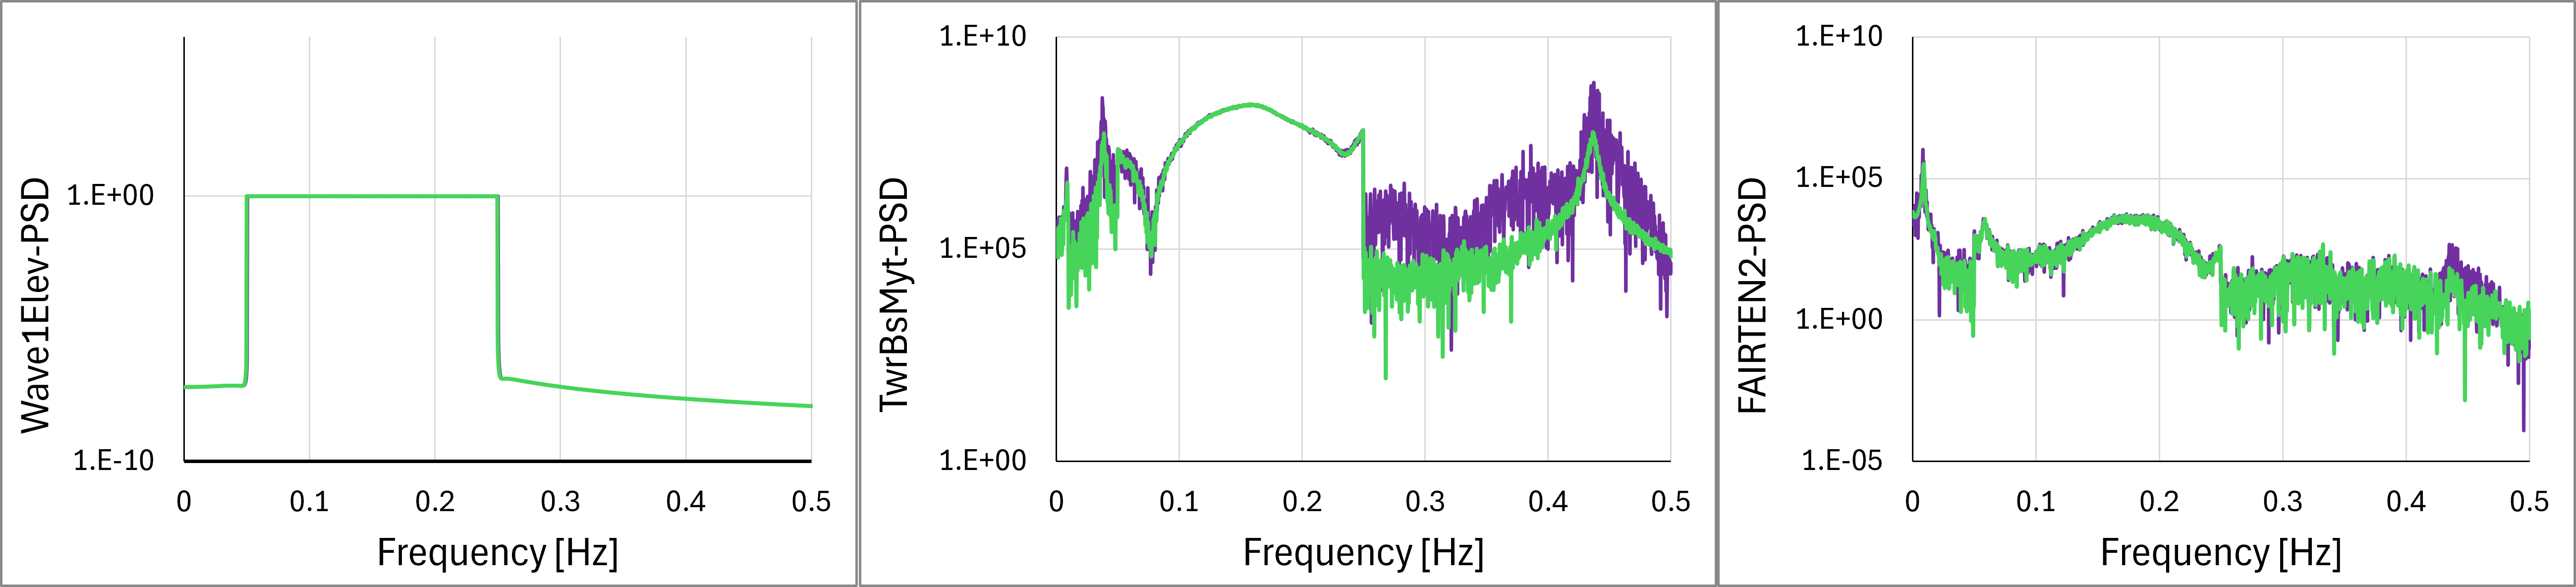
\includegraphics[width=1\textwidth]{wave_twr_ten_psd.png}
    \caption{\small Wave elevation, tower bending, and mooring tension PSD}
    \label{fig:w_t_t_p_mine}
\end{figure}

\begin{figure}[H]
    \centering
    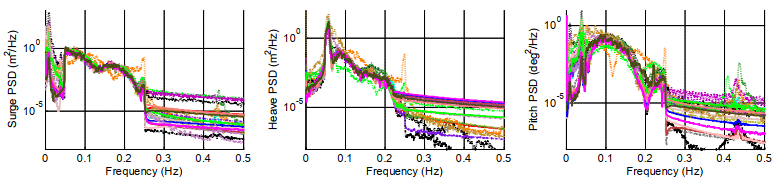
\includegraphics[width=1\textwidth]{s_h_p_p.png}
    \caption{\small Sugre, heave, and pitch PSD \cite{Robertson2014}}
    \label{fig:s_h_p_p}
\end{figure}

\begin{figure}[H]
    \centering
    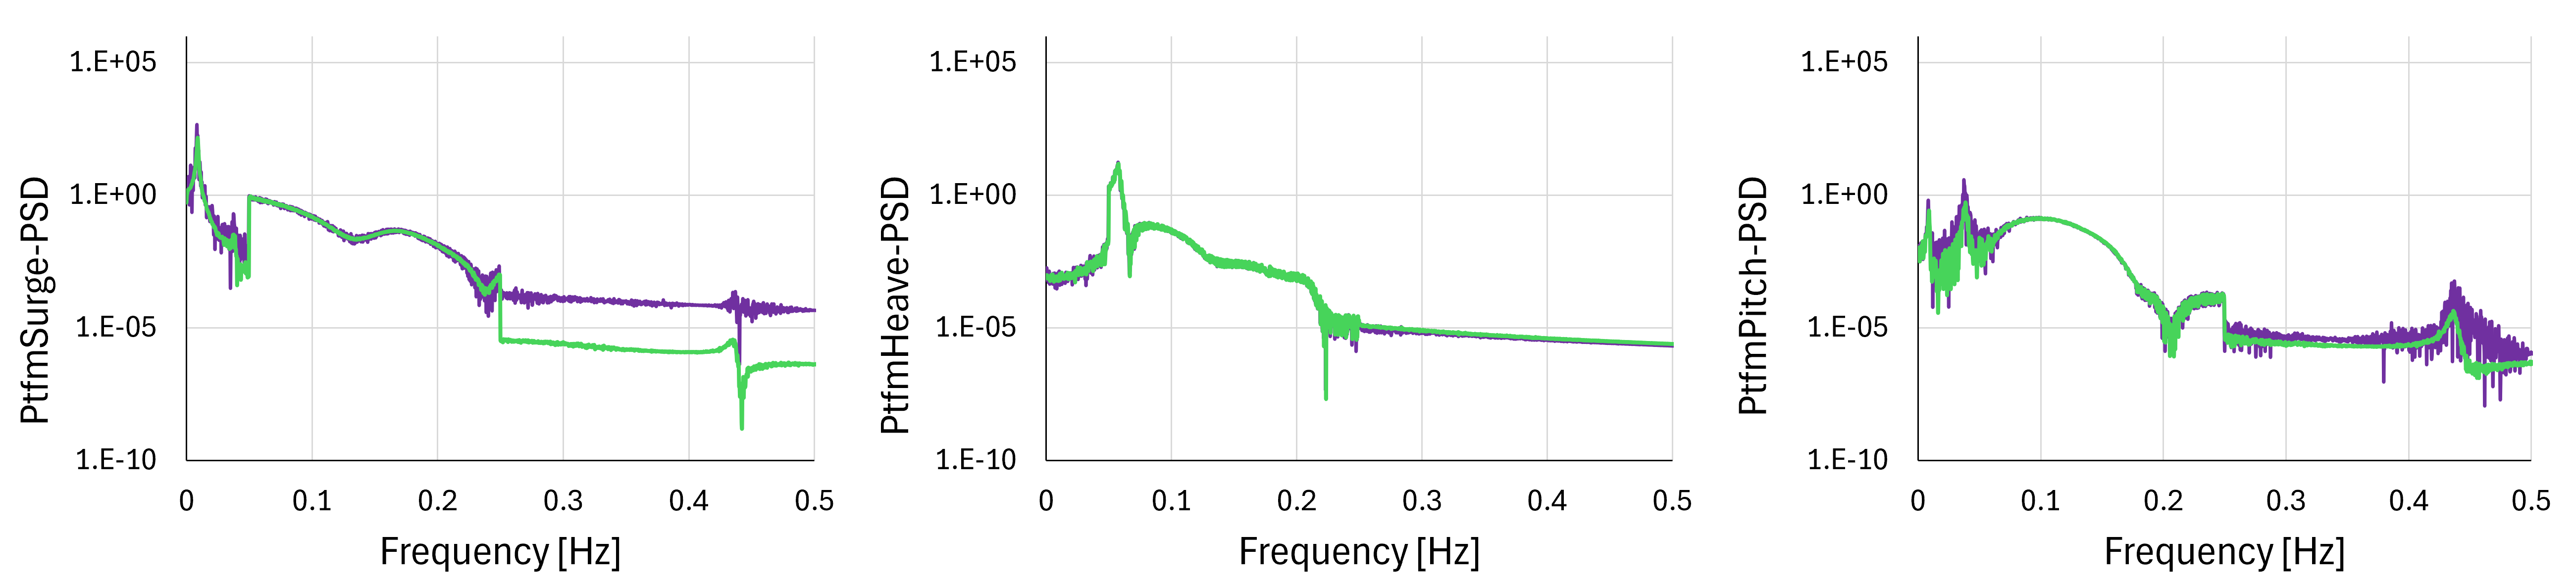
\includegraphics[width=1\textwidth]{sur_hea_pit_psd.png}
    \caption{\small Sugre, heave, and pitch PSD}
    \label{fig:s_h_p_p_mine}
\end{figure}

\begin{figure}[H]
    \begin{minipage}{0.48\textwidth}
        \centering
        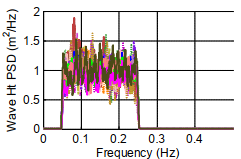
\includegraphics[width=1\textwidth]{2.6_wave.png}
        \caption{\small Wave elevation PSD \cite{Robertson2014}} 
        \label{fig:2.6_wave}
    \end{minipage}
    \hfill
    \begin{minipage}{0.51\textwidth}
        \centering
        \vspace{-0.3cm}
        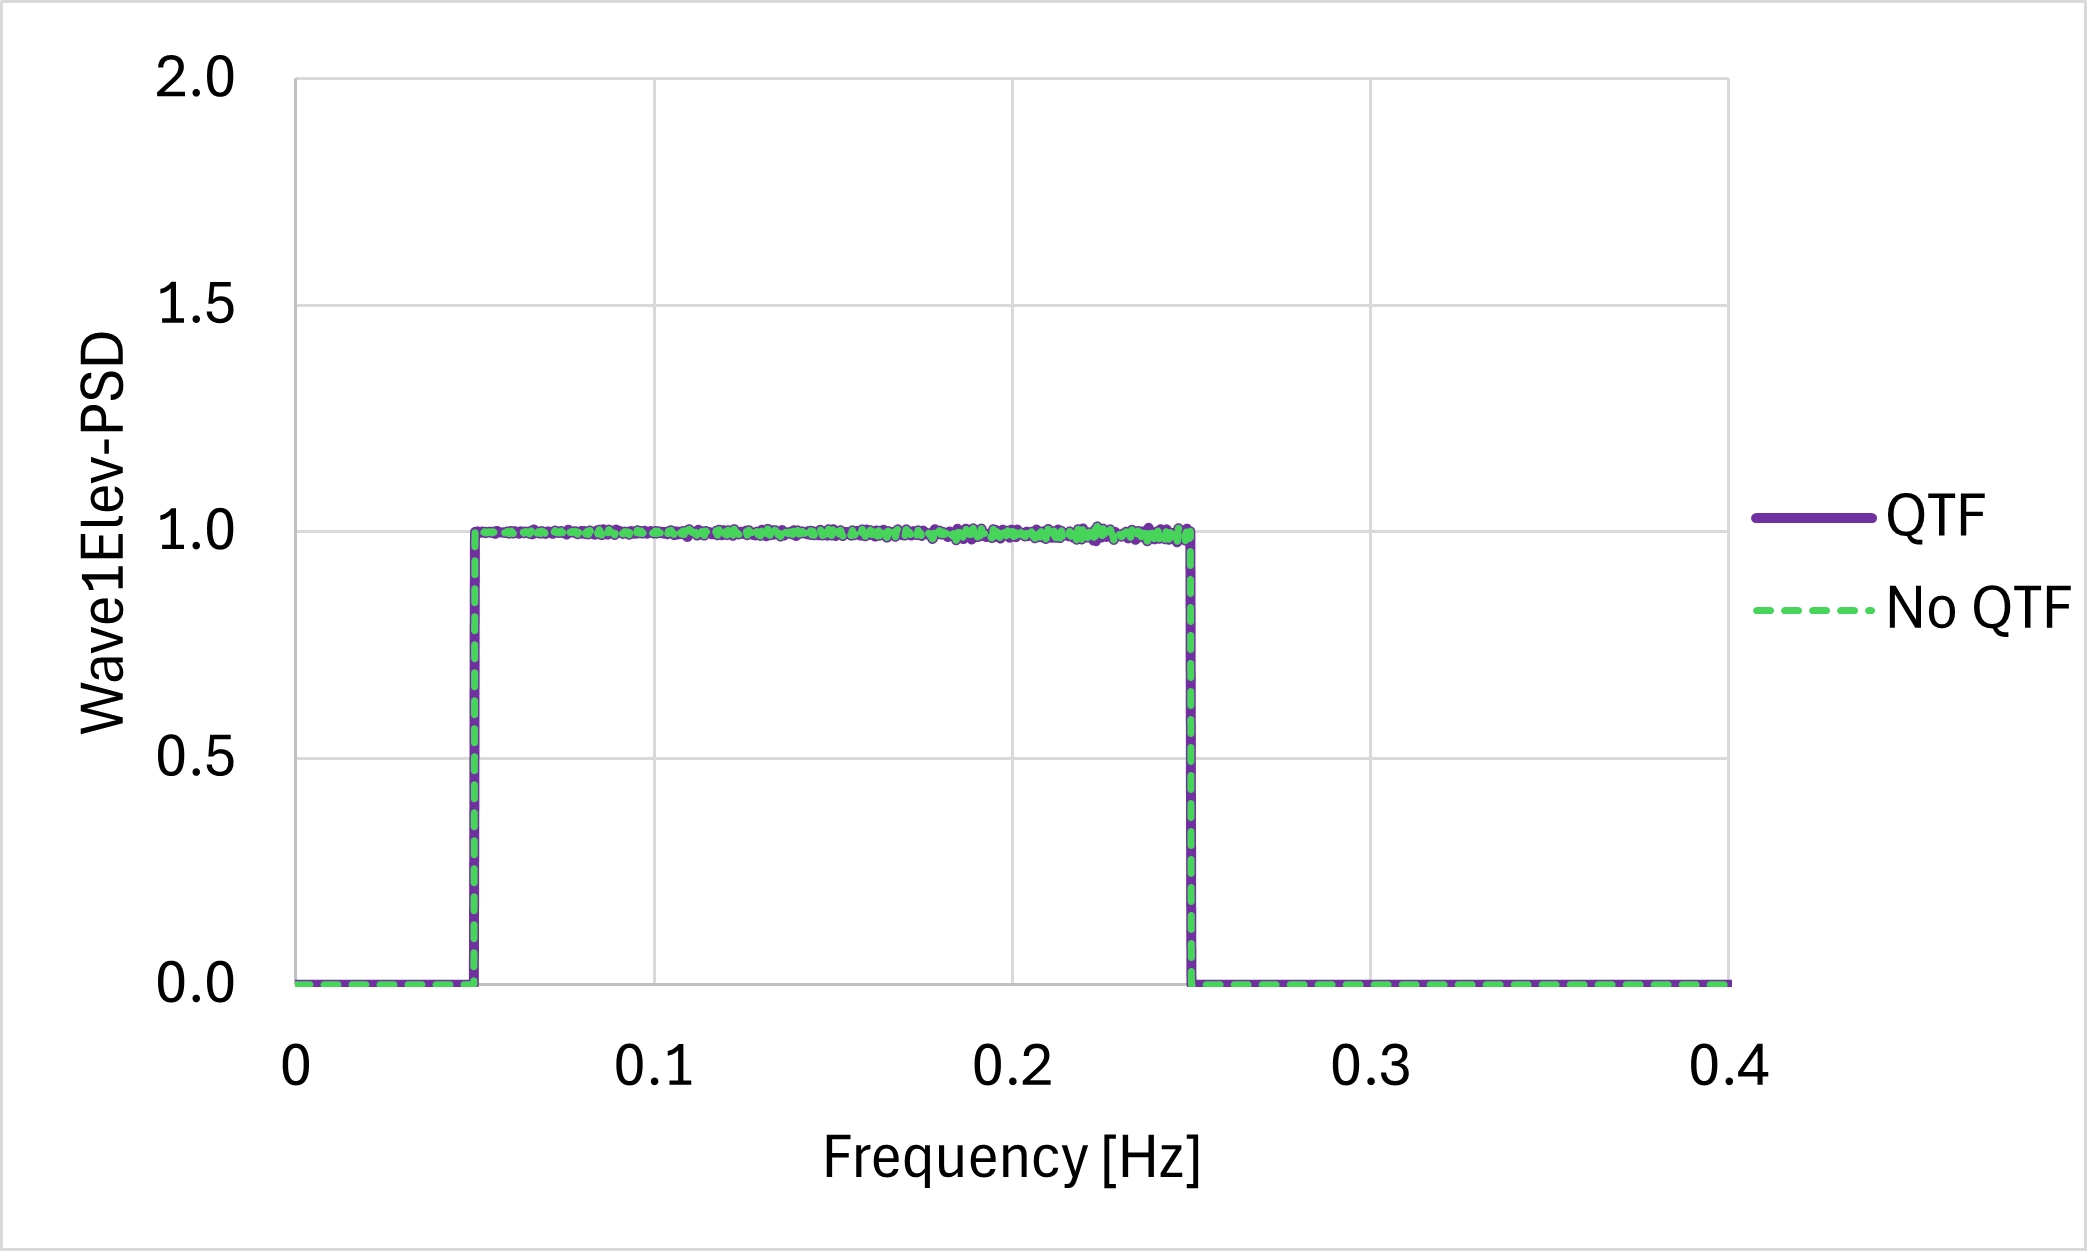
\includegraphics[width=1\textwidth]{2.6_wave_mine.png}
        \caption{\small Wave elevation PSD}
        \label{fig:2.6_wave_mine}
    \end{minipage}
\end{figure}

\begin{figure}[H]
    \begin{minipage}{0.48\textwidth}
        \centering
        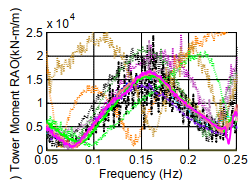
\includegraphics[width=0.95\textwidth]{2.6_twr.png}
        \caption{\small Tower bending moment RAO \cite{Robertson2014}}
        \label{fig:2.6_twr}
    \end{minipage}
    \hfill
    \begin{minipage}{0.5\textwidth}
        \centering
        \vspace{0.6cm}
        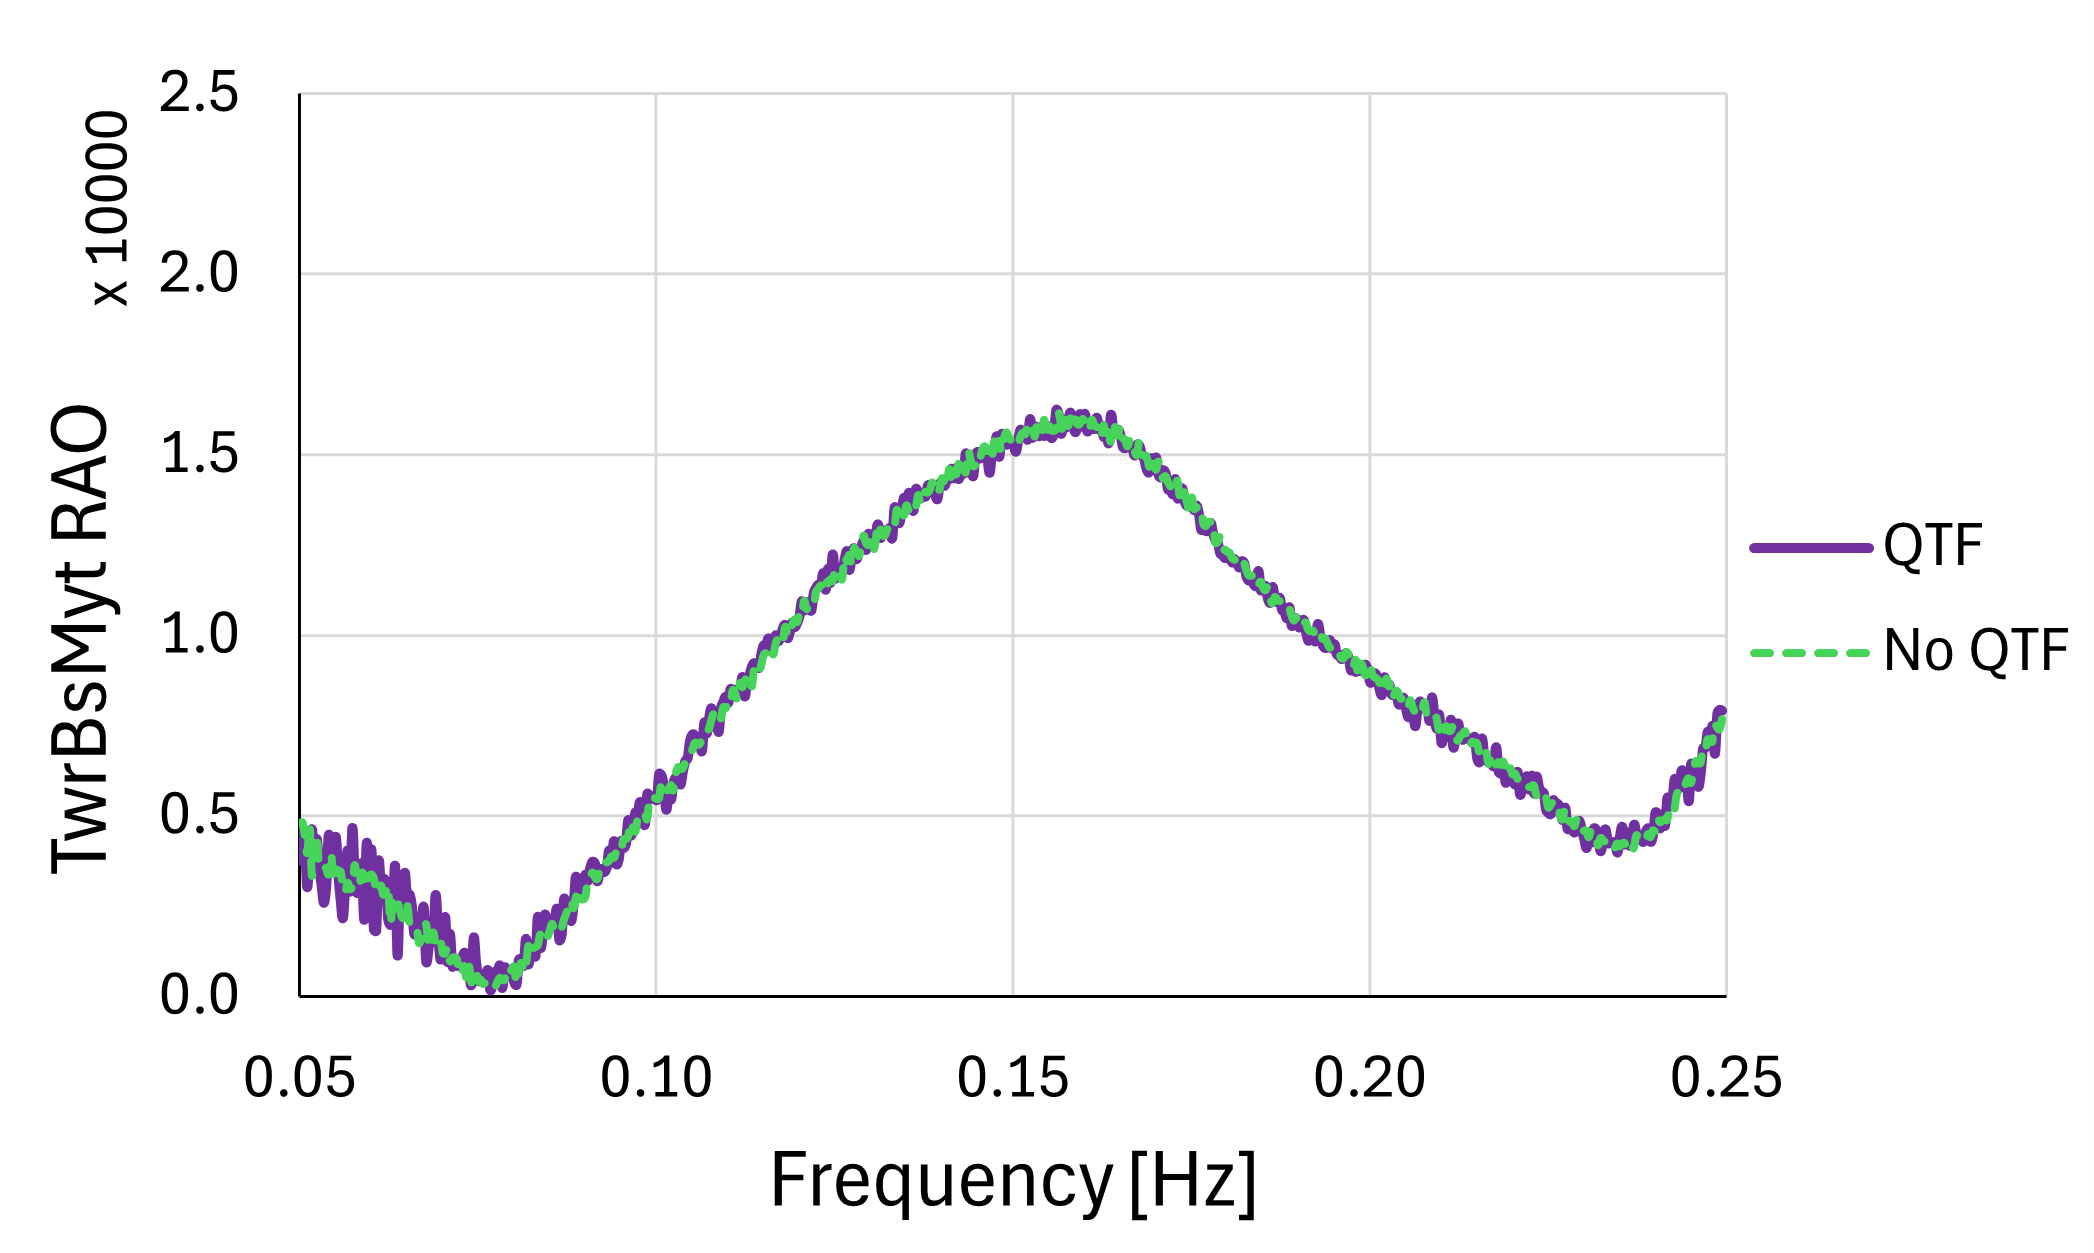
\includegraphics[width=1\textwidth]{2.6_twr_mine.png}
        \caption{\small Tower bending moment RAO} 
        \label{fig:2.6_twr_mine}
    \end{minipage}
\end{figure}

\begin{figure}[H]
    \begin{minipage}{0.48\textwidth}
        \centering
        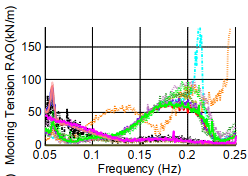
\includegraphics[width=1\textwidth]{2.6_ten.png}
        \caption{\small Mooring tension RAO \cite{Robertson2014}}
        \label{fig:2.6_fairten2}
    \end{minipage}
    \hfill
    \begin{minipage}{0.5\textwidth}
        \centering
        \vspace{0.4cm}
        \includegraphics[width=1\textwidth]{2.6_ten_mine.png}
        \caption{\small Fairlead 2 RAO}
        \label{fig:2.6_fairten2_mine}
    \end{minipage}
\end{figure}

\begin{figure}[H]
    \begin{minipage}{0.48\textwidth}
        \centering
        \includegraphics[width=1\textwidth]{2.6_surge.png}
        \caption{\small Surge RAO \cite{Robertson2014}} 
        \label{fig:2.6_surge}
    \end{minipage}
    \hfill
    \begin{minipage}{0.5\textwidth}
        \centering
        \vspace{-0.2cm}
        \includegraphics[width=1\textwidth]{2.6_surge_mine.png}
        \caption{\small Surge RAO}
        \label{fig:2.6_surge_mine}
    \end{minipage}
\end{figure}

\begin{figure}[H]
    \begin{minipage}{0.48\textwidth}
        \centering
        \includegraphics[width=1\textwidth]{2.6_heave.png}
        \caption{\small Heave RAO \cite{Robertson2014}}
        \label{fig:2.6_heave}
    \end{minipage}
    \hfill
    \begin{minipage}{0.5\textwidth}
        \centering
        \includegraphics[width=1\textwidth]{2.6_heave_mine.png}
        \caption{\small Heave RAO} 
        \label{fig:2.6_heave_mine}
    \end{minipage}
\end{figure}

\begin{figure}[H]
    \begin{minipage}{0.48\textwidth}
        \centering
        \includegraphics[width=1\textwidth]{2.6_pitch.png}
        \caption{\small Pitch RAO \cite{Robertson2014}}
        \label{fig:2.6_pitch}
    \end{minipage}
    \hfill
    \begin{minipage}{0.5\textwidth}
        \centering
        \includegraphics[width=1\textwidth]{2.6_pitch_mine.png}
        \caption{\small Pitch RAO}
        \label{fig:2.6_pitch_mine}
    \end{minipage}
\end{figure}

Both the PSD and RAO graphs show good agreement with the reference study, particularly in the non-QTF case, which exhibits fewer oscillations in the surge, heave, and pitch responses. The QTF case displays more pronounced oscillations overall, as expected, since the QTF method accounts for second-order drift effects. The PSD graphs reveal that the natural frequency of heave, approximately 0.058 Hz (Figure~\ref{fig:2.6_heave_mine}), lies within the wave excitation frequency range. This alignment significantly increases the risk of resonance, a phenomenon where the system is subjected to forces at its natural frequency, causing the amplitude of motion to grow substantially. Resonance can lead to excessive platform motions and stresses, potentially compromising the safety and integrity of the system. This effect is clearly seen in the heave RAO graph, where the peak exceeds 4 m/m, indicating a strong resonant response. In contrast, the peaks for the other degrees of freedom fall outside the dominant wave frequency range, making them less susceptible to resonance and wave-induced amplification.

\subsection{Wave and Wind Induced Tests}
\hspace*{0.5cm}The wave and wind induced tests were conducted to analyze the platform's response to various environmental conditions, including regular and irregular waves, as well as wind effects. The load cases were selected from the reference study by Robertson et al. \cite{Robertson2014} and included Group 3.X load cases. The results were processed using BEMRosetta to extract the platform's motion responses and mooring tensions.

\subsubsection{Load Case 3.1}
\hspace*{0.5cm}The load case 3.1 analyzes the platform’s response to regular airy waves with a period of 10 seconds and a significant wave height of 6 meters, and unlike load case 2.1, it includes steady and uniform wind with a speed of 8 m/s. This load case was not analyzed in the reference study, but the results were processed using BEMRosetta to extract the platform’s response, comparing the QTF and no QTF cases (Figures~\ref{fig:3.1_surge}--\ref{fig:3.1_fairten}).

\begin{figure}[H]
    \begin{minipage}{0.48\textwidth}
        \centering
        \includegraphics[width=1\textwidth]{3.1_surge.png}
        \caption{\small Surge response}
        \label{fig:3.1_surge}
    \end{minipage}
    \hfill
    \begin{minipage}{0.48\textwidth}
        \centering
        \includegraphics[width=1\textwidth]{3.1_heave.png}
        \caption{\small Heave response}
        \label{fig:3.1_heave}
    \end{minipage}
\end{figure}

\begin{figure}[H]
    \begin{minipage}{0.48\textwidth}
        \centering
        \includegraphics[width=1\textwidth]{3.1_pitch.png}
        \caption{\small Pitch response}
        \label{fig:3.1_pitch}
    \end{minipage}
    \hfill
    \begin{minipage}{0.48\textwidth}
        \centering
        \includegraphics[width=1\textwidth]{3.1_fairten.png}
        \caption{\small Fairlead 2 response}
        \label{fig:3.1_fairten}
    \end{minipage}
\end{figure}

For this load case, all degrees of freedom of the system were analyzed. Accordingly, the "B1" response was used in the result graphs, which incorporates the responses of the platform, tower, blades, and mooring system in the analysis. The results show that only the surge motion was affected by the inclusion of the second order drift effects, while the heave and pitch motions remained relatively unaffected. This is consistent with the findings from load case 2.1, where surge motion was also sensitive to second-order effects due to its weak hydrodynamic restoring forces. The fairlead 2 tension response shows a similar pattern, with some reduction in tension when neglecting second-order effects, as expected.

\subsubsection{Load Case 3.2}  
\hspace*{0.5cm}The load case 3.2 analyzes the platform’s response to irregular waves using JONSWAP spectrum with a peak wave shape parameter of 2.87, a period of 10 seconds, and a significant wave height of 6 meters, and includes turbulent wind with a speed of 11.4 m/s. For this case, the wind data was generated using both the TurbSim code included in OpenFAST files with the IECKAI model, and IEC Turbulance Simulator code made by Tecnical University of Denmark Wind Atlas Analysis and Application Program (WAsP) with the Mann model. The results were compared to those obtained from the pre-existing model (Figures~\ref{fig:3.2_ref}--\ref{fig:3.2_iec_twr}).

\begin{figure}[H]
    \centering
    \includegraphics[width=1\textwidth]{3.2_ref.png}
    \caption{\small Average responses to irregular waves and turbulent wind \cite{Robertson2014}}
    \label{fig:3.2_ref}
\end{figure}

\begin{figure}[H]
    \begin{minipage}{0.48\textwidth}
        \centering
        \includegraphics[width=1\textwidth]{3.2_turb_surge.png}
        \caption{\small Surge response from TurbSim}
        \label{fig:3.2_turb_surge}
    \end{minipage}
    \hfill
    \begin{minipage}{0.5\textwidth}
        \centering
        \includegraphics[width=0.95\textwidth]{3.2_turb_pitch.png}
        \caption{\small Pitch response from TurbSim}
        \label{fig:3.2_turb_pitch}
    \end{minipage}
\end{figure}

\begin{figure}[H]
    \begin{minipage}{0.48\textwidth}
        \centering
        \includegraphics[width=1\textwidth]{3.2_turb_twr.png}
        \caption{\small Tower bending moment response from TurbSim}
        \label{fig:3.2_turb_twr}
    \end{minipage}
    \hfill
    \begin{minipage}{0.5\textwidth}
        \centering
        \includegraphics[width=0.95\textwidth]{3.2_iec_surge.png}
        \caption{\small Surge response from IEC Turbulance Simulator}
        \label{fig:3.2_iec_surge}
    \end{minipage}
\end{figure}

\begin{figure}[H]
    \begin{minipage}{0.48\textwidth}
        \centering
        \includegraphics[width=1\textwidth]{3.2_iec_pitch.png}
        \caption{\small Pitch response from IEC Turbulance Simulator}
        \label{fig:3.2_iec_pitch}
    \end{minipage}
    \hfill
    \begin{minipage}{0.5\textwidth}
        \centering
        \includegraphics[width=0.95\textwidth]{3.2_iec_twr.png}
        \caption{\small Tower bending moment response from IEC Turbulance Simulator}
        \label{fig:3.2_iec_twr}
    \end{minipage}
\end{figure}

The results show that the platform's response to irregular waves and turbulent wind is consistent with the reference study in terms of the mean values. Both wind models yielded comparable average responses for surge, pitch, and tower bending moment. While the TurbSim model resulted in slightly greater oscillations in surge and pitch, these differences were minor and did not affect the overall trends. The tower bending moment responses were also consistent across both wind models. Overall, the results suggest that the choice between the two wind models has a limited impact on the platform’s response under the this condition. 
Additionally, the effects of the second order drift effects were limited for the pitch and tower bending moment responses, while the surge motion showed sensitivity to these effects, similar to the previous load cases. 

\section{Recreated Platform Model Analysis}

\hspace*{0.5cm}The OC4 semisubmersible platform was independently modeled in Rhino 8 (\autoref{fig:rhino}), and its hydrodynamic properties were calculated using HAMS to generate the necessary WAMIT files. The hydrostatic matrices for both the original and recreated models are presented in Figures~\ref{fig:hyd_st_org} and \ref{fig:hyd_st_re}. Notably, the recreated model’s matrix includes some coupling terms introduced by the meshing process in HAMS, which leads to small differences in the simulation results. These discrepancies are addressed in the relevant discussion sections. To evaluate the responses from the recreated model, the same set of load cases was simulated in OpenFAST for both models. In the comparison plots, results from the pre-existing model are labeled "Ex" and those from the recreated model are labeled "Re." Because the HAMS-generated WAMIT files do not provide the data required for QTF-based second-order drift analysis, the comparison uses only first-order results from the pre-existing model to ensure consistency between the simulations.

\begin{figure}[H]
    \centering
    \includegraphics[width=0.85\textwidth]{rhino.png}
    \caption{\small Recreated OC4 semisubmersible platform in Rhino}
    \label{fig:rhino}
\end{figure}

\begin{figure}[H]
    \centering
    \includegraphics[width=0.95\textwidth]{hyd_st_org.png}
    \caption{\small Hydrostatic matrix of the pre-existing model}
    \label{fig:hyd_st_org}
\end{figure}

\begin{figure}[H]
    \centering
    \includegraphics[width=0.95\textwidth]{hyd_st_re.png}
    \caption{\small Hydrostatic matrix of the recreated model}
    \label{fig:hyd_st_re}
\end{figure}

\subsection{Free Decay Tests}
\hspace*{0.5cm}The free decay tests were conducted on the recreated model, and the results were compared to those obtained from the pre-existing model. The natural frequencies were extracted from the time-domain data using the Fast Fourier Transform (FFT) method on BEMRosetta. (Figures~\ref{fig:1.3a_surge_mine_recreated}--\ref{fig:nat_freq_yaw_recreated}). 

\begin{figure}[H]
    \begin{minipage}{0.47\textwidth}
        \centering
        \includegraphics[width=1\textwidth]{1.3_surge_mine.png}
        \caption{\small Surge free decay platform motion response for load case 1.3a}
        \label{fig:1.3a_surge_mine_recreated}
    \end{minipage}
    \hfill
    \begin{minipage}{0.49\textwidth}
        \centering
        \includegraphics[width=0.95\textwidth]{1.3a_heave_mine_1.png}
        \caption{\small Heave free decay platform motion response for load case 1.3a}
        \label{fig:1.3a_heave_mine_recreated}
    \end{minipage}
\end{figure}

\begin{figure}[H]
    \begin{minipage}{0.47\textwidth}
        \centering
        \includegraphics[width=1\textwidth]{1.3a_pitch_mine_1.png}
        \caption{\small Pitch free decay platform motion response for load case 1.3a}
        \label{fig:1.3a_pitch_mine_recreated}
    \end{minipage}
    \hfill
    \begin{minipage}{0.49\textwidth}
        \centering
        \includegraphics[width=0.95\textwidth]{1.3b_surge_mine_1.png}
        \caption{\small Surge free decay platform motion response for load case 1.3b}
        \label{fig:1.3b_surge_mine_recreated}
    \end{minipage}
\end{figure}

\begin{figure}[H]
    \begin{minipage}{0.47\textwidth}
        \centering
        \includegraphics[width=1\textwidth]{1.3b_heave_mine_1.png}
        \caption{\small Heave free decay platform motion response for load case 1.3b}
        \label{fig:1.3b_heave_mine_recreated}
    \end{minipage}
    \hfill
    \begin{minipage}{0.49\textwidth}
        \centering
        \includegraphics[width=0.95\textwidth]{1.3b_pitch_mine_1.png}
        \caption{\small Pitch free decay platform motion response for load case 1.3b}
        \label{fig:1.3b_pitch_mine_recreated}
    \end{minipage}
\end{figure}

The graphs plotted for the surge motion in both load cases shows a very close resemblance to the pre-existing model, whereas the pitch and especially heave motion response shows differences in the amplitude of the oscillations. This is due to the differences in the modeling approaches and the volume calculated for the submerged part of the platform from the recreated model. The recreated model was created to closely match the dimensions and properties of the pre-existing model, but slight variations in the geometry may have led to these differences in response. The original model had a volume of 13,917 m³, while the recreated model had a volume of 13,603 m³. The difference in volume causes the bouyancy force to be different, which directly affects the heave motion response. The recreated model's heave motion response shows a higher amplitude than the pre-existing model, since the volume of the body is smaller. On the heave plot for the load case 1.3a, the green colored line represents the recreated model with the volume kept same as the original model (\autoref{fig:1.3a_heave_mine_recreated}). For this case, the recreated model's heave motion response is very close to the pre-existing model, confirming that the volume of the submerged part of the platform is a significant factor in determining the heave motion response. The recreated model's pitch motion response is also affected by the volume difference, but to a lesser extent than the heave motion response, which is presumably due to coupling effects.

%%nat frequencies recreated model
\begin{figure}[H]
    \begin{minipage}{0.47\textwidth}
        \centering
        \includegraphics[width=1\textwidth]{nat_freq_sway_1.png}
        \caption{\small Sway natural frequency}
        \label{fig:nat_freq_sway_recreated}
    \end{minipage}
    \hfill
    \begin{minipage}{0.48\textwidth}
        \centering
        \includegraphics[width=1\textwidth]{nat_freq_surge_1.png}
        \caption{\small Surge natural frequency}
        \label{fig:nat_freq_surge_recreated}
    \end{minipage}
\end{figure}

\begin{figure}[H]
    \begin{minipage}{0.47\textwidth}
        \centering
        \includegraphics[width=1\textwidth]{nat_freq_heave_1.png}
        \caption{\small Heave natural frequency}
        \label{fig:nat_freq_heave_recreated}
    \end{minipage}
    \hfill
    \begin{minipage}{0.48\textwidth}
        \centering
        \includegraphics[width=1\textwidth]{nat_freq_roll_1.png}
        \caption{\small Roll natural frequency}
        \label{fig:nat_freq_roll_recreated}
    \end{minipage}
\end{figure}

\begin{figure}[H]
    \begin{minipage}{0.47\textwidth}
        \centering
        \includegraphics[width=1\textwidth]{nat_freq_pitch_1.png}
        \caption{\small Pitch natural frequency}
        \label{fig:nat_freq_pitch_recreated}
    \end{minipage}
    \hfill
    \begin{minipage}{0.48\textwidth}
        \centering
        \includegraphics[width=1\textwidth]{nat_freq_yaw_1.png}
        \caption{\small Yaw natural frequency}
        \label{fig:nat_freq_yaw_recreated}
    \end{minipage}
\end{figure}


The natural frequencies extracted from the time-domain data were consistent with those obtained from the pre-existing model, confirming the accuracy of the recreated model. As discussed previously, the heave motion shows some difference in natural frequency, which is due to the difference in the volume of the submerged part of the platform (\autoref{fig:nat_freq_heave_recreated}). The recreated model's heave natural frequency is lower than the pre-existing model's, which is consistent with the heave motion response. Additionally, the yaw motion also presents a slight difference, which is likely a result of the different hydrostatic matrices caused by the modelling process (\autoref{fig:nat_freq_yaw_recreated}). The other degrees of freedom show very close results to the pre-existing model.

\subsection{Wave and Current Induced Tests}
\hspace*{0.5cm}In this section, the platform's response to wave and current loads was analyzed. The load cases were selected to represent both operational and extreme conditions, with varying wave and current parameters. The results were processed using BEMRosetta to extract the platform's response, comparing the recreated model to the pre-existing model.

\subsubsection{Load Case 2.1}
\hspace*{0.5cm}The load case 2.1 was used to analyze the platform’s response to regular waves, focusing on heave, pitch, surge motions, and the tension force at fairlead 2. The analysis was conducted using the pre-existing model and the recreated model and compared (Figures~\ref{fig:2.1_surge_mine_recreated}--\ref{fig:2.1_fairten2_mine_recreated}).

\begin{figure}[H]
    \begin{minipage}{0.48\textwidth}
        \centering
        \includegraphics[width=1\textwidth]{2.1_surge_mine_1.png}
        \caption{\small Surge response}
        \label{fig:2.1_surge_mine_recreated}
    \end{minipage}
    \hfill
    \begin{minipage}{0.5\textwidth}
        \centering
        \includegraphics[width=0.95\textwidth]{2.1_heave_mine_1.png}
        \caption{\small Heave response}
        \label{fig:2.1_heave_mine_recreated}
    \end{minipage}
\end{figure}

\begin{figure}[H]
    \begin{minipage}{0.48\textwidth}
        \centering
        \includegraphics[width=1\textwidth]{2.1_pitch_mine_1.png}
        \caption{\small Pitch response}
        \label{fig:2.1_pitch_mine_recreated}
    \end{minipage}
    \hfill
    \begin{minipage}{0.5\textwidth}
        \centering
        \includegraphics[width=0.95\textwidth]{2.1_fairten2_mine_1.png}
        \caption{\small Fairlead 2 response}
        \label{fig:2.1_fairten2_mine_recreated}
    \end{minipage}
\end{figure}

The results show that the surge and pitch motions are very close to the pre-existing model, while the heave motion shows a difference in the amplitude of the oscillations. This is consistent with the free decay tests, where the heave motion response was affected by the volume and slight position difference between the two models, which causes the hydrostatic restoring matrix to have coupling forces between degrees of freedom. The fairlead 2 tension response also shows a difference in amplitude, which is due to the same reason as the heave response.

\subsubsection{Load Case 2.2}
\hspace*{0.5cm}The load case 2.2 analyzes the platform's response to irregular waves, examining surge motion, pitch motion, and tower bending moment. The results were compared to those obtained from the pre-existing model (Figures~\ref{fig:2.2_surge_mine}--\ref{fig:2.2_twr_mine}). 

\begin{figure}[H]
    \centering
    \includegraphics[width=0.7\textwidth]{2.2_surge_mine.png}
    \caption{\small Surge response to irregular waves}
    \label{fig:2.2_surge_mine}
\end{figure}

\begin{figure}[H]
    \centering
    \includegraphics[width=0.7\textwidth]{2.2_pitch_mine.png}
    \caption{\small Pitch response to irregular waves}
    \label{fig:2.2_pitch_mine}
\end{figure}

\begin{figure}[H]
    \centering
    \includegraphics[width=0.7\textwidth]{2.2_twr_mine.png}
    \caption{\small Tower bending response to irregular waves (fore/aft direction)}
    \label{fig:2.2_twr_mine}
\end{figure}

Comparing the results of the recreated model to the pre-existing model, it can be observed that the mean values for both models align closely, with very similar patterns. The mean surge motion shows the largest difference with 18\% higher amplitude for the recreated model, while the pitch motion shows a 7\% lower amplitude and the tower bending moment shows a 1.4\% lower amplitude. These differences are due to the same reasons discussed previously, including the volume difference and the coupling forces in the hydrostatic matrix.

\subsubsection{Load Case 2.4 \& 2.5}

\hspace*{0.5cm}The load cases 2.4 and 2.5 were not analyzed in detail in the reference study. However, the results of these load cases were processed using BEMRosetta to extract the platform's response, comparing the recreated model to the pre-existing model (Figures~\ref{fig:2.4_surge_mine_recreated}--\ref{fig:2.5_pitch_mine_recreated}).

\begin{figure}[H]
    \begin{minipage}{0.48\textwidth}
        \centering
        \includegraphics[width=1\textwidth]{2.4_surge_mine.png}
        \caption{\small Surge response for load case 2.4}
        \label{fig:2.4_surge_mine_recreated}
    \end{minipage}
    \hfill
    \begin{minipage}{0.5\textwidth}
        \centering
        \includegraphics[width=0.95\textwidth]{2.4_heave_mine.png}
        \caption{\small Heave response for load case 2.4}
        \label{fig:2.4_heave_mine_recreated}
    \end{minipage}
\end{figure}

\begin{figure}[H]
    \begin{minipage}{0.48\textwidth}
        \centering
        \includegraphics[width=1\textwidth]{2.4_pitch_mine.png}
        \caption{\small Pitch response for load case 2.4}
        \label{fig:2.4_pitch_mine_recreated}
    \end{minipage}
    \hfill
    \begin{minipage}{0.5\textwidth}
        \centering
        \includegraphics[width=0.95\textwidth]{2.5_surge_mine.png}
        \caption{\small Surge response for load case 2.5}
        \label{fig:2.5_surge_mine_recreated}
    \end{minipage}
\end{figure}

\begin{figure}[H]
    \begin{minipage}{0.48\textwidth}
        \centering
        \includegraphics[width=1\textwidth]{2.5_heave_mine.png}
        \caption{\small Heave response for load case 2.5}
        \label{fig:2.5_heave_mine_recreated}
    \end{minipage}
    \hfill
    \begin{minipage}{0.5\textwidth}
        \centering
        \includegraphics[width=0.95\textwidth]{2.5_pitch_mine.png}
        \caption{\small Pitch response for load case 2.5}
        \label{fig:2.5_pitch_mine_recreated}
    \end{minipage}
\end{figure}

For load cases 2.4 and 2.5, which represents operational conditions with regular waves and a surface current, and extreme conditions respectively, both models exhibit similar dynamic behavior in surge, heave, and pitch. The recreated model shows a higher amplitude in heave motion, consistent with previous findings, due to its lower buoyancy. The pitch and surge responses remain closely aligned, indicating that the overall platform dynamics are well captured despite minor geometric differences. The results confirm that the recreated model is capable of replicating the general response characteristics of the pre-existing OC4 platform under both conditions.

\subsubsection{Load Case 2.6}

\hspace*{0.5cm}The load case 2.6 analyzes the platform's response to banded white noise to obtain Response Amplitudes Operators (RAOs) for the platform. The RAOs were calculated through dividing the each response PSD to the wave elevation PSD in the banded white-noise spectrum between 0.05 and 0.25 Hz and compared to the results from the pre-existing model with non-QTF case (purple plot) and recreated model (green plot) (Figures~\ref{fig:w_t_t_p_mine_recreated}--\ref{fig:2.6_pitch_mine_recreated}).

\begin{figure}[H]
    \centering
    \includegraphics[width=1\textwidth]{wave_twr_ten_psd_mine.png}
    \caption{\small Wave elevation, tower bending, and mooring tension PSD (recreated model vs. pre-existing model)}
    \label{fig:w_t_t_p_mine_recreated}
\end{figure}

\begin{figure}[H]
    \centering
    \includegraphics[width=1\textwidth]{sur_hea_pit_psd_mine.png}
    \caption{\small Sugre, heave, and pitch PSD (recreated model vs. pre-existing model)}
    \label{fig:s_h_p_p_mine_recreated}
\end{figure}

\begin{figure}[H]
    \begin{minipage}{0.48\textwidth}
        \centering
        \includegraphics[width=1\textwidth]{2.6_wave_mine_1.png}
        \caption{\small Wave elevation PSD (recreated model vs. pre-existing model)} 
        \label{fig:2.6_wave_mine_recreated}
    \end{minipage}
    \hfill
    \begin{minipage}{0.49\textwidth}
        \centering
        \vspace{-0.3cm}
        \includegraphics[width=1\textwidth]{2.6_twr_mine_1.png}
        \caption{\small Tower bending moment RAO (recreated model vs. pre-existing model)}
        \label{fig:2.6_twr_mine_recreated}
    \end{minipage}
\end{figure}

\begin{figure}[H]
    \begin{minipage}{0.48\textwidth}
        \centering
        \includegraphics[width=0.95\textwidth]{2.6_ten_mine_1.png}
        \caption{\small Mooring tension RAO (recreated model vs. pre-existing model)}
        \label{fig:2.6_ten_mine_recreated}
    \end{minipage}
    \hfill
    \begin{minipage}{0.48\textwidth}
        \centering
        \includegraphics[width=1\textwidth]{2.6_surge_mine_1.png}
        \caption{\small Surge RAO (recreated model vs. pre-existing model)} 
        \label{fig:2.6_surge_mine_recreated}
    \end{minipage}
\end{figure}

\begin{figure}[H]
    \begin{minipage}{0.48\textwidth}
        \centering
        \includegraphics[width=1\textwidth]{2.6_heave_mine_1.png}
        \caption{\small Heave RAO (recreated model vs. pre-existing model)}
        \label{fig:2.6_heave_mine_recreated}
    \end{minipage}
    \hfill
    \begin{minipage}{0.48\textwidth}
        \centering
        \includegraphics[width=1\textwidth]{2.6_pitch_mine_1.png}
        \caption{\small Pitch RAO (recreated model vs. pre-existing model)}
        \label{fig:2.6_pitch_mine_recreated}
    \end{minipage}
\end{figure}

From the results of the PSD and RAO graphs, it can be seen that the recreated model shows a good agreement with the pre-existing model, particularly in the non-QTF case with less oscillations. As expected, the heave RAO amplitude is higher than the pre-existing model, which is consistent with the heave motion response. The tower bending moment RAO also shows a higher amplitude, which is caused by higher tower bending moments in the recreated model. The surge and pitch RAOs show a very close resemblance to the pre-existing model, indicating that the overall platform dynamics are well captured despite geometric differences. The results confirm that the recreated model is capable of replicating the general response characteristics of the pre-existing OC4 platform under banded white noise conditions.

\subsection{Wave and Wind Induced Tests}
\hspace*{0.5cm}In this section, the recreated model's response to combined wave and wind loads was analyzed. The load cases were selected to represent both operational and extreme conditions, with varying wave and wind parameters. The results were processed using BEMRosetta to extract the platform's response, comparing the recreated model to the pre-existing model.

\subsubsection{Load Case 3.1}
\hspace*{0.5cm}The load case 3.1 analyzes the platform's response to regular airy waves with a period of 10 seconds and a significant wave height of 6 meters, and includes steady and uniform wind with a speed of 8 m/s. This load case was not analyzed in the reference study, but the results were processed using BEMRosetta to extract the platform's response, comparing the recreated model to the pre-existing model (Figures~\ref{fig:3.1_surge_mine_recreated}--\ref{fig:3.1_fairten_mine_recreated}).

\begin{figure}[H]
    \begin{minipage}{0.48\textwidth}
        \centering
        \includegraphics[width=1\textwidth]{3.1_surge_mine.png}
        \caption{\small Surge response (recreated model vs. pre-existing model)}
        \label{fig:3.1_surge_mine_recreated}
    \end{minipage}
    \hfill
    \begin{minipage}{0.5\textwidth}
        \centering
        \includegraphics[width=0.95\textwidth]{3.1_heave_mine.png}
        \caption{\small Heave response (recreated model vs. pre-existing model)}
        \label{fig:3.1_heave_mine_recreated}
    \end{minipage}
\end{figure}

\begin{figure}[H]
    \begin{minipage}{0.48\textwidth}
        \centering
        \includegraphics[width=1\textwidth]{3.1_pitch_mine.png}
        \caption{\small Pitch response (recreated model vs. pre-existing model)}
        \label{fig:3.1_pitch_mine_recreated}
    \end{minipage}
    \hfill
    \begin{minipage}{0.5\textwidth}
        \centering
        \includegraphics[width=0.95\textwidth]{3.1_fairten_mine.png}
        \caption{\small Fairlead 2 response (recreated model vs. pre-existing model)}
        \label{fig:3.1_fairten_mine_recreated}
    \end{minipage}
\end{figure}

The results show that the surge and pitch motions are very close to the pre-existing model, while the heave motion shows a difference in the amplitude of the oscillations. This is consistent with the free decay tests, where the heave motion response was affected by the volume and slight position difference between the two models, which causes the hydrostatic restoring matrix to have coupling forces between degrees of freedom. The fairlead 2 tension response also shows a difference in amplitude, which is due to the same reason as the heave response. Overall, the recreated model's response to regular waves and steady wind is consistent with the pre-existing model, confirming that it can accurately capture the platform's dynamic behavior under these conditions.

\subsubsection{Load Case 3.2}
\hspace*{0.5cm}The load case 3.2 analyzes the platform's response to irregular waves using JONSWAP spectrum. The results were compared to those obtained from the pre-existing model (Figures~\ref{fig:3.2_turb_surge_mine_recreated}--\ref{fig:3.2_iec_twr_mine_recreated}).

\begin{figure}[H]
    \begin{minipage}{0.48\textwidth}
        \centering
        \includegraphics[width=1\textwidth]{3.2_turb_surge_mine.png}
        \caption{\small Surge response from TurbSim (recreated model vs. pre-existing mode)}
        \label{fig:3.2_turb_surge_mine_recreated}
    \end{minipage}
    \hfill
    \begin{minipage}{0.5\textwidth}
        \centering
        \includegraphics[width=0.95\textwidth]{3.2_turb_pitch_mine.png}
        \caption{\small Pitch response from TurbSim (recreated model vs. pre-existing mode)}
        \label{fig:3.2_turb_pitch_mine_recreated}
    \end{minipage}
\end{figure}

\begin{figure}[H]
    \begin{minipage}{0.48\textwidth}
        \centering
        \includegraphics[width=1\textwidth]{3.2_turb_twr_mine.png}
        \caption{\small Tower bending moment response from TurbSim (recreated model vs. pre-existing model)}
        \label{fig:3.2_turb_twr_mine_recreated}
    \end{minipage}
    \hfill
    \begin{minipage}{0.5\textwidth}
        \centering
        \includegraphics[width=0.95\textwidth]{3.2_iec_surge_mine.png}
        \caption{\small Surge response from IEC Turbulance Simulator (recreated model vs. pre-existing model)}
        \label{fig:3.2_iec_surge_mine_recreated}
    \end{minipage}
\end{figure}

\begin{figure}[H]
    \begin{minipage}{0.48\textwidth}
        \centering
        \includegraphics[width=1\textwidth]{3.2_iec_pitch_mine.png}
        \caption{\small Pitch response from IEC Turbulance Simulator (recreated model vs. pre-existing model)}
        \label{fig:3.2_iec_pitch_mine_recreated}
    \end{minipage}
    \hfill
    \begin{minipage}{0.5\textwidth}
        \centering
        \includegraphics[width=0.95\textwidth]{3.2_iec_twr_mine.png}
        \caption{\small Tower bending moment response from IEC Turbulance Simulator (recreated model vs. pre-existing model)}
        \label{fig:3.2_iec_twr_mine_recreated}
    \end{minipage}
\end{figure}

The results show that the platform's response to irregular waves and turbulent wind is in the recreated model is very similar to that of the pre-existing model, with minor differences in the mean values. For both wind models used, the results were almost identical to those from the existing model. The recreated model showed a slightly higher mean value for surge motion ($\sim$0.8\%), and slightly lower mean values for pitch and tower bending moment ($\sim$2.3\%). These small differences are in line with what was observed in previous load cases. Overall, the recreated model is able to accurately represent the platform's dynamic behavior under irregular wave and turbulent wind conditions. This agreement confirms the validity of the recreation process and the accuracy of the hydrodynamic properties calculated using HAMS.

\section{Conclusion}

\hspace*{0.5cm}This report examined the numerical modeling and dynamic analysis of the OC4 semisubmersible platform using both a pre-existing OpenFAST model, and a recreated model developed in Rhino 8, with hydrodynamic analysis performed in HAMS. The primary objective was to validate the platform's behavior under various environmental loads, including free decay tests, regular and irregular waves, and combined wave and wind loads, while also demonstrating the applicability of modern tools such as HAMS and OpenFAST in offshore platform analysis

The pre-existing model's results aligned closely with the results of the participants who used similar tools and methods in the reference study \cite{Robertson2014} to the ones used in this study. The free decay tests confirmed the platform's natural periods and damping characteristics, while wind and wave induced load cases demonstrated the platform's responses to various environmental loads. Notably, the significant impact of second-order drift effects on the surge motion and the risk of resonance in the heave motion were found as a result of the analysis. These findings have direct implications for real-world applications, as excessive motions or resonance could lead to structural damage or failure.

The recreated model successfully reproduced the general behavior of the pre-existing model, with minor deviations primarily due to differences in submerged volume and coupling effects in the hydrostatic matrix. These were addressed in the analysis, confirming the reliability of the recreated model for simulating offshore wind platforms.

While the 2014 reference study provided a solid foundation, this report has expanded on that work by implementing a modern modeling environment and validating its performance. The findings demonstrate the value of updated simulation tools in offshore wind research, supporting their use in continued efforts to improve accuracy, safety, and long-term reliability of floating renewable energy systems.


\newpage
\begin{thebibliography}{99}
\addcontentsline{toc}{section}{References}

\bibitem{Robertson2014} Robertson, A. N., Jonkman, J., and Musial, W. (2014). \textit{OC4-DeepCwind Semi-Submersible Baseline Control System Design}. National Renewable Energy Laboratory (NREL), Golden, CO.
\bibitem{metacenter} Jonkman, J. M. (2007). \textit{Dynamics modeling and loads analysis of an offshore floating wind turbine} (Technical Report NREL/TP-500-41958). National Renewable Energy Laboratory. https://www.nrel.gov/docs/fy07osti/41958.pdf
\bibitem{RAO} Faltinsen, O. M. (1990). \textit{Sea loads on ships and offshore structures}. Cambridge University Press.


\end{thebibliography}

\end{document}